
% Para 'Draft Version'/'Versao Preliminar' com data no rodape, adicionar 'dv':
%   \documentclass[dsc, dv]{ita} 
% Para trabalhos em Inglês, adicionar 'eng':
%   \documentclass[dsc, eng]{ita}
%		\documentclass[dsc, eng, dv]{ita}

\documentclass[tg, eng]{ita}    % ITA.cls based on standard book.cls 
  % \documentclass[tg]{ita}			= Trabalho de Graduacao
%   								msc     		= Dissertacao de Mestrado
%   								dsc      		= Tese de Doutorado


% Quando alterar a classe, por exemplo de [msc] para [msc, eng]) rode mais uma vez o botão BUILD OUTPUT caso haja erro

\usepackage{ae}
\usepackage{epsfig}
\usepackage{amsthm}
\usepackage{amsmath}
\usepackage{amssymb}
\usepackage{multirow}
\usepackage{float}
\usepackage{booktabs}
\usepackage[section]{placeins}
\usepackage{pdfpages}

\usepackage{longtable}
\usepackage{listings}
\usepackage{tikz}
\usepackage{graphicx}
\usepackage{subcaption}
\usepackage[inkscapeformat=png]{svg}
\usetikzlibrary{shapes.geometric, arrows}
\lstset{basicstyle=\ttfamily,
  showstringspaces=false,
  commentstyle=\color{red},
  keywordstyle=\color{blue}
}
\usepackage[T1]{fontenc}
\usepackage{minted}

\usepackage{fancyvrb}
\usepackage{algorithm}
\usepackage{algpseudocode}
\usepackage{forest}
\usepackage{svg}

\tikzset{
    halfandhalf/.style n args={3}{
        path picture={
            \begin{scope}
                \clip (path picture bounding box);
                % Left half
                \fill[#1] (path picture bounding box.south west) rectangle
                          (path picture bounding box.north);
                % Right half
                \fill[#2] (path picture bounding box.south) rectangle
                          (path picture bounding box.north east);
            \end{scope}
            \node[align=center] at (path picture bounding box.center) {#3};
        }
    }
}


%++++++++++++++++++++++++++++++++++++++++++++++++++++++++++++++++++++++++++++++
% Espaçamento padrão de todo o documento
%++++++++++++++++++++++++++++++++++++++++++++++++++++++++++++++++++++++++++++++
\onehalfspacing

%singlespacing Para um espaçamento simples
%onehalfspacing Para um espaçamento de 1,5
%doublespacing Para um espaçamento duplo

%++++++++++++++++++++++++++++++++++++++++++++++++++++++++++++++++++++++++++++++
% Identificacoes (se o trabalho for em inglês, insira os dados em inglês)
% Para entradas abreviadas de Professora (Profa.) em português escreva: Prof$^\textnormal{a}$.
%++++++++++++++++++++++++++++++++++++++++++++++++++++++++++++++++++++++++++++++
\course{Computer Engineering} % Programa de PG ou Curso de Graduação
% \area{Sistemas Aeroespaciais e Mecatrônica} % Área de concentração na PG (Não utilizado no caso de TG)

% Autor do trabalho: Nome Sobrenome
\authorgender{masc} %sexo: masc ou fem
\author{Rafael}{Studart Mattos Di Piero}
\itaauthoraddress{Rua do H8A, Ap. 125}{12.228-460}{São José dos Campos--SP}


% Titulo da Tese/Dissertação
\title{Multi-Agent Graph Exploration Without Communication}

% Orientador
\advisorgender{masc}                    % masc ou fem
\advisor{Prof.~Dr.}{Luiz Gustavo Bizarro Mirisola}{ITA}

% Coorientador 
\coadvisorgender{masc} % masc ou fem
\coadvisor{Prof.~Dr.}{Vitor Venceslau Curtis}{ITA}

% Pró-reitor da Pós-graduação
%\bossgender{masc}  % masc ou fem
%\boss{Prof.~Dr.}{Sicrano}

%Coordenador do curso no caso de TG
\bosscoursegender{masc}	% masc ou fem
\bosscourse{Prof.~Dr.}{Marcos Ricardo Omena de Albuquerque Máximo}

% Palavras-Chaves informadas pela Biblioteca -> utilizada na CIP
\kwcip{Graph}
\kwcip{Search}
\kwcip{Multi-agent}
\kwcip{Mixed Radix}
% membros da banca examinadora

\examiner{Prof. Dr.}{Luiz Gustavo Bizarro Mirisola}{Presidente}{ITA}
\examiner{Prof. Dr.}{Vitor Venceslau Curtis}{}{ITA}
% \examiner{Prof. Dr.}{Karla Donato Fook}{}{ITA}

% Data da defesa (mês em maiúsculo, se trabalho em inglês, e minúsculo se trabalho em português) 
\date{20}{Nov}{2024}

% Número CDU - (somente para TG)
\cdu{CDU}

% Glossario
\makeglossary
\frontmatter

\begin{document}
% Folha de Rosto e Capa para o caso do TG
\maketitle

% Dedicatoria:
\begin{itadedication}
  To my family, for their love and constant support. 
  To my friends, for standing by me through all moments. 
\end{itadedication}

% Agradecimentos
\begin{itathanks}
I want to express my gratitude to:

My family, for their unwavering support and love throughout my studies.

My friends from H8 and Fortaleza, for their constant encouragement and companionship.

Prof. Dr. Luiz Gustavo Bizarro Mirisola for his guidance and patience as my advisor.
\end{itathanks}


% Epígrafe
\thispagestyle{empty}
\ifhyperref\pdfbookmark[0]{\nameepigraphe}{epigrafe}\fi
\begin{flushright}
\begin{spacing}{1}
\mbox{}\vfill
{\sffamily\itshape
"The journey of a thousand miles begins with one step."\\
}
--- \textsc{
Lao Tzu
}
\end{spacing}
\end{flushright}

% Resumo
\begin{abstract}
\noindent
A teoria dos grafos, um campo fundamental da matemática e da ciência da computação, oferece estruturas robustas para modelar relacionamentos e percorrer estruturas de grafos. Esta pesquisa se aprofunda na exploração de grafos, crucial para aplicações como roteamento de redes, robótica e geração procedural. Como as aplicações do mundo real frequentemente envolvem ambientes complexos com restrições de tempo, como operações de busca e resgate com drones, este estudo foca em sistemas multiagente para a exploração de grafos, onde múltiplos agentes autônomos colaboram para otimizar a distribuição de tarefas.

Este trabalho apresenta uma estrutura modular estruturada em classes extensíveis, facilitando a adição de novos algoritmos e conjuntos de dados. Ao ir além das limitações da exploração de labirintos perfeitos \cite{Naeem2021}, empregamos o NetworkX \cite{Hagberg2008}—uma biblioteca de grafos geral—que permite a análise de estruturas de grafos mais diversas. Essa flexibilidade possibilitou comparações em diversos conjuntos de dados para revelar padrões no desempenho dos algoritmos sob diferentes características dos grafos.

O objetivo deste estudo é propor um algoritmo multiagente eficiente para exploração de grafos sem comunicação, uma necessidade crucial em cenários onde a comunicação é impraticável ou impossível. Baseando-se no método de exploração de labirintos perfeitos detalhado por \citen{Arthur2023}, este estudo estende a abordagem para grafos gerais, incluindo aqueles com ciclos, e avalia o desempenho do algoritmo em quatro conjuntos de dados de complexidade variada. Ao estabelecer um benchmark para a eficiência da exploração, esta pesquisa permite uma avaliação dos custos e benefícios da incorporação da comunicação em estratégias multiagente, proporcionando uma base comparativa para o desenvolvimento futuro de algoritmos de exploração.

Além disso, esta pesquisa incorporou heurísticas e estratégias alternativas para aprimorar o algoritmo de Tarry, que tradicionalmente depende da seleção aleatória de vizinhos. As adaptações resultantes demonstraram melhorias de desempenho em conjuntos de dados específicos, ilustrando como processos de seleção direcionados podem otimizar a eficiência da exploração com base nas propriedades dos conjuntos de dados.
\end{abstract}

% Abstract
\begin{englishabstract}
\noindent
Graph theory, a pivotal field in mathematics and computer science, offers robust frameworks for modeling relationships and traversing graph structures. This research delves into graph exploration, crucial for applications like network routing, robotics, and procedural generation. As real-world applications often involve complex environments with time constraints, such as search-and-rescue operations with drones, this study focuses on multi-agent systems for graph exploration, where multiple autonomous agents collaborate to optimize task distribution.

This work presents a modular framework structured into extensible classes, facilitating the addition of new algorithms and datasets. By moving beyond the constraints of perfect maze exploration \cite{Naeem2021}, we employed NetworkX \cite{Hagberg2008}—a general graph library—which allows for analyzing more diverse graph structures. This flexibility enabled comparisons across various datasets to reveal patterns in algorithm performance under different graph characteristics.

This study's objective is to propose an efficient multi-agent algorithm for graph exploration without communication, a crucial need in scenarios where communication is impractical or impossible. Building on the method for perfect maze exploration detailed by \citen{Arthur2023}, this study extends the approach to general graphs, including those with cycles, and evaluates the algorithm's performance across three datasets of varying complexity. By establishing a benchmark for exploration efficiency, this research enables an assessment of the costs and benefits of incorporating communication in multi-agent strategies, providing a comparative baseline for future exploration algorithm development.

Additionally, this research incorporated heuristics and alternative strategies to enhance Tarry's algorithm, which traditionally relies on random neighbor selection. The resulting adaptations demonstrated performance improvements on specific datasets, illustrating how targeted selection processes can optimize exploration efficiency based on dataset properties. These insights pave the way for future research into more effective graph exploration strategies in autonomous systems.
\end{englishabstract}

% Lista de figuras
\listoffigures %opcional

% Lista de tabelas
% \listoftables %opcional

% Lista de Algoritmnos
\listofalgorithms %opcional

% Lista de abreviaturas
\listofabbreviations
\begin{longtable}{ll}
$DFT$ density functional theory \\
$HF$ hartree-fock \\
$GMSN$ group of semiconductors materials and nanotechnology\\
$CLI$ command line interface \\
$HK$ hohenberg-kohn \\
$LDA$ local density approximation \\
$GGA$ generalized gradient approximation \\
$PBE$ perdew-burke-ernzerhof \\
$VBM$ valence band maximum \\
$CBM$ conduction band minimum \\
$GUI$ graphical user interface \\
$VASP$ vienna ab initio simulation package \\
$RMSE$ root mean square error \\
$VESTA$ visualization for electronic and structural analysis \\
\end{longtable} %opcional

% Lista de simbolos
\listofsymbols
\begin{longtable}{ll}

$G$ Graph \\
$v_n$ Vertex \\
$v_nv_m$ Edge \\

\end{longtable} %opcional

% Sumario
\tableofcontents

\mainmatter
% Os capitulos comecam aqui

\chapter{Introduction}
\section{Motivation}
\label{section_intro_motivation}

Graph theory is a fundamental field of mathematics with significant relevance in
computer science due to its ability to model relationships between objects.
One of the key challenges in computer science is graph traversal and exploration, which involves systematically navigating through the nodes of a graph
with a specific purpose. This topic has practical applications across diverse fields, such as network routing, robotics, procedural generation, electronics design, and more.

When considering the complexities and time constraints imposed by real-world environments,
graph exploration must be expanded to consider multi-agent systems. In such systems, multiple
autonomous agents collaborate to explore graphs, aiming to distribute tasks to achieve optimal efficiency. However, communication strategies
on these systems are challenging, as they need to balance the trade-off between the amount of information shared among agents
versus the quality of the solution. In other words, while communication can allow
agents to speed up their exploration, it may cost time and/or energy.

Various versions of this problem have been explored in research. 
One such approach, discussed by \citen{Kivelevitch2010}, proposed a generalization of Tarry's Algorithm with significant emphasis on minimizing data transfer.
Nevertheless, this solution is limited to mazes and does not extend to general graphs.

Despite the previously mentioned research, the concept of zero-communication exploration has not been
concretely established in the literature. We believe this gap is significant, as practical situations might involve
scenarios where communication is limited or impossible due to bandwidth limitations or energy consumption, such as deep-sea exploration,
search with energy-limited agents, or high-efficiency state space search. 

This work aims to address this gap by presenting a continuation
and expansion of a method initially developed for perfect maze exploration \cite{Naeem2021} as discussed by \citen{Arthur2023}.
Building upon this groundwork, the research extends the method to accommodate diverse graph structures by removing dependencies on specific projects. 
General improvements, such as structuring the exploration into well-defined and extensible classes
and incorporating built-in testing, strive to make the development process more versatile and robust, paving the way for broader applications in multi-agent systems.


\section{Objective}
\label{section_intro_objective}

This study aims to propose a viable algorithm for graph exploration by multi-agents, specifically targeting the identification of a goal node.
A previous paper by \citen{Arthur2023} discussed an approach for perfect maze exploration, which can be modeled as a tree, a connected acyclic undirected graph.
Expanding the proposed algorithm to connected cyclic graphs could allow further discussion and contribute to research in real-world applications 
such as robotics, as well as in the theoretical analysis of parallelism and communication between agents.

\section{Definitions}
\label{section_intro_definitions}

This section aims to define key concepts in graph theory and
multi-agent exploration that are essential for understanding the context 
and methodology of our research, ensuring clarity and consistency in the subsequent discussions.

\subsection{Graph}
\label{section_definitions_graph}

Graphs are structures in mathematics and computer science used to represent
relationships between pairs of objects. According to \citen{Manber1989}, a graph
$G=(V,E)$ is defined as a set $V$ of vertices (or nodes) and a set $E$ of edges,
that connect pairs of vertices. 

\subsubsection{Common Nomenclature}

In graph theory, the basic terminology includes the following components:

\begin{itemize}
    \item Vertex (Node): The fundamental unit of a graph, representing an object or a point.
    \item Edge: A connection between a pair of vertices, representing a relationship between them.
    \item Adjacency: Two vertices $v$ and $w$ of a graph $G$ are adjacent if there is an edge $vw$ joining them, and the vertices $v$ and $w$ are then incident with such an edge. \cite{West2018}
    \item Degree: Degree of a vertex $v$ of $G$ is the number of edges incident with $v$. \cite{West2018}
    \item Path: A path in a graph $G$, as defined by \citen{West2018}, is a finite sequence of edges of the form $v_0v_1$, $v_1v_2$, ... in which any two consecutive edges are adjacent, all edges are distinct and all vertices $v_0$, $v_1$, ..., $v_m$ are distinct (except, possibly, $v_0 = v_m$).
    \item Cycle: A path where $v_0 = v_m$ and with at least one edge. \cite{West2018}
\end{itemize}

\subsubsection{Key Properties}

A few key properties of graphs that interest us are:

\begin{itemize}
    \item Connectivity: A graph is connected if and only if there is a path between each pair of vertices. \cite{West2018}
    \item Acyclicity: A graph is acyclic if it has no cycles. A tree is an acyclic connected graph.
\end{itemize}

\subsubsection{Traversal}

Graph traversal is the process of visiting all the vertices in a graph in a systematic manner. Two fundamental algorithms for graph traversal are:

\begin{itemize}
    \item Breadth-first search (BFS): Expands the frontier between discovered and undiscovered vertices uniformly across the breadth of the frontier. \cite{Manber1989}
    \item Depth-first search (DFS): Explores edges out of the most recently discovered vertex $v$ that still has unexplored edges leaving it. \cite{Manber1989}
    \item Tarry's Algorithm: Tarry's Algorithm is used traverse the entire maze, or graph, in a depth first fashion, where each edge is travelled twice, and the agent finishes the motion at the same initial vertex it started from.\cite{Kivelevitch2010} This algorithm is described in the context of a physical maze, where the agent must physically move between adjacent nodes.
    It was first described over botanical mazes built as amusements for the XIX century aristocracy.
\end{itemize}

\subsection{Agent}
\label{section_definitions_agent}

An agent in maze exploration, as defined by \citen{Kivelevitch2010}, 
is an entity able to move within the maze in any direction as long as it does not encounter obstacles.

In the context of graph exploration, this concept extends to an agent's ability to traverse
edges between vertices within the graph structure. Each agent acts independently,
making decisions based on its individual memory and the local information available at its current vertex and its adjacent edges.


\subsection{Mixed Radix}
\label{section_definitions_mixed_radix}

A mixed radix system is a positional numerical system in which the numerical base for each digit
varies. This allows for more flexible representation of numbers,
accommodating various scales within the same numerical framework.

One mathematical approach for representing mixed radix numbers can be found in \citen{Arndt2011},
which establishes a comprehensive arithmetical method for manipulating them.  However,
for the specific subset of real numbers within the interval [0, 1], a more specialized approach is utilized, as described by \citen{Arthur2023}.

In this context, the mixed radix representation $A=[a_{0},a_{1},a_{2},...,a_{n-1}]$ 
of a number $x$ with respect to a radix vector $M=[m_{0},m_{1},m_{2},...,m_{n-1}]$,
where $x \in [0,1]$, is given by:

\begin{equation}
	x = \sum_{k=0}^{n-1} a_{k} \prod_{j=0}^{k} \frac{1}{m_j}
\end{equation}
where $a_j$ are non-negative integers, $m_j$ are integers such that $m_j \geq 2$, and $0 \leq a_j \leq m_j$. \cite{Arthur2023}


For instance, if $x$ is represented by $2_{3}1_{2}1_{4}0_{3}1_{5}$, and considering that $a_{i}$ is on the left of $a_{i+1}$, $x$ might be transformed to the decimal base by the following steps:

\begin{align}
& x=2_{3}1_{2}1_{4}0_{3}1_{5}\\
& A=[2,1,1,0,1]\\
& M=[3,2,4,3,5]\\
& n=5\\
& x = \sum_{k=0}^{4} a_{k} \prod_{j=0}^{k} \frac{1}{m_j} \approx 0.8777778
\end{align}

\subsubsection{Extending Mixed Radix with Unary Digits}

In our study, we extended the mixed radix system to include unary digits,
which are used to represent steps in a sequence where no meaningful decisions are made.
These unary digits do not contribute to the numerical value and can be omitted in the conversion to standard numerical forms.

Within our framework, the mixed radix representation $A=[a_{0},a_{1},a_{2},...,a_{n-1}]$ 
of a number $x$ with respect to a radix vector $M=[m_{0},m_{1},m_{2},...,m_{n-1}]$,
where $x \in [0,1]$, is given by:

Let  $U = \{ k \ |\ m_k \neq 1 \} $ be the set of indices where the base \( m_k \) is not unary.

\begin{equation}
	x = \sum_{k \in U} u_{k} \prod_{j=0}^{k} \frac{1}{m_j}
\end{equation}
where $a_k$ are non-negative integers, $m_j$ are integers such that $m_j \geq 1$, and $0 \leq a_j \leq m_j$.

Consider the mixed radix representation $x=2_{3}X_11_{2}X_1X_11_{4}0_{3}1_{5}$, where $X_1$ represents the unary digit and each $a_{i}$ is on the left of $a_{i+1}$. We can transform
$x$ to the decimal base using the following steps:

\begin{align}
    & x=2_{3}X_11_{2}X_1X_11_{4}0_{3}1_{5}\\
    & A=[2,X,1,X,X,1,0,1]\\
    & M=[3,1,2,1,1,4,3,5]\\
    & U=[0,2,5,6,7]\\
    & x = \sum_{k \in U} a_{k} \prod_{j=0}^{k} \frac{1}{m_j} \approx 0.8777778
\end{align}


\chapter{Methodology}
This section intends to discuss specific design choices that support
our multi-agent search algorithm.
Section \ref{section_method_modeling} introduces the models and classes developed to improve our algorithm.
Section \ref{section_method_algorithm} describes the core concepts of our algorithm and provides pseudocode to guide its implementation.
Section \ref{section_method_mixed_radix} presents a mixed radix numerical representation used for the agent's path and examples to demonstrate its functionality.
Finally, \ref{section_method_alt_exploration_alg} details how we can extend our solution to allow different exploration algorithms.

\section{Modeling}
\label{section_method_modeling}

In this section, we detail the modeling approach chosen to structure our problem,
emphasizing the use of classes to achieve greater flexibility in our solution.
The main classes include \textbf{Simulation},\textbf{Graph} and \textbf{Agent}, each of which will be defined in subsequent sections.
Figure \ref{fig:class_diagram} presents a simplified class diagram that illustrates the overall structure of our model.

\begin{figure}[ht!]
    \centering
    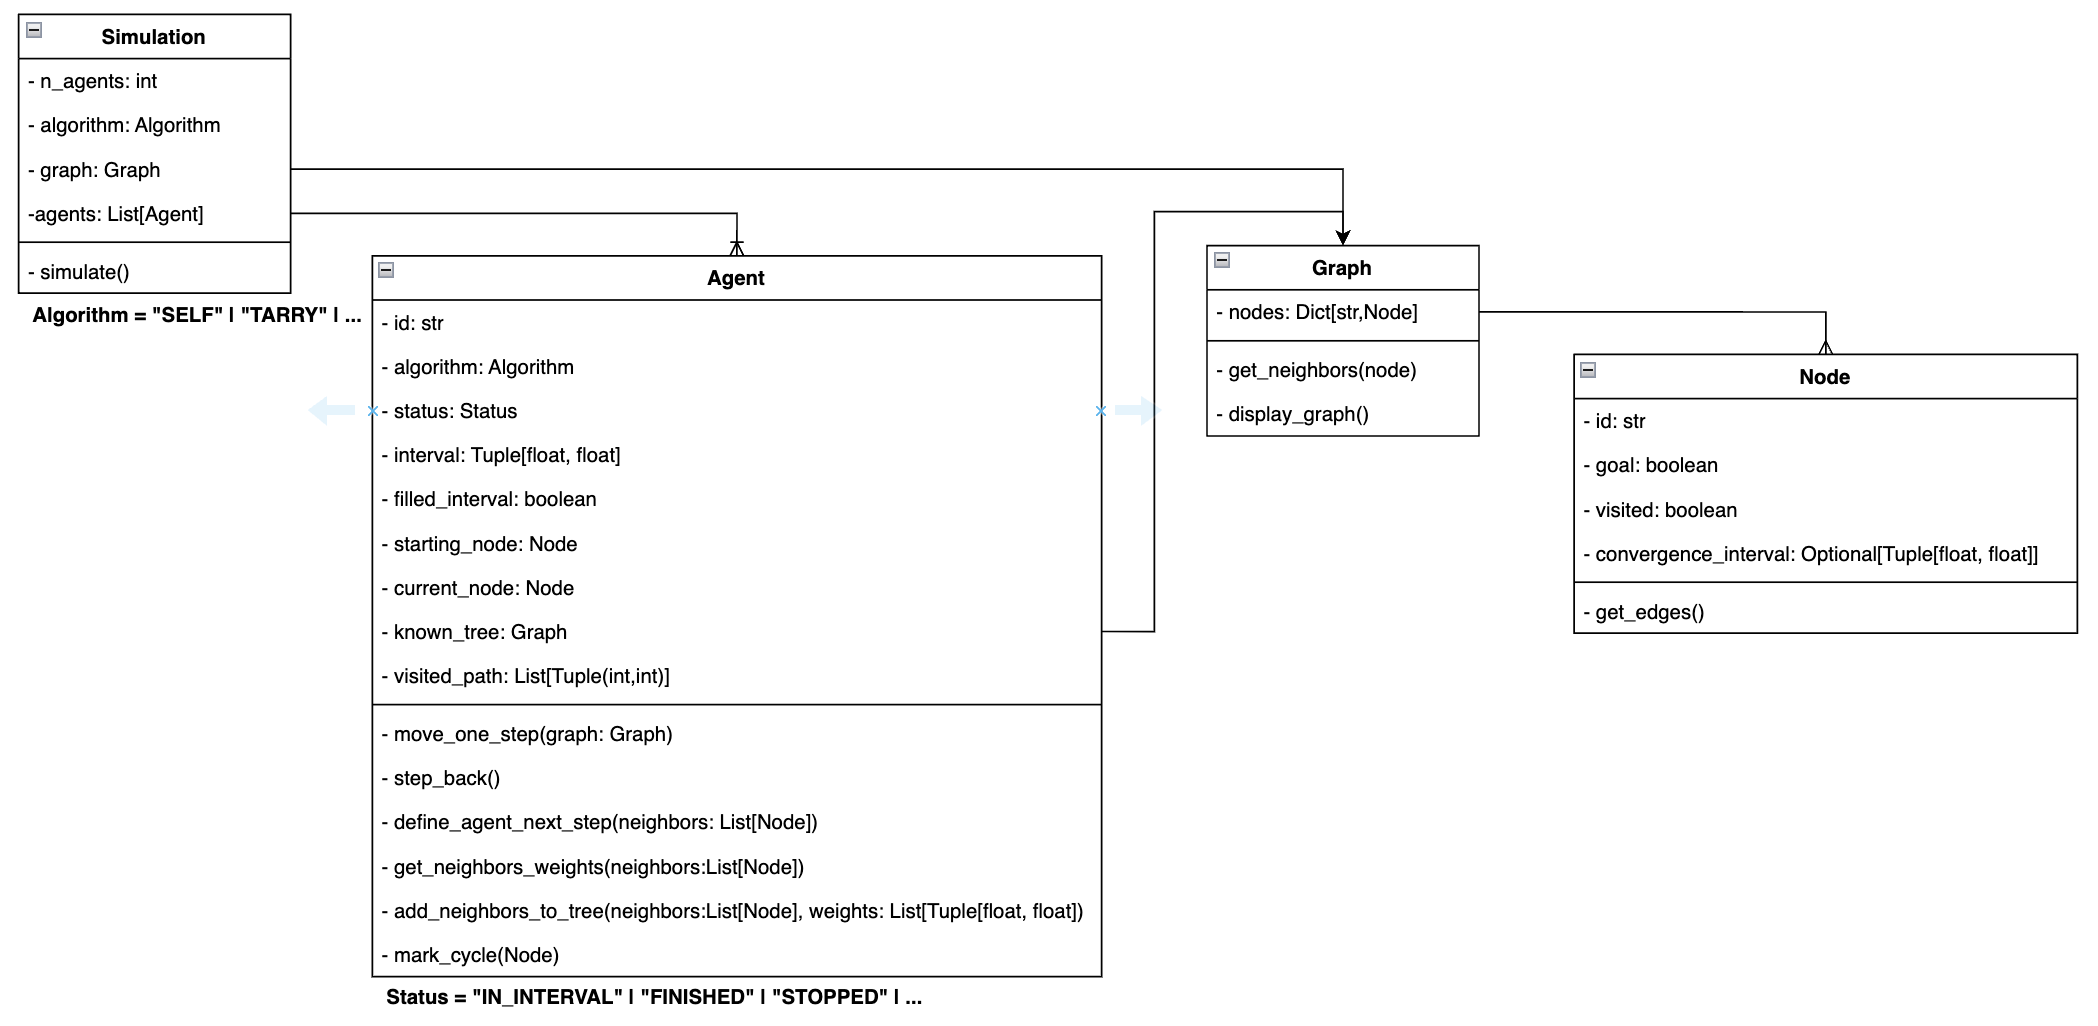
\includegraphics[width=0.9\textwidth]{Cap2/simplified_class_diagram.png}
    \caption{Simplified Class Diagram of the Multi-Agent Maze Exploration Model}
    \label{fig:class_diagram}
\end{figure}

\subsection{Simulation}
\label{section_modeling_simulation}

The \textbf{Simulation} class acts as a central controller in our multi-agent
graph exploration problem. It is primarily responsible for managing shared information, including the graph structure.
Additionally, it orchestrates the agents and the overall execution of the exploration process.

In more detail, its responsibilities include:

\begin{itemize}
    \item Shared Information: Storing and managing all information that is common between agents.
    \item Orchestration: Coordination agent activities and possible interactions during the exploration.
    \item Visualization: Providing tools for tracking the progress and visualizing the result of the exploration.
    \item Metrics: Collecting and analyzing performance metrics of the exploration.
\end{itemize}

As shown by Figure \ref{fig:class_diagram}, the core method of the \textbf{Simulation} is $simulate$ that is responsible for starting the exploration and managing each agent
in parallel, until all agents have reached the goal or have no more moves available.
The pseudocode in Algorithm \ref{alg:simulate} provides a breakdown of the function's steps and logic.

\begin{algorithm}
\caption{\textbf{Simulation} - simulate()}
\label{alg:simulate}
\begin{algorithmic}

    \State /* \textit{Graph to be explored} */
    \State graph $\gets$ $Graph()$

    \State /* \textit{Agents} */
    \State agents $\gets$ $[Agent(0), Agent(1), Agent(2), ...]$
    \State

    \State /* \textit{Agents that stopped already} */
    \State agents\_stopped $\gets$ $[$ $ ]$
    \ForAll{agent in agents}
        \State append(agents\_stopped, FALSE)
    \EndFor
    \State

    \State /* \textit{Exploration} */
    \While{False in agents\_stopped}
        \ForAll{agent in agents}
            \State /* \textit{Moving each agent in parallel} */
            \State agent.move\_one\_step()
            \If{agent.status == "FINISHED" or agent.status == "STOPPED"}
                \State agents\_stopped[agent.id] $\gets$ TRUE
            \EndIf
        \EndFor
    \EndWhile
    \State 
    \State /* \textit{Calculing Metrics} */
    \ForAll{agent in agents}
        \State /* \textit{Simplified function for calculating metrics} */
        \State /* \textit{How each specific metric is calculated is not relevant for our study} */
        \State calculate\_metrics(agent)
    \EndFor
    \State
    \State /* \textit{Simulation is complete} */
    \State /* \textit{Showing graphical result} */
    \State /* \textit{Simplified function for displaying} */
    \State display\_demo\_exploration(agents)
\end{algorithmic}
\end{algorithm}
    

\subsection{Graph}
\label{section_modeling_graph}

The \textbf{Graph} class, as introduced in Section \ref{section_definitions_graph},
serves as a basic representation of the graph structure for our multi-agent exploration.
This class leverages existing libraries to efficiently manage nodes and edges,
facilitating the agents' traversal of the graph.

A key method within this class is $get\_neighbors$.
This method returns a list of neighboring nodes in a specific order, aiding in the consistent traversal of the graph.

\subsection{Agent}
\label{section_modeling_agent}

The \textbf{Agent} class represents an agent, as defined in Section \ref{section_definitions_agent} and illustrated in Figure \ref{fig:class_diagram}.

An \textbf{Agent} is uniquely identified by its $id$ field and possesses the $status$ and $algorithm$ fields,
which define its behavior during each step of the exploration process.

Additionally, an \textbf{Agent} records its path using its own graph, defined by the $known\_graph$ field,
and a mixed radix representation of it in the $visited\_path$ field. 

Furthermore, the \textbf{Agent} possesses the $current\_node$ field, which stores its current position in the graph, and the $interval$ field, specific to our graph exploration algorithm, aiding in its traversal strategy.

The core method of the \textbf{Agent} class is $move\_one\_step$,
which is responsible for determining the agent's next action during the exploration,
as demonstrated in Algorithm \ref{alg:simulate}.
While the detailed logic of how the agent decides on its actions will be discussed in Section \ref{section_method_algorithm},
we provide a pseudocode representation of this method in Algorithm \ref{alg:move_one_step}.


\begin{algorithm}
\caption{\textbf{Agent} - move\_one\_step()}
\label{alg:move_one_step}
\begin{algorithmic}
    \Procedure{move\_one\_step}{self, graph}:
    \State /* \textit{Checking if the agent has already stopped or finished} */
    \If{self.status == "FINISHED" or self.status == "STOPPED"}
        \State \textbf{return}
    \EndIf
    \State
    \State /* \textit{Get current position} */
    \State current\_position $\gets$ graph[self.current\_node]

    \State
    \State /* \textit{Taking new step} */
    \State /* \textit{Neighbors are returned following a specific ordering} */
    \State neighbors $\gets$ graph.get\_neighbors(current\_position)
    \State /* \textit{Get only non visited neighbors} */
    \State non\_visited\_neighbors $\gets$ $[$ $ ]$
    \ForAll{neighbor in neighbors}
        \If{self.known\_tree[neighbor].visited == FALSE}
            \State append(non\_visited\_neighbors, neighbor)
        \EndIf
    \EndFor
    \State /* \textit{This decision will be explained in Section \ref{section_method_algorithm}} */
    \State next\_step $\gets$ self.define\_agent\_next\_step(non\_visited\_neighbors)
    \State /* \textit{If invalid next\_step, just move back} */
    \If{next\_step == "-1"}
        \State self.step\_back()
        \State \textbf{return}
    \EndIf

    \State
    \State /* \textit{Updating after step} */
    \State self.current\_node $\gets$ next\_step
    \State self.known\_tree[self.current\_node].visited $\gets$ TRUE
    \State
    \State /* \textit{Checking if in goal} */
    \If{current\_position.goal == TRUE}
        \State self.status $\gets$ "FINISHED"
        \State \textbf{return}
    \EndIf

    

    \EndProcedure
\end{algorithmic}
\end{algorithm}

\section{Graph Exploration Algorithm}
\label{section_method_algorithm}
As mentioned in Section \ref{section_intro_objective},
the aim of this study is to develop an effective algorithm for graph exploration using multiple agents without communication between them.
A significant challenge in this context is avoiding the redundant exploration of nodes already visited by other agents,
as it consumes resources without contributing new information to the overall exploration.

To address this problem, we adopt the solution proposed by \citen{Arthur2023}, that consists on dividing the graph into distinct intervals,
which are then split among the agents.
This approach ensures that each agent explores a unique section of the graph,
thereby minimizing overlap and maximizing efficiency.
The intervals are determined based on the number of agents, ensuring a non-overlapping distribution of the graph's nodes.
Figure \ref{fig:graph_dispersion} illustrates this concept, showing a graph with intervals assigned to different colored agents.

\begin{figure}[ht!]
    \centering
    \begin{forest}
        for tree={
            circle,
            draw,
            minimum size=2em,
        }
        [root, label=above:{\textit{Starting point}}
            [,fill=red!100
                [,fill=red!100
                    [,fill=red!100]
                    [,fill=red!100]
                ]
                [,fill=red!100
                    [,fill=red!100]
                    [,fill=red!100]
                ]
                ]
            [,fill=blue!100
                [,fill=blue!100
                    [,fill=blue!100]
                    [,fill=blue!100]
                ]
                [,fill=blue!100
                    [,fill=blue!100]
                    [,fill=blue!100]
                ]]
            [,fill=yellow!100
                [,fill=yellow!100
                    [,fill=yellow!100]
                    [,fill=yellow!100]
                ]
                [,fill=yellow!100
                    [,fill=yellow!100]
                    [,fill=yellow!100]
                ]]]
    \end{forest}
    \caption{Three agents (Red, Blue, and Yellow) disperse from each other in a graph. Source: \citen{Arthur2023}}
    \label{fig:graph_dispersion}
\end{figure}

Mathematically, this dispersion can be expressed by a set of equations.
Assume there are $k$ agents, denoted as $a_1,a_2,a_3,...,a_k$.
The distribution of intervals can be represented as shown in Equation \ref{eq:interval_dispersion},
based on the approach proposed by \citen{Arthur2023}.

\begin{align}
    \label{eq:interval_dispersion}
    d = 1/k \notag \\
    a_{1} \textnormal{: } [0, d[ \notag\\
    a_{2} \textnormal{: } [d, 2d[ \\
    a_{3} \textnormal{: } [3d, 4d[ \notag\\
    ...\notag\\
    a_{k} \textnormal{: } [(k-1)d, 1] \notag
\end{align}

With the division of intervals explained, we now describe the step-by-step process of our algorithm for
multi-agent graph exploration.
This algorithm extends the work of \citen{Arthur2023},
incorporating modifications to handle previously visited nodes and potential cycles.

\begin{enumerate}
    \item \textbf{Initialization}
    \begin{itemize}
        \item Each agent is assigned a unique identifier and a specific interval based on the Equation Set \ref{eq:interval_dispersion}.
        \item Each agent begins with an empty tree representation of the graph, representing the knowledge it has accumulated during the exploration. Since each agent independently explores the graph, their trees may differ, reflecting the order in which nodes are visited.
        \item All agents start at the same node, although the specific starting node is arbitrary.
        \item The starting node is assigned the interval $[0,1]$ and is added to the agent's tree.
    \end{itemize}
    %  TODO TARJAN NOTATION AND IMPROVE
    \item \textbf{Exploration Strategy}
    \begin{itemize}
        \item At each step, an agent examines the adjacent nodes that have not been previously visited by it. To maintain consistency in exploration, these nodes are sorted by their unique identifiers.
        \item The agent dynamically calculates convergence intervals for each unvisited adjacent node. The calculation method is as follows:
        \begin{itemize}

            \item \textbf{Single Child}: If there is only one child node, it inherits the convergence interval of the current node.
            
            \item \textbf{Multiple Children}: If there are multiple children, the current node's convergence interval is uniformly divided among them.
            
        \end{itemize}
        \item Each adjacent node is then added to the agent's tree along with the corresponding edge and its assigned interval. A node that has not been visited but already appears in the tree with a different interval can indicate two scenarios:
            \begin{itemize}
                \item \textbf{Backtracking}: If the node has been previously mapped by the same agent and the current edge exists in the tree, it indicates backtracking. In this case, the interval is not altered.
                \item \textbf{Cycle Detection}: If the edge between the current node and the adjacent node does not exist in the tree, it suggests a potential cycle. The node is marked, and its interval is updated to reflect the new calculation.
            \end{itemize}
        \item The agent then chooses the first node whose convergence interval intersects with its own. If no such node exists or if all adjacent nodes have been visited, the current node is marked as explored, and the agent backtracks to the parent node.
    \end{itemize}
    \item \textbf{Completion Criteria}
    \begin{itemize}
        \item The agent continues the exploration process until it either finds the goal or fills its assigned interval. If the goal is not found within its interval, it must be within the interval of another agent.
        \item After finishing its interval, the agent may stop or adopt an alternative strategy to accelerate the search. The default behavior implemented is to do a depth-first search (DFS), ignoring nodes already explored in the initial attempt.
    \end{itemize}
    
\end{enumerate}


The steps described in the \textbf{Initialization} topic are implemented in the initialization procedures of the \textbf{Simulation} and \textbf{Agent} classes. The pseudocode presented in Algorithm
\ref{alg:define_agent_next_step} illustrates the $define\_agent\_next\_step$ method, which implements the step-by-step process described in the \textbf{Exploration Strategy} topic.

\begin{algorithm}
\caption{\textbf{Agent} - define\_agent\_next\_step()}
\label{alg:define_agent_next_step}
\begin{algorithmic}
    \Procedure{define\_agent\_next\_step}{self, unvisited\_neighbors}:

        \State /* \textit{Calculating the convergence intervals} */
        \State /* \textit{This will be explained in Section \ref{section_method_mixed_radix}} */
        \State intervals $\gets$ self.get\_neighbors\_intervals(unvisited\_neighbors)
        \State
        \State /* \textit{Checking for backtracking or cycle} */
        \ForAll{neighbor $n_{j}$ in unvisited\_neighbors}
            \If{self.known\_tree[$n_{j}$].interval}
                \If{self.current\_node in self.known\_tree[$n_{j}$].get\_edges()}
                    \State /* \textit{Backtrack} */
                    \State intervals[$n_{j}$] $\gets$ self.known\_tree[$n_{j}$].interval
                \Else
                    \State /* \textit{Cycle} */
                    \State /* \textit{The agent removes the previous node from it's tree} 
                    \State /* \textit{so it doesn't cause a cycle} */
                    \State self.known\_tree.remove\_node($n_{j}$)
                \EndIf
            \EndIf
        \EndFor
        \State
        \State /* \textit{Adding neighbors to tree} */
        \State self.add\_neighbors\_to\_tree(unvisited\_neighbors, intervals)
     \algstore{alg1}
\end{algorithmic}
\end{algorithm}
\begin{algorithm}
\ContinuedFloat
\caption{\textbf{Agent} - define\_agent\_next\_step()}
\begin{algorithmic}
    \algrestore{alg1}
        \State
        \State /* \textit{Checking for intersecting intervals} */
        \State /* \textit{Is important to take notice that as the neighbors are ordered}
        \State /* \textit{And the interval of a neighbor is proportional to its position}
        \State /* \textit{As we will see in Algorithm \ref{alg:get_neighbors_intervals}, the neighbor are visited in}
        \State /* \textit{incresing order of intervals} */
        \ForAll{neighbor $n_{j}$ in unvisited\_neighbors}
            \State max\_neighbor $\gets$ intervals[$n_{j}$][1]
            \State min\_neighbor $\gets$ intervals[$n_{j}$][0]
            \State max\_agent $\gets$ self.interval[1]
            \State min\_agent $\gets$ self.interval[0]
            \State
            \If{max\_agent < min\_neighbor}
                \State 
                \State /* \textit{If the node's interval is on the right of the agent's interval, surely the}
                \State \textit{agent has finished its interval, since the nodes are in increasing order of}
                \State \textit{intervals as previously mentioned} */
                \State finished\_interval $\gets$ TRUE
                \State \textbf{break}
            \Else{ min\_agent < max\_neighbor \textbf{and} max\_agent > min\_neighbor}
                \State /* \textit{Found intersecting intervals} */
                \State \textbf{return} $n_{j}$
            \EndIf
        \EndFor
        \State
        \State /* \textit{If got here, didn't find any intersecting intervals } */
        \State /* \textit{If back on root, the agent filled its interval } */
        \If{self.current\_node == self.starting\_node}
            \State self.filled\_interval $\gets$ TRUE
        \EndIf
        \State
        \State /* \textit{Just step back if interval isn't filled} */
        \If{self.filled\_interval == FALSE}
            \State \textbf{return} "-1"
        \EndIf
        \State
        \State /* \textit{If interval is filled, change strategies} */
        \State self.status $\gets$ "DFS\_SEARCH"
        \State \textbf{return}
    \EndProcedure
\end{algorithmic}
\end{algorithm}

\section{Mixed Radix Path Representation}
\label{section_method_mixed_radix}

This section details how the mixed radix representation described in Section \ref{section_definitions_unary_mixed_radix}
is used to represent the path taken by the agent, including the decision taken in each node as used in Algorithm \ref{alg:define_agent_next_step}.

Our approach utilizes the same mixed radix representation technique as described by \citen{Arthur2023}.
This method allows an agent to record each decision made along the path without the need to retrospectively analyze previous choices.
Instead, it only requires the current node's convergence interval and its edges to make decisions, reducing computational overhead. This is based on the following logic:

\begin{itemize}
    \item The path starts at ``$0.$'', and the starting node is assigned the interval $[0,1]$.
    \item If the current node has a single child, the agent appends the unary digit $I_1$ to the path. This indicates that there is only one possible path to take from this node.
    \item If the current node has multiple children (e.g., $n$ children), the agent chooses the $i$th child and appends $(i-1)_n$ to the path. This notation denotes the specific choice among the available children, with $i$ representing the child's position in an ordered list and the subscript $n$ denotes the number of children or the length of the ordered list.
    \item When the agent needs to return to a parent node, it removes the last value appended to the mixed radix representation, effectively backtracking to the previous decision point.
\end{itemize}

The function $get\_neighbors\_intervals$ used in Algorithm \ref{alg:define_agent_next_step}
is defined by this logic and the Equation \ref{eq:unary_mixed_radix} as can be seen in Algorithm \ref{alg:get_neighbors_intervals}

\begin{algorithm}
\caption{\textbf{Agent} - get\_neighbors\_intervals()}
\label{alg:get_neighbors_intervals}
\begin{algorithmic}
    \Procedure{get\_neighbors\_intervals}{self, unvisited\_neighbors}:
    \State /* \textit{Fetching current node interval } */
    \State current\_node\_interval $\gets$ self.known\_tree[self.current\_node].interval
    \State current\_interval\_size $\gets$ (current\_node\_interval[1]-current\_node\_interval[0])
    \State interval\_chunk $\gets$ current\_interval\_size / unvisited\_neighbors.length()
    \State
    \State /* \textit{Calculating interval for each neighbor} */
    \State intervals $\gets$ $[$ $ ]$
    \ForAll{neighbor $n_{j}$ in unvisited\_neighbors}
        \State interval\_start $\gets$ current\_node\_interval[0] + interval\_chunk * $j$
        \State interval\_end $\gets$ interval\_start + interval\_chunk
        \State intervals.append((interval\_start, interval\_end))
    \EndFor
    \State \textbf{return} intervals
    \EndProcedure
\end{algorithmic}
\end{algorithm}


\section{Alternative Exploration Algorithms}
\label{section_method_alt_exploration_alg}

In our implementation, modifying and experimenting with variations of the exploration algorithm is simple.
By simply changing the $define\_agent\_next\_step$ function in Algorithm \ref{alg:move_one_step}, we can easily incorporate different  strategies based on the status or algorithm of the agent.

We've explored two alternatives:

\begin{itemize}
\item \textbf{Backward Interval Filling:} Instead of starting a new DFS after finishing an interval, agents fill the next interval in reverse order. This modification aims to enhance exploration by keeping agents active and improving coverage.
\item \textbf{Extended Tarry Algorithm:} The extended version of Tarry's algorithm proposed by \citen{Kivelevitch2010}.
\end{itemize}


\chapter{Results and Discussion}
This section presents the results of comparing the proposed no-communication algorithm with Tarry's algorithm, as well as analyzing Tarry's performance against its variants. We evaluate these approaches on different datasets, detailed in Section \ref{section_datasets}, to observe how distinct graph properties influence the efficiency of the solutions. Section \ref{section_result_no_comm} discusses the performance of the no-communication algorithms. Section \ref{section_result_tarry} then presents the analysis of Tarry's algorithm and its variants.

\section{Datasets for Algorithm Evaluation} 
\label{section_datasets}

This section describes the datasets used to evaluate the performance of the algorithms. The datasets consist of three types of graphs:

\begin{itemize} 
    \item Perfect Mazes: The dataset of perfect mazes \cite{Naeem2021} is the same as the one used by \citen{Arthur2023} and includes 250 mazes for each of four sizes: 10x10, 20x20, 30x30, and 40x40.
    \item Random Trees: The dataset of random trees was generated using the $random\_$ $unlabeled\_tree$ method from NetworkX \cite{Hagberg2008}. This function generates an unlabeled tree uniformly at random using Wilf's algorithm \cite{Wilf1981}, resulting in 250 trees for sizes: 100, 250, 500, 1000, and 1500 nodes. The goal node was chosen by randomly selecting one of the leaf nodes. Compared to the perfect mazes, these trees tend to be less deep and broader.
    \item Barabási-Albert Graphs: The dataset of Barabási-Albert graphs was generated using the dual Barabási-Albert preferential attachment method \cite{Moshiri2018} from NetworkX, specifically $dual\_barabasi\_albert\_graph$ function. This method constructs a random graph by incrementally adding new nodes that connect to existing nodes with a higher degree \cite{Barabasi1999}. For this dual approach, at each step of edge addition for a new node, it can be chosen whether the node will connect with either $n_1$ or $n_2$ edges, determined by a probability $p$ for $n_1$ and $1-p$ for $n_2$. In our case, $n_1$ is 2, $n_2$ is 3, and $p$ is set to 0.2. This approach results in networks that exhibit a power-law degree distribution, distinguishing them from the other datasets. The dataset includes graphs of sizes 100, 250, 500, 1000, and 1500 nodes.
\end{itemize}

The sizes were chosen to approximately match the maze sizes used in \citen{Arthur2023} and to ensure that the computational demands for running all experiments remained manageable. For example, a 40x40 maze has 1600 cells, so graph sizes such as 1500 nodes were selected to provide a comparable level of complexity while keeping the analysis feasible across multiple runs.

For all datasets, after generating the graphs, nodes that did not contribute new decisions— specifically, those with a degree of 2 —were contracted. This contraction involves adding an edge between the node's two neighbors and removing the node itself. In the case of the perfect mazes dataset, this effectively eliminates every corridor. This removal process conserves memory and processing time, thus enhancing exploration efficiency and analysis, which particularly relevant for larger datasets. However, this process was not applied to the perfect mazes dataset used by \citen{Arthur2023}, as doing so would alter the structure of the mazes and affect the calculation of metrics, hindering valid comparisons.

Each dataset has distinct characteristics that can significantly influence the performance of the evaluated algorithms. To illustrate these effects, we present two tables: Table \ref{tab:average_depth} shows the average depth of a Depth-First Search (DFS) exploration for each generated graph, excluding cycles, while Table \ref{tab:average_leaf_nodes} displays the average number of leaf nodes resulting from the same DFS exploration.

Additionally, we include Table \ref{tab:nodes_after_contraction}, which shows the average number of nodes remaining after the contraction process for each dataset. This table provides further insight into the structure of the datasets post-contraction.

\begin{table}[H]
    \centering
    \caption{Average Depth of DFS Exploration for Each Dataset}
    \label{tab:average_depth}
    \begin{tabular}{|c|c|c|c|c|c|c|} 
        \hline
        \textbf{Dataset} & \textbf{10x10/100} & \textbf{250} & \textbf{20x20/500} & \textbf{30x30/1000} & \textbf{40x40/1500} \\ 
        \hline
        Perfect Mazes & 6.79 & - & 18.31 & 31.29 & 48.98 \\ 
        \hline
        Random Trees & 6.78 & 10.52 & 15.20 & 22.24 & 27.04 \\ 
        \hline
        Barabási-Albert & 10.69 & 21.17 & 33.65 & 57.04 & 66.10 \\ 
        \hline
    \end{tabular}
\end{table}

\begin{table}[H]
    \centering
    \caption{Average Number of Leaf Nodes for Each Dataset}
    \label{tab:average_leaf_nodes}
    \begin{tabular}{|c|c|c|c|c|c|} 
        \hline
        \textbf{Dataset} & \textbf{10x10/100} & \textbf{250} & \textbf{20x20/500} & \textbf{30x30/1000} & \textbf{40x40/1500} \\ 
        \hline
        Perfect Mazes & 11.58 & - & 41.88 & 92.58 & 162.14 \\ 
        \hline
        Random Trees & 34.76 & 85.64 & 172.22 & 345.41 & 516.53 \\ 
        \hline
        Barabási-Albert & 21.17 & 46.70 & 81.21 & 149.26 & 191.41 \\ 
        \hline
    \end{tabular}
\end{table}

\begin{table}[H]
    \centering
    \caption{Average Number of Nodes After Contraction for Each Dataset}
    \label{tab:nodes_after_contraction}
    \begin{tabular}{|c|c|c|c|c|c|} 
        \hline
        \textbf{Dataset} & \textbf{10x10/100} & \textbf{250} & \textbf{20x20/500} & \textbf{30x30/1000} & \textbf{40x40/1500} \\ 
        \hline
        Perfect Mazes & 100 & - & 500 & 1000 & 1500 \\ 
        \hline
        Random Trees & 51.26 & 124.56 & 251.03 & 502.02 & 752.89 \\ 
        \hline
        Barabási-Albert & 59.89 & 125.15 & 207.66 & 366.44 & 444.65 \\ 
        \hline
    \end{tabular}
\end{table}

he results presented in the tables allow for a clear comparison of the datasets. The Barabási-Albert graphs exhibited the greatest average depth in the DFS exploration and the second highest number of leaf nodes, indicating their complexity. Notably, they were also the most affected by the contraction process, resulting in a significant reduction in node count. In contrast, the Random Trees dataset had the least depth and the highest average number of leaf nodes, showcasing its broader structure. Perfect Mazes, while exhibiting moderate depth and leaf nodes, did not undergo contraction, preserving their original node counts for valid metric comparisons.

The analysis focuses on datasets and sizes that yield significant results, while all generated graphs can be found in the appendix.


\section{No-Communication Algorithms Performance}
\label{section_result_no_comm}

\subsection{Metrics for Analysis}
\label{subsection_no_comm_metrics}

This section focuses on the results for the zero-communication algorithms, which include the basic distributed search algorithm and its Backward Interval Filling variant. Tarry's algorithm is also included for comparison, despite involving communication. The reason for this choice is that zero-communication algorithms provide a lower limit for assessing the efficiency of any distributed search algorithm employing communication, and we aim to compare them with a communication-based approach like Tarry's.


The metrics used in this comparison are the same as those from \citen{Kivelevitch2010}:

\begin{itemize}
    \item Steps Taken by the Pioneer: This measures the number of steps needed by the first agent to find the goal, serving as a key indicator of exploration efficiency.
    \item Fraction Explored Before the Pioneer Found the Goal: This indicates the proportion of the graph explored by the agents when the goal is reached, providing insight into how well the agents dispersed during exploration.
\end{itemize}
    
These metrics together give a clear view of the algorithm's efficiency and how exploration patterns vary across different graph structures and sizes.

\subsection{Perfect Maze Results} 
\label{subsection_no_comm_maze_results}


The results for all maze sizes (10x10, 20x20, 30x30, and 40x40) are presented in Figures \ref{fig_no_comm_steps_all_sizes_maze} and \ref{fig_no_comm_fraction_all_sizes_maze}, showing how the different no-communication algorithms perform across various maze dimensions. Figure \ref{fig_no_comm_steps_all_sizes_maze} represents the steps taken by the pioneer, while Figure \ref{fig_no_comm_fraction_all_sizes_maze} shows the explored fraction before the goal was found, allowing for a detailed comparison of exploration efficiency and coverage.

\begin{figure}[H]
    \centering
    \qquad
    \qquad
    \subfloat[\centering Legend]
    {{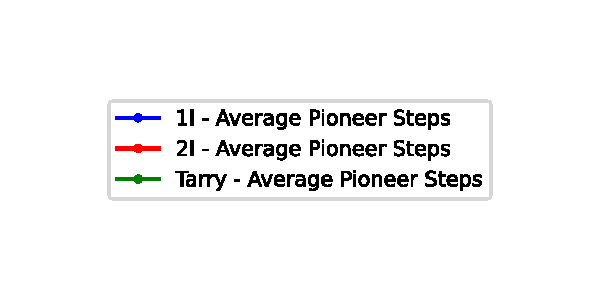
\includegraphics[width=0.5\textwidth]{Cap3/no_comm_steps_legend.pdf} }}
    \newline
    \subfloat[\centering 10x10 Maze]
    {{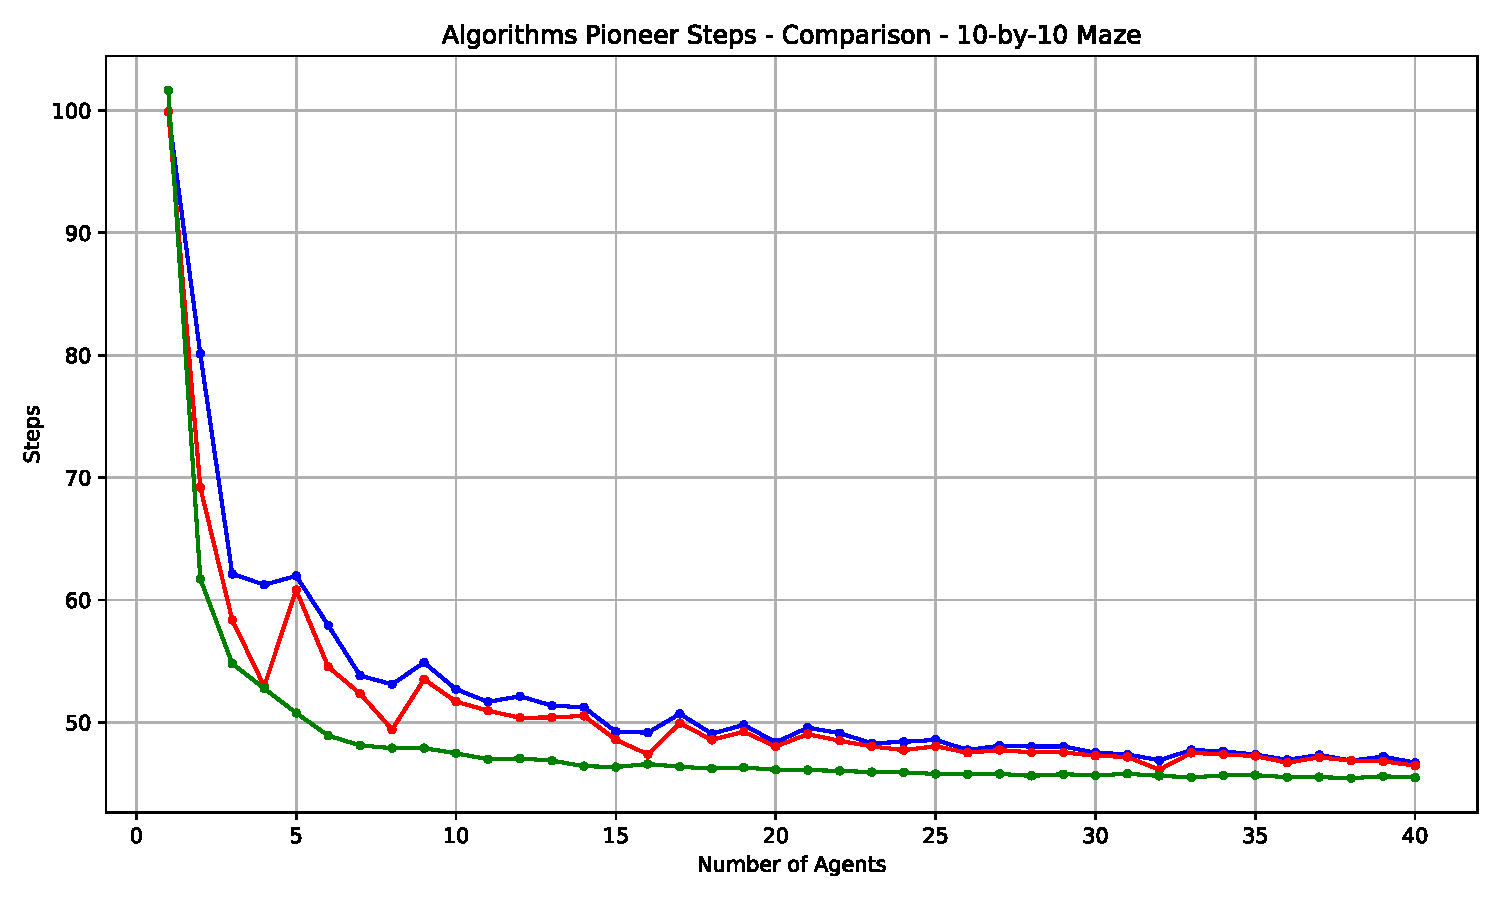
\includegraphics[width=0.45\linewidth]{Cap3/no_comm_steps__10_by_10_maze.pdf} }}
    \qquad
    \subfloat[\centering 20x20 Maze]
    {{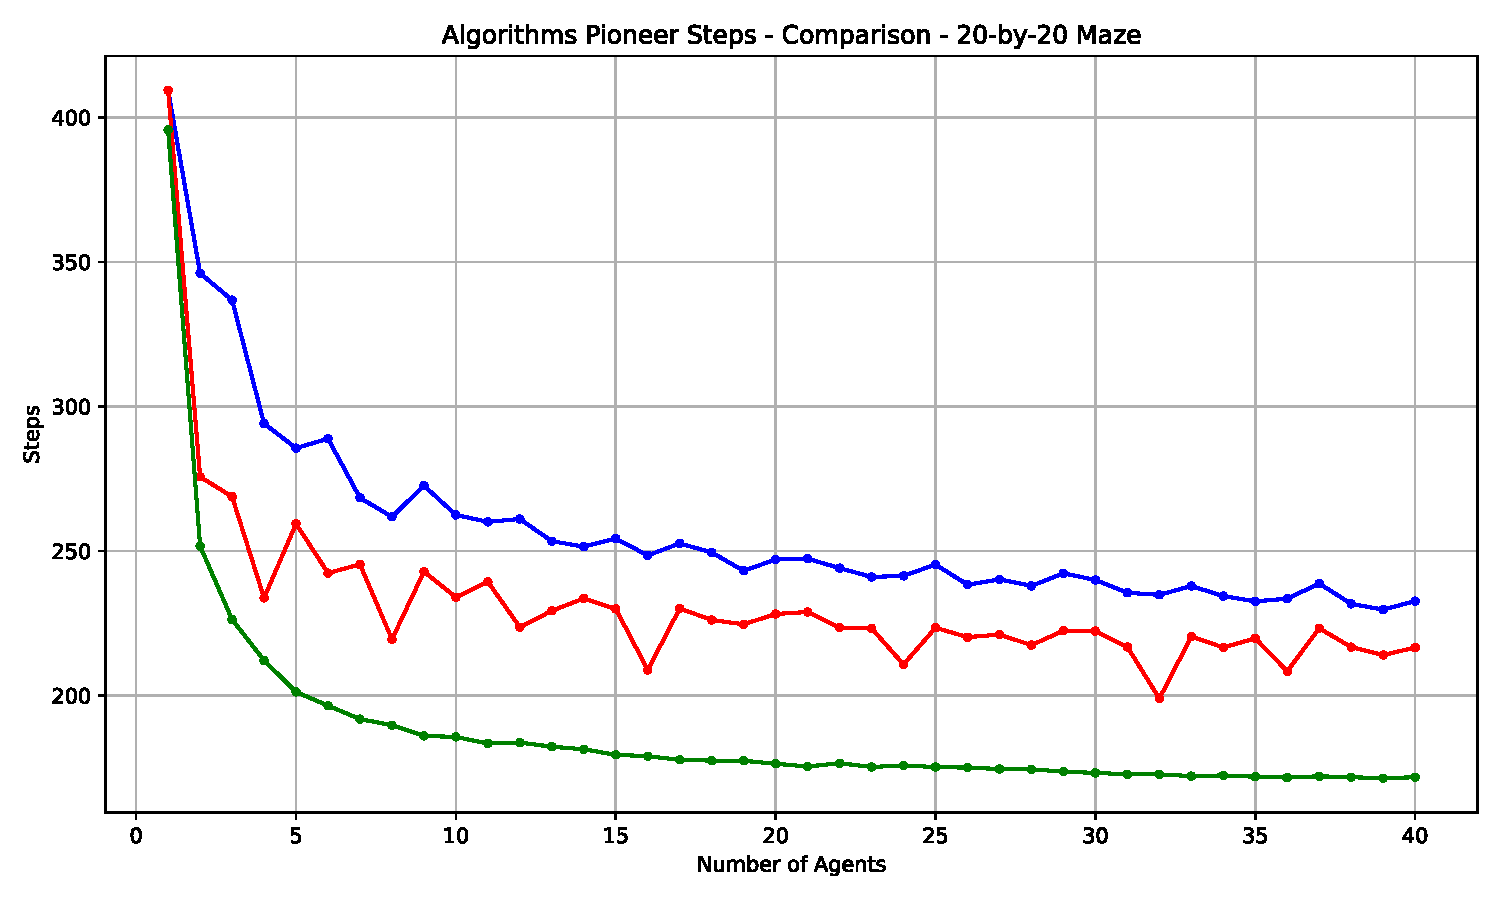
\includegraphics[width=0.45\linewidth]{Cap3/no_comm_steps__20_by_20_maze.pdf} }}
    \newline
    \subfloat[\centering 30x30 Maze]
    {{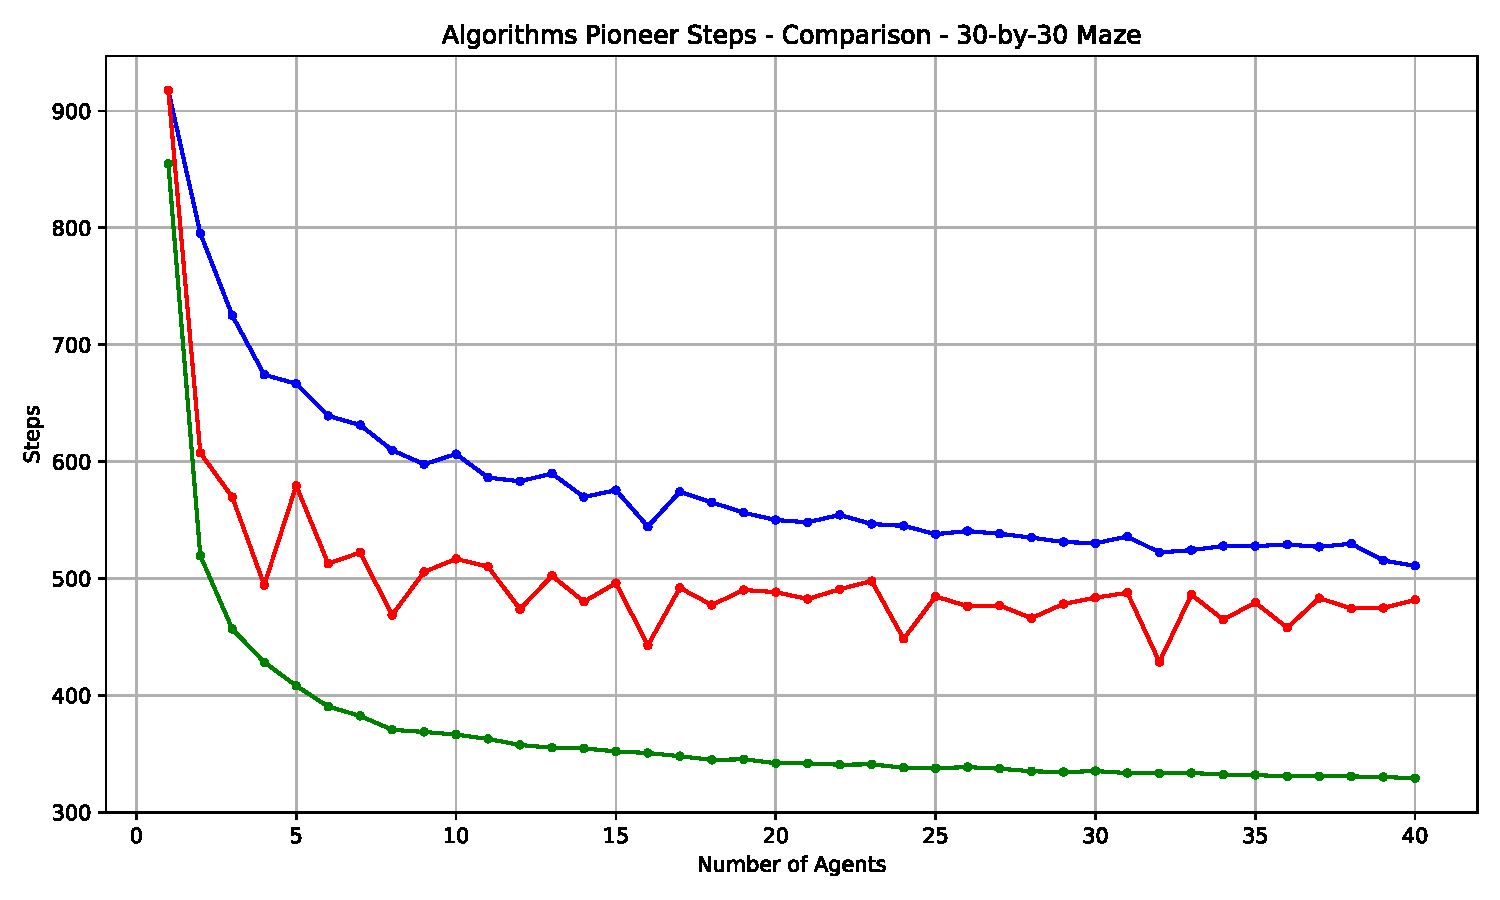
\includegraphics[width=0.45\linewidth]{Cap3/no_comm_steps__30_by_30_maze.pdf} }}
    \qquad
    \subfloat[\centering 40x40 Maze]
    {{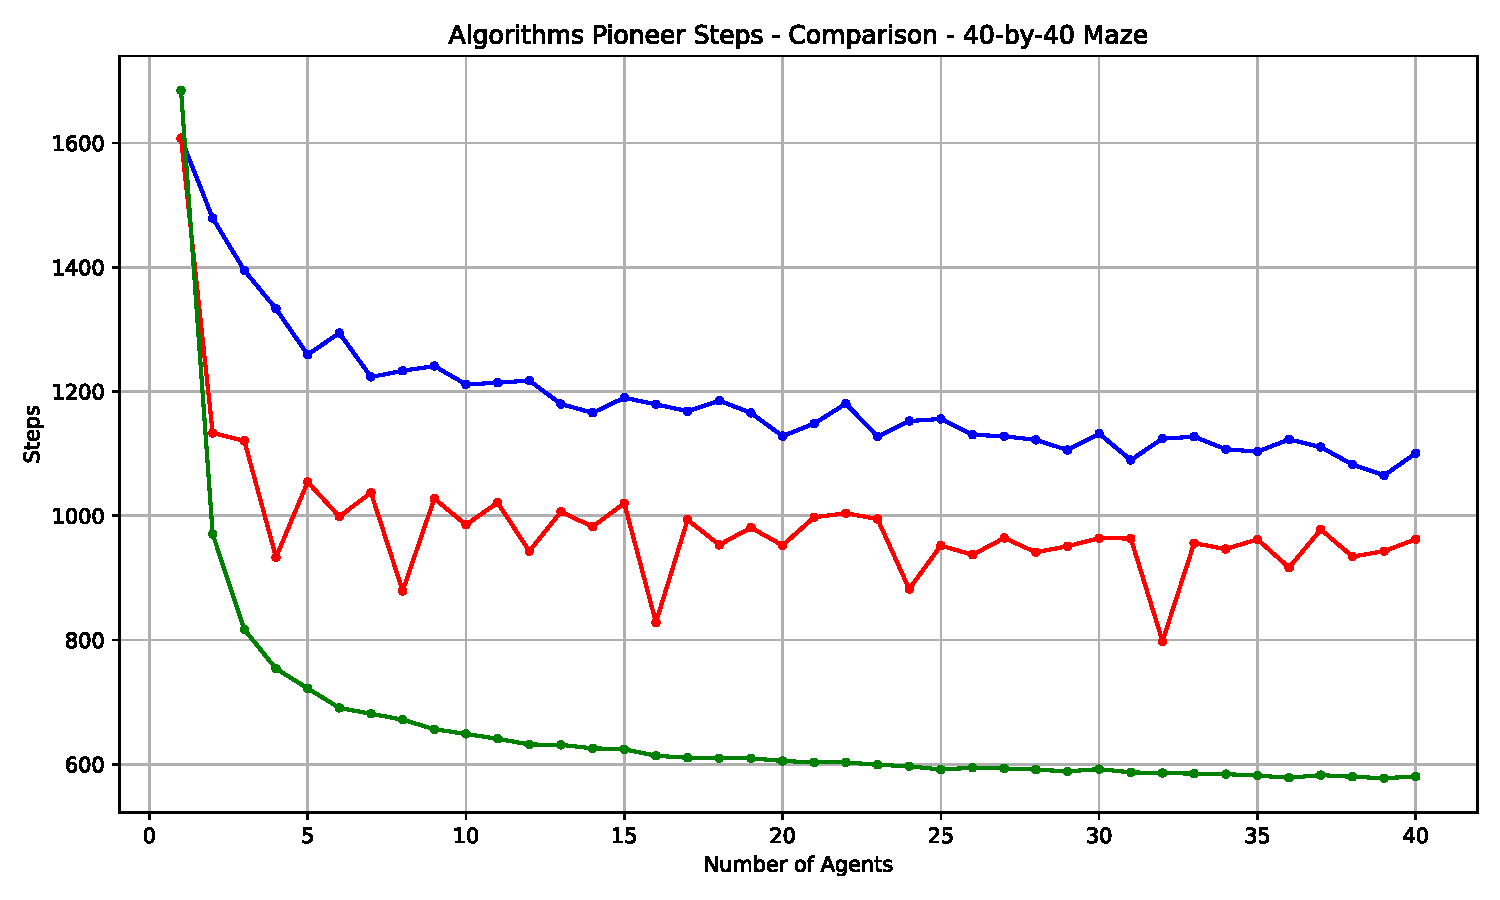
\includegraphics[width=0.45\linewidth]{Cap3/no_comm_steps__40_by_40_maze.pdf} }}
    \caption{Comparison of the pioneer's average steps between our no-communication algorithms and Tarry's algorithm across different sizes of perfect mazes. The subfigures illustrate how algorithm performance scales with maze size.}
    \label{fig_no_comm_steps_all_sizes_maze}
\end{figure}

\begin{figure}[H]
    \centering
    \qquad
    \qquad
    \subfloat[\centering Legend]
    {{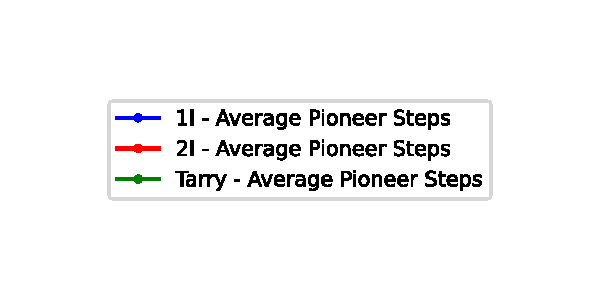
\includegraphics[width=0.5\linewidth]{Cap3/no_comm_steps_legend.pdf} }}
    \newline
    \subfloat[\centering 10x10 Maze]
    {{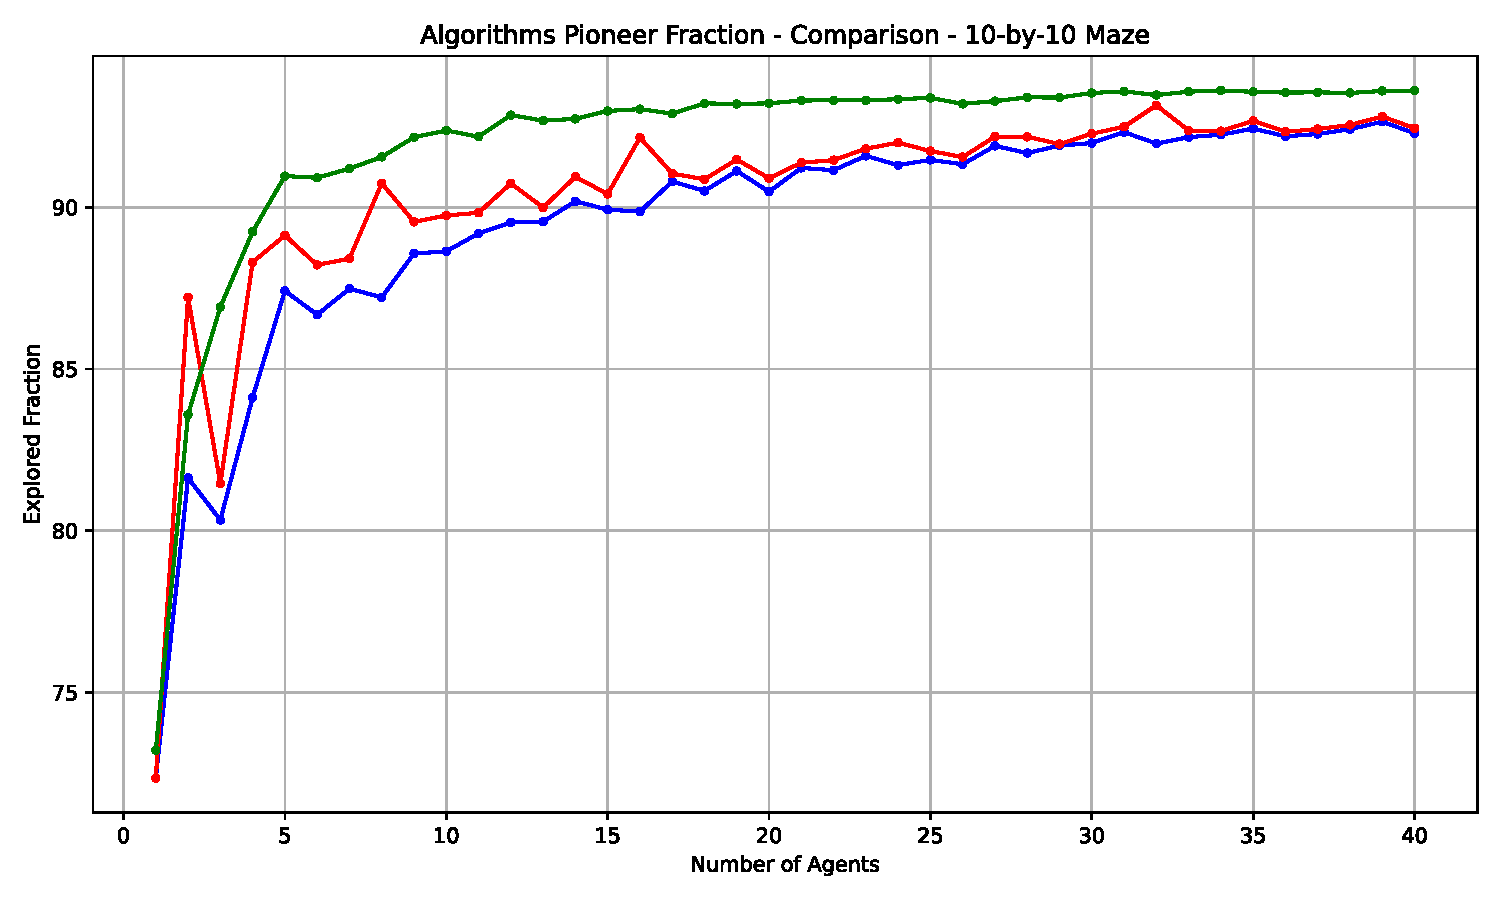
\includegraphics[width=0.45\linewidth]{Cap3/no_comm_fraction__10_by_10_maze.pdf} }}
    \qquad
    \subfloat[\centering 20x20 Maze]
    {{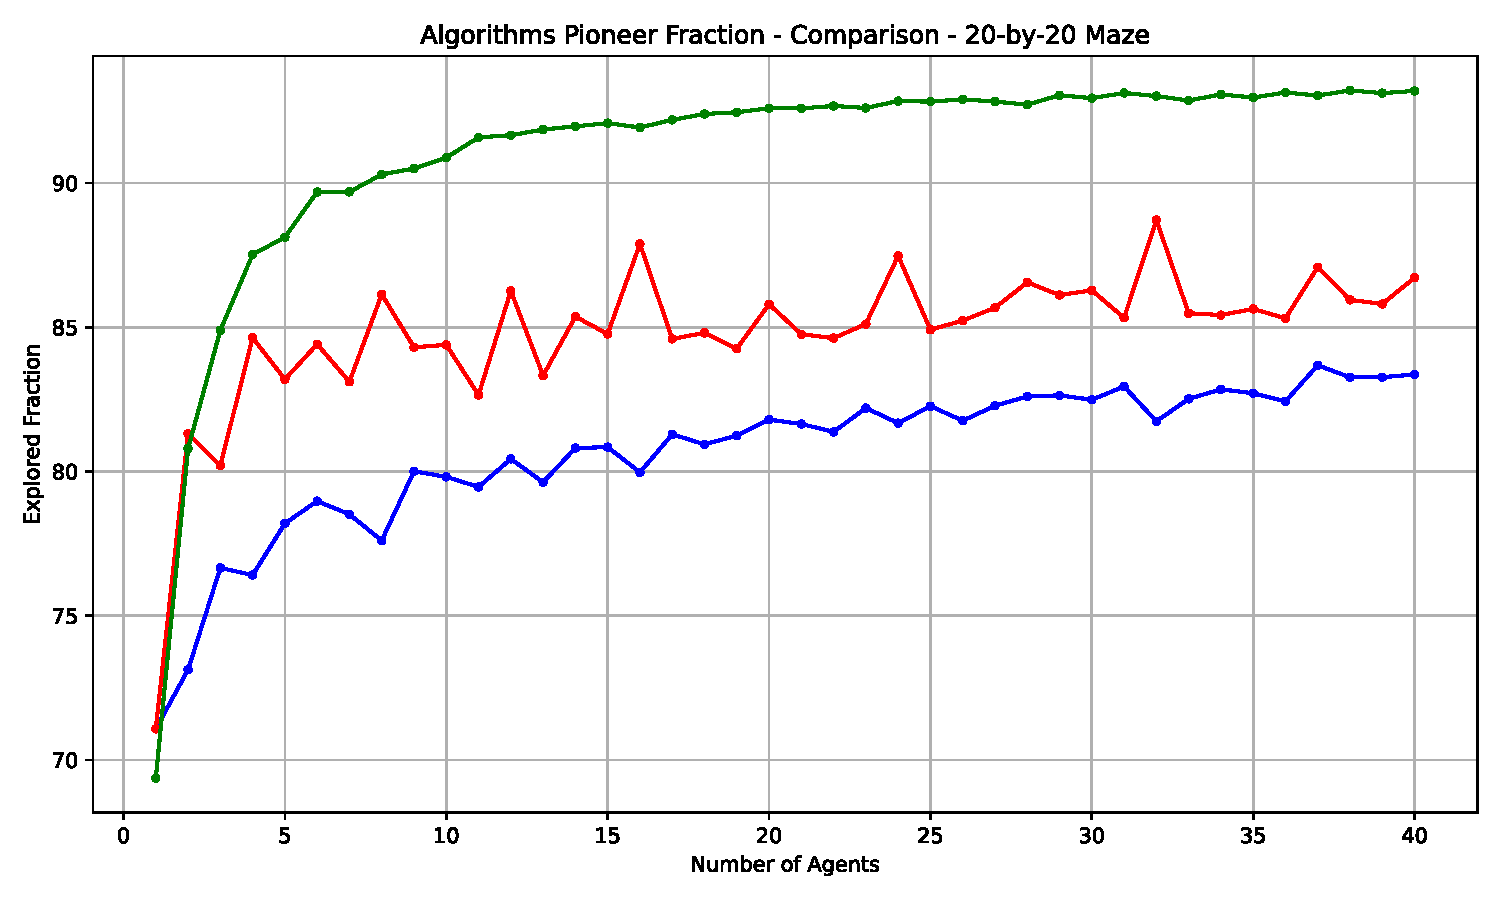
\includegraphics[width=0.45\linewidth]{Cap3/no_comm_fraction__20_by_20_maze.pdf} }}
    \newline
    \subfloat[\centering 30x30 Maze]
    {{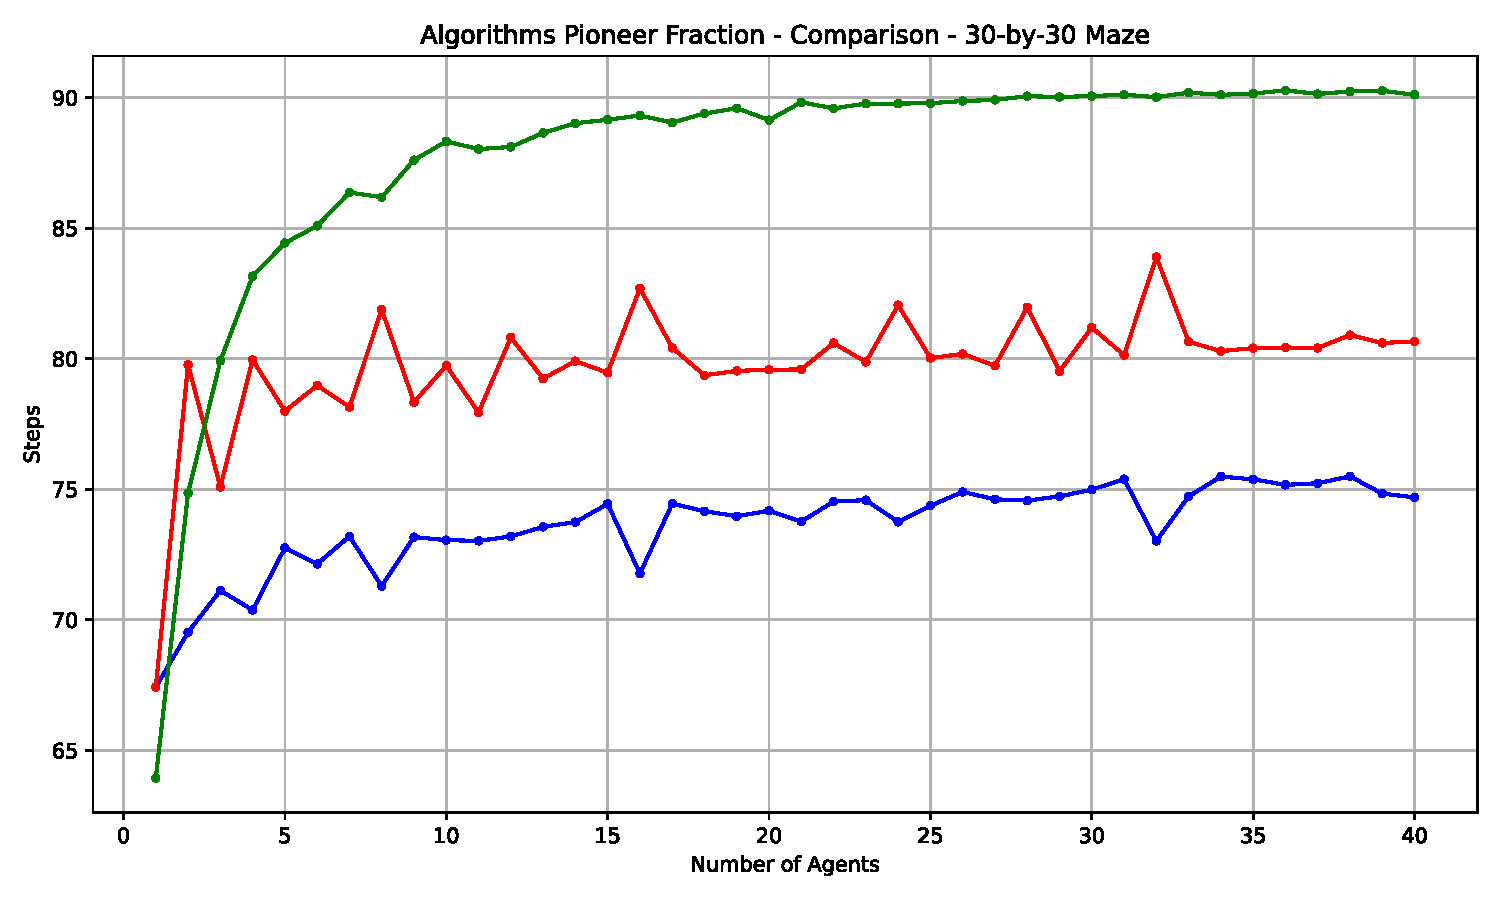
\includegraphics[width=0.45\linewidth]{Cap3/no_comm_fraction__30_by_30_maze.pdf} }}
    \qquad
    \subfloat[\centering 40x40 Maze]
    {{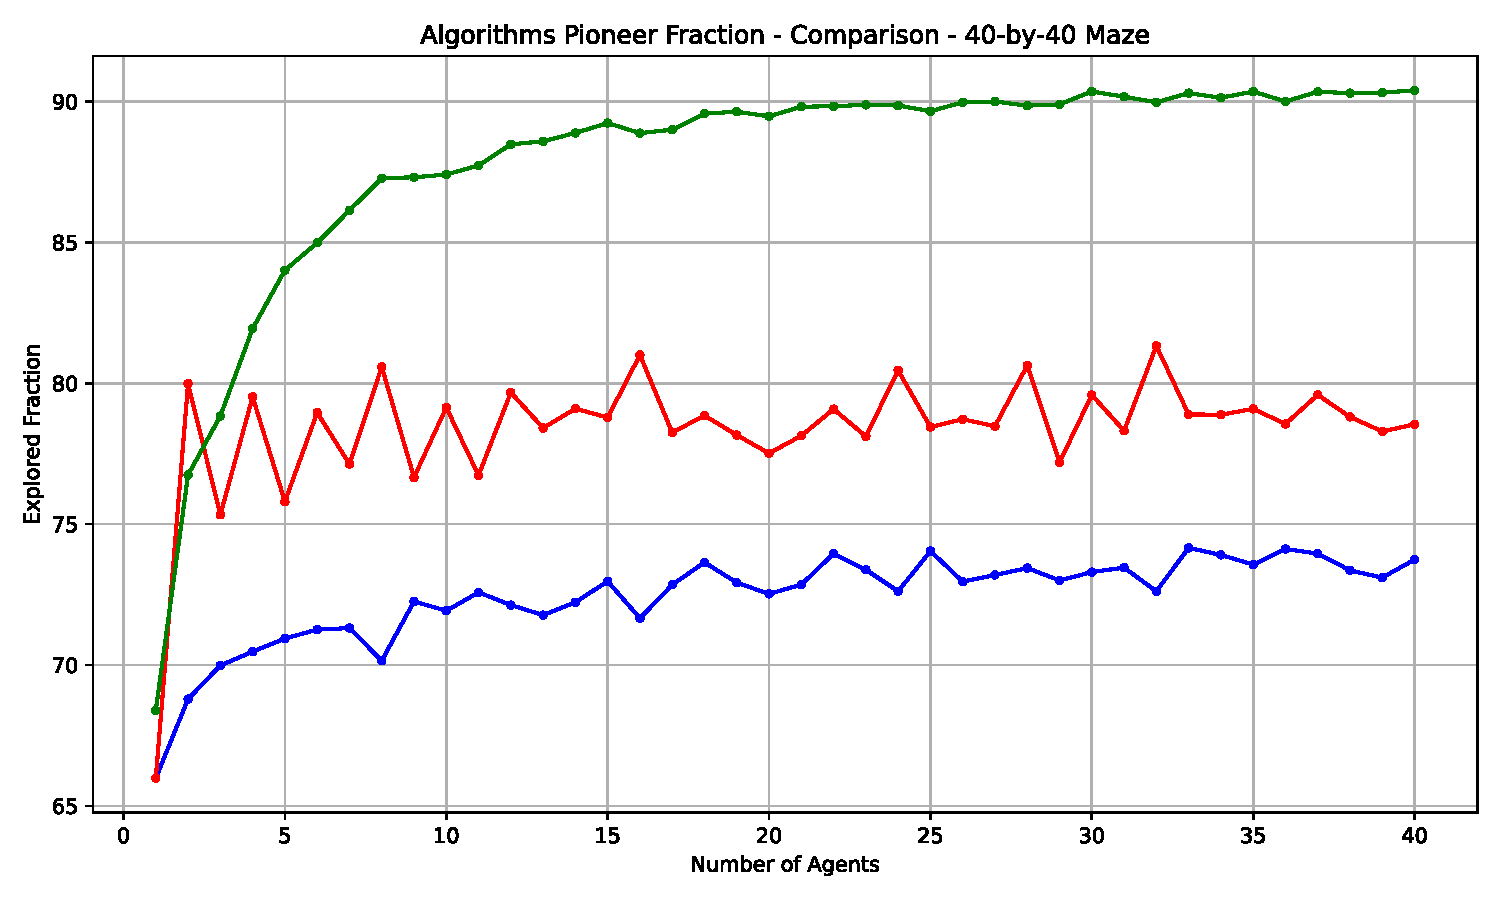
\includegraphics[width=0.45\linewidth]{Cap3/no_comm_fraction__40_by_40_maze.pdf} }}
    \caption{Comparison of the explored fraction achieved by our no-communication algorithms and Tarry's algorithm across different sizes of perfect mazes. The subfigures illustrate how coverage efficiency scales with maze size.}
    \label{fig_no_comm_fraction_all_sizes_maze}
\end{figure}

As this dataset was also used by Rodrigues (2024), and the results shown in Figures \ref{fig_no_comm_steps_all_sizes_maze} and \ref{fig_no_comm_fraction_all_sizes_maze} match his, they confirm the correctness of our new implementation.

The results show that adding more agents helps the pioneer find the goal cell faster, as the average number of steps taken decreases with more agents. This trend eventually levels off at a certain point when there are many agents. The explored fraction behaves similarly, with more agents spreading out quickly and covering more of the maze, though it also stabilizes after a certain number of agents. This outcome is expected, as more agents lead to quicker exploration and better coverage.

In addition to the expected results, the Backward Interval Filling algorithm shows a strange pattern when the number of agents is a power of two, starting from the 20x20 maze size. This matches earlier findings in \cite{Arthur2023}, but it hasn't been fully explored in previous studies. While we recognize the theory suggested by \citen{Arthur2023}, we did not investigate this behavior in detail in our research.

Building on these findings, we compared the performance of our no-communication algorithms with Tarry's algorithm. As expected, both Tarry's algorithm and the Backward Interval Filling variant perform better than the basic version of our algorithm. However, the level of improvement depends on the maze size. In larger mazes, Tarry's algorithm shows a bigger advantage. We conjecture that in smaller mazes, it's possible to quickly find the optimal solution by simply adding more agents. But in larger mazes, communication is crucial for avoiding repeated steps, which we assume significantly enhances Tarry's performance.

\subsection{Random Tree Results} 
\label{subsection_no_comm_random_tree_results}

The results for the random trees of sizes 100, 500, and 1500 nodes are presented in Figure \ref{fig_no_comm_steps_all_sizes_tree}. These sizes were chosen because they effectively represent the trends observed for the metrics without needing to include every possible size. Figure \ref{fig_no_comm_steps_all_sizes_tree} shows the steps taken by the pioneer, while the Figure \ref{fig_no_comm_fraction_all_sizes_tree} shows the explored fraction.

\begin{figure}[H]
    \centering
    \qquad
    \qquad
    \subfloat[\centering Legend]
    {{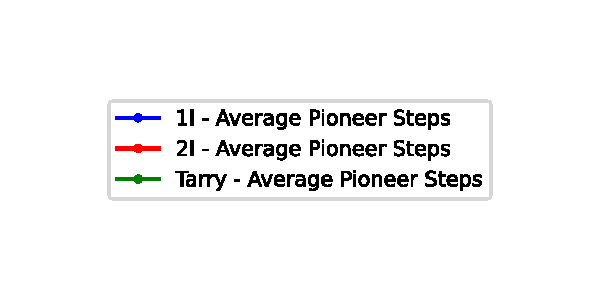
\includegraphics[width=0.5\linewidth]{Cap3/no_comm_steps_legend.pdf} }}
    \newline
    \subfloat[\centering 100-node Tree]
    {{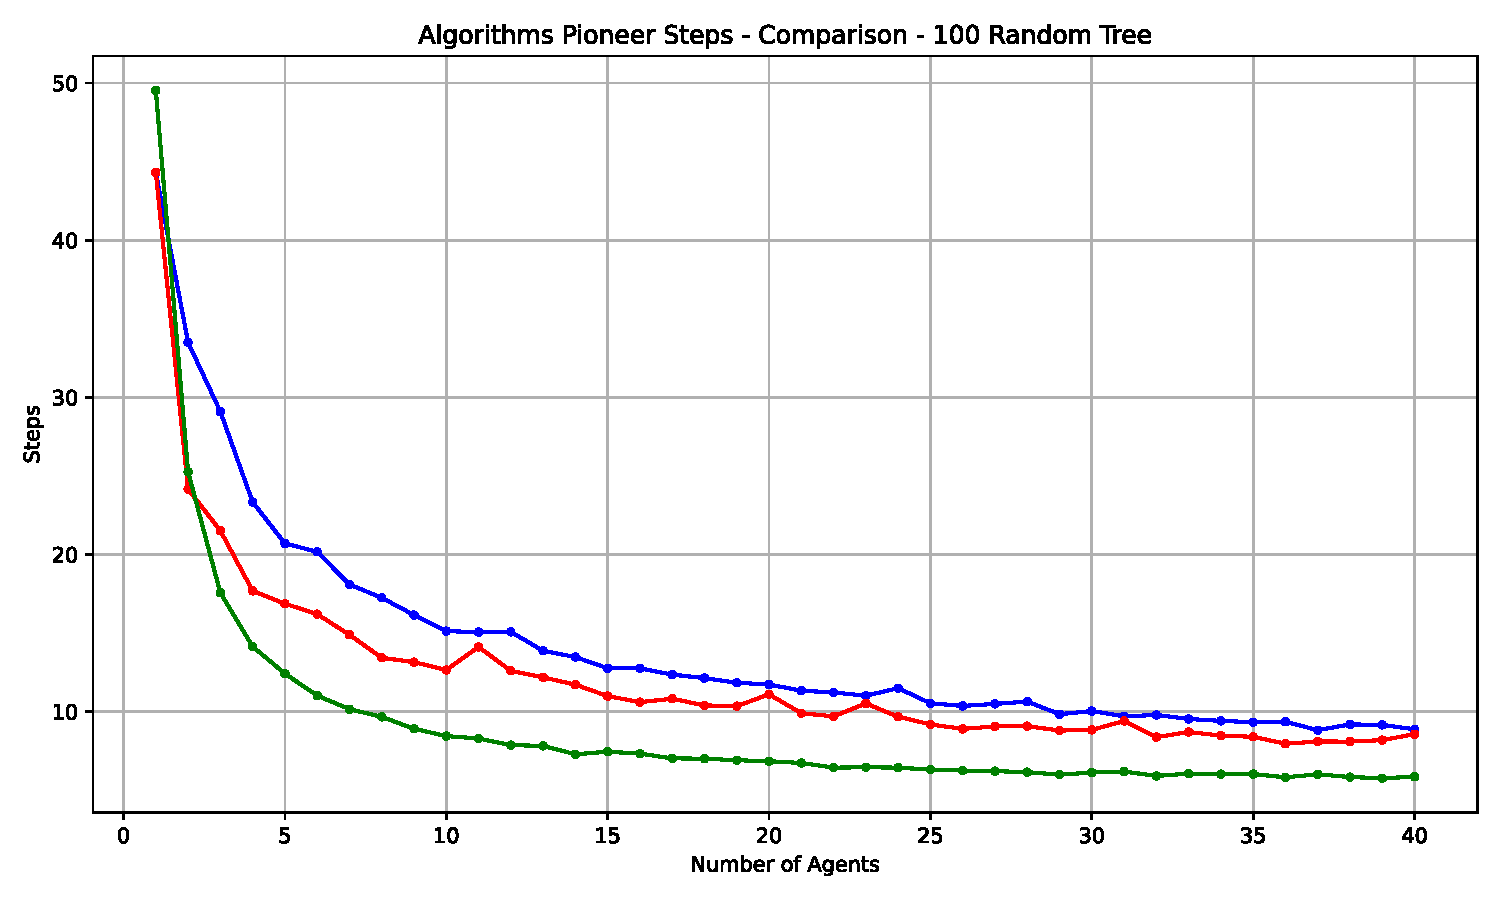
\includegraphics[width=0.45\linewidth]{Cap3/no_comm_steps__100_tree.pdf} }}
    \qquad
    \subfloat[\centering 500-node Tree]
    {{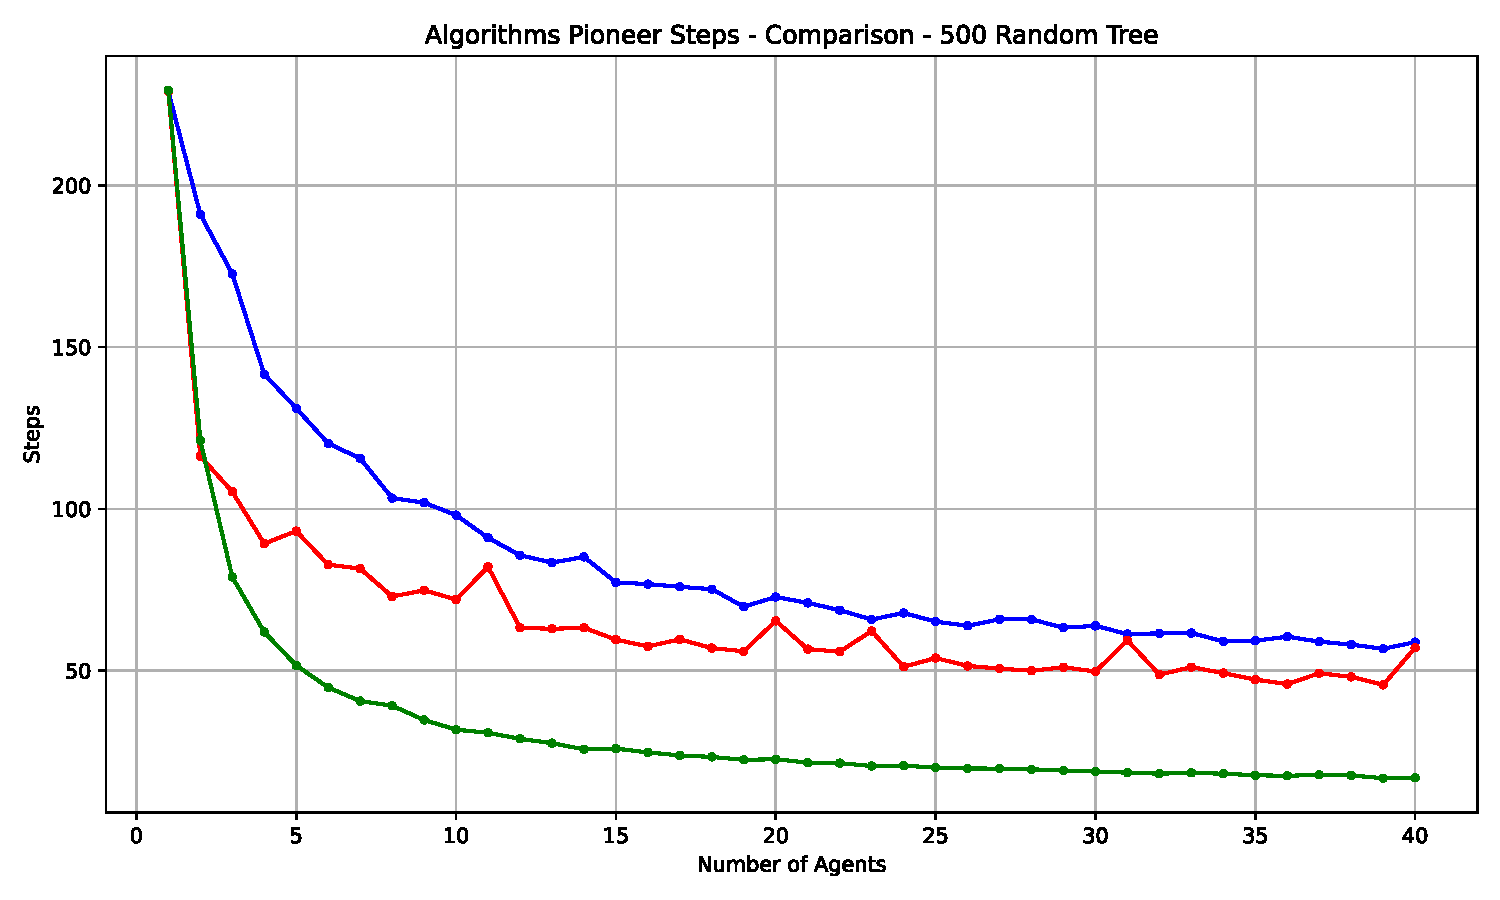
\includegraphics[width=0.45\linewidth]{Cap3/no_comm_steps__500_tree.pdf} }}
    \newline
    \subfloat[\centering 1500-node Tree]
    {{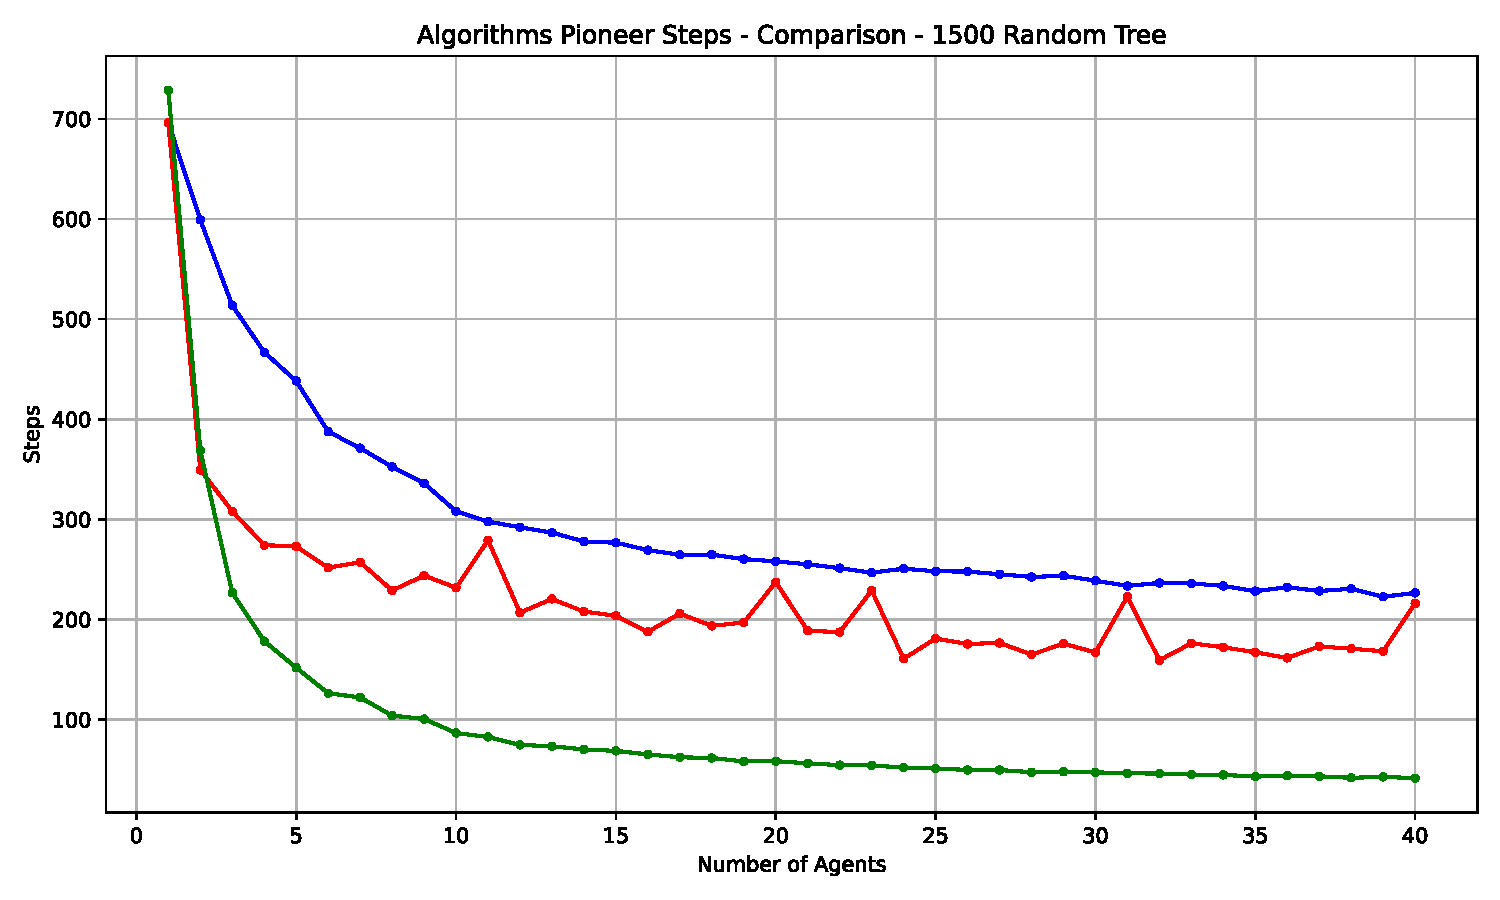
\includegraphics[width=0.45\linewidth]{Cap3/no_comm_steps__1500_tree.pdf} }}
    \caption{Comparison of the average steps taken by the pioneer across different no-communication algorithms and Tarry's algorithm for various sizes of random trees. The subfigures illustrate how algorithm performance varies with tree sizes.}
    \label{fig_no_comm_steps_all_sizes_tree}
\end{figure}

\begin{figure}[H]
    \centering
    \qquad
    \qquad
    \subfloat[\centering Legend]
    {{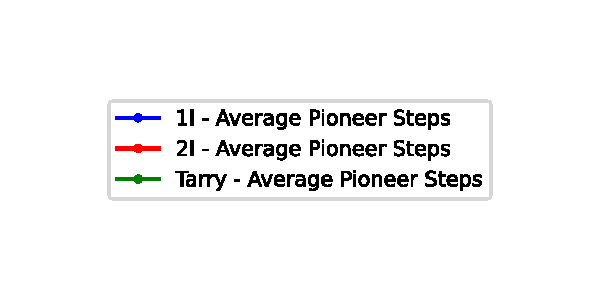
\includegraphics[width=0.5\linewidth]{Cap3/no_comm_steps_legend.pdf} }}
    \newline
    \subfloat[\centering 100-node Tree]
    {{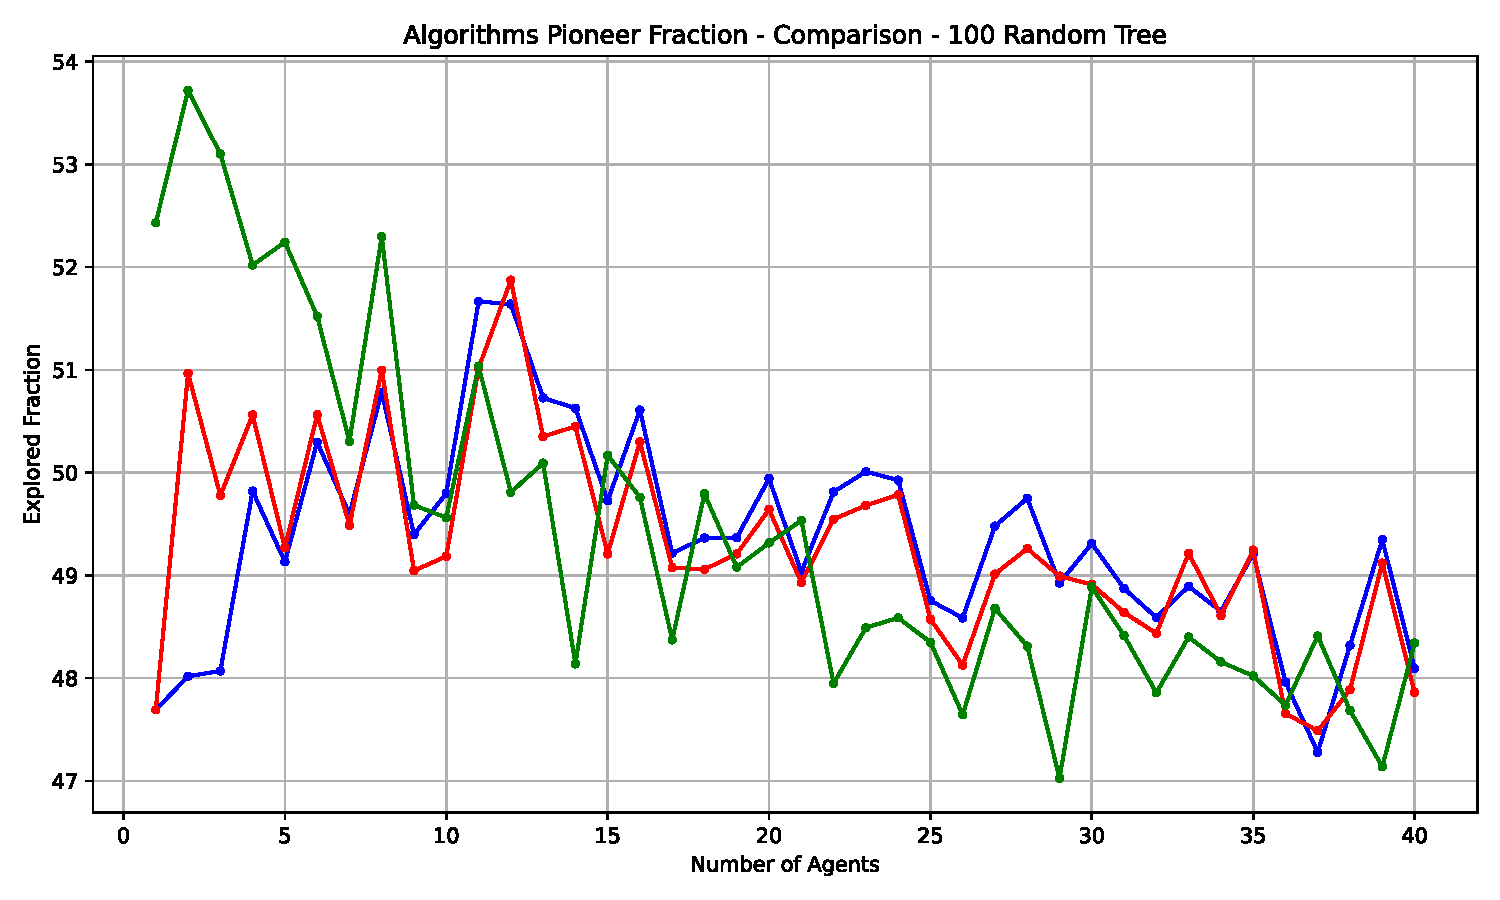
\includegraphics[width=0.45\linewidth]{Cap3/no_comm_fraction__100_tree.pdf} }}
    \qquad
    \subfloat[\centering 500-node Tree]
    {{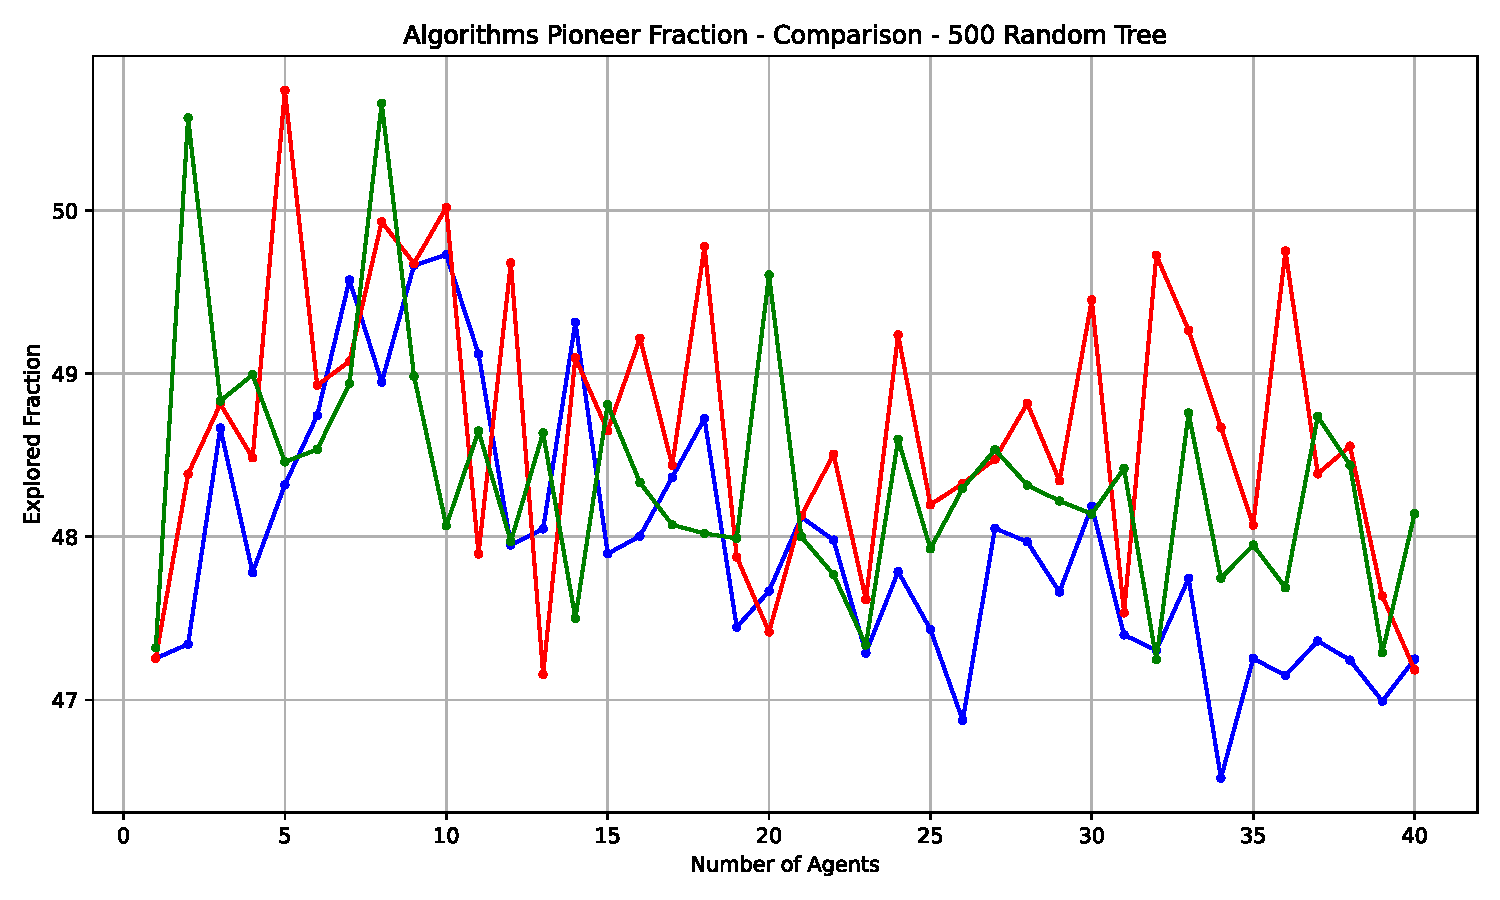
\includegraphics[width=0.45\linewidth]{Cap3/no_comm_fraction__500_tree.pdf} }}
    \newline
    \subfloat[\centering 1500-node Tree]
    {{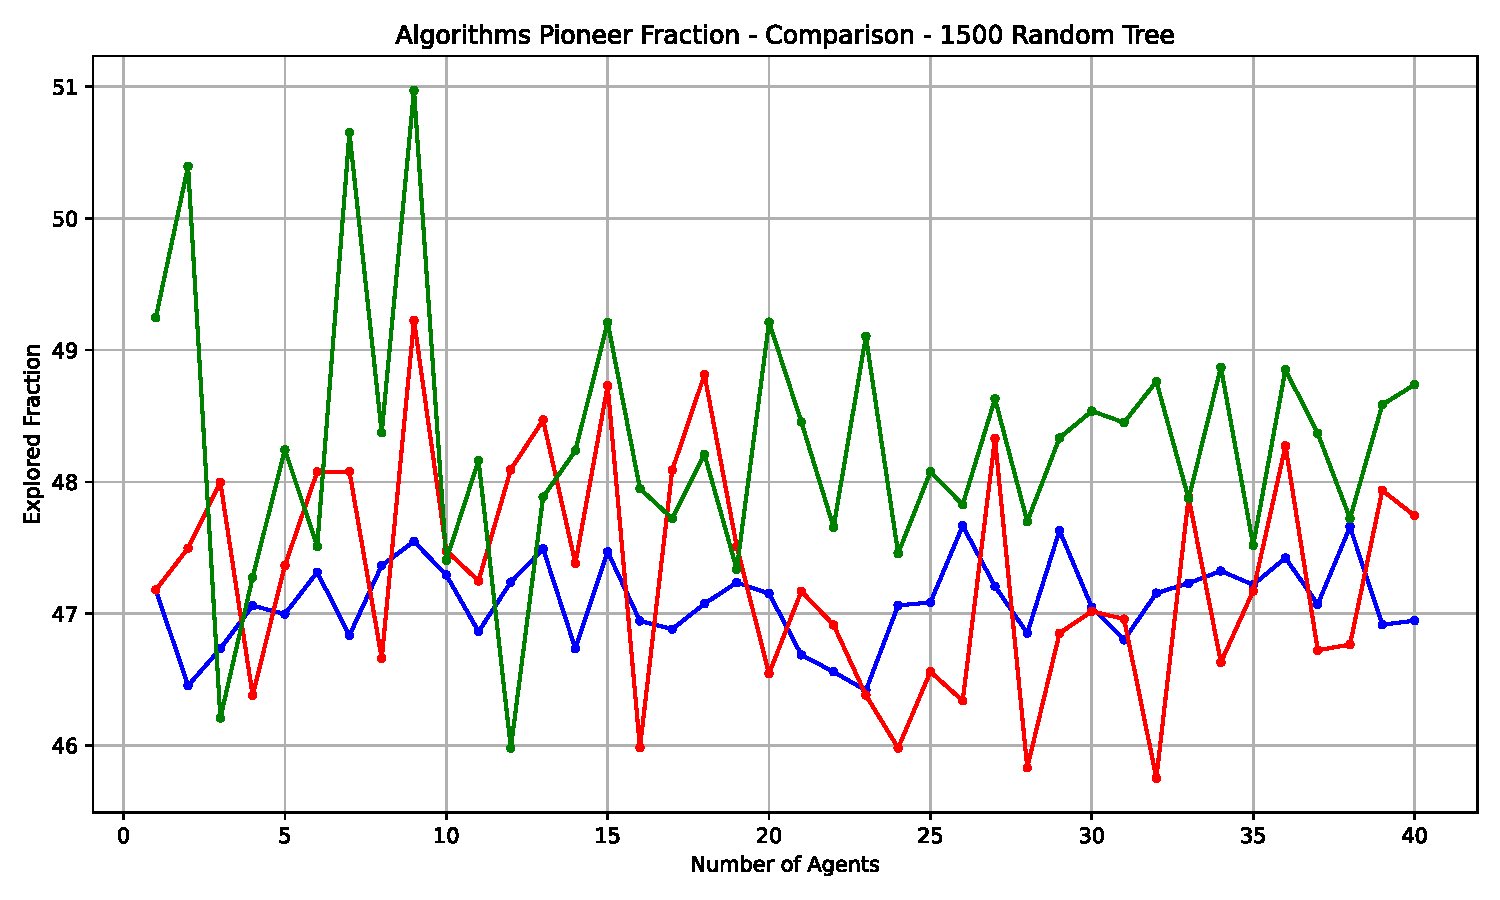
\includegraphics[width=0.45\linewidth]{Cap3/no_comm_fraction__1500_tree.pdf} }}
    \caption{Comparison of the explored fraction achieved by the pioneer across different no-communication algorithms and Tarry's algorithm for various sizes of random trees. The subfigures illustrate how coverage efficiency varies with tree sizes.}
    \label{fig_no_comm_fraction_all_sizes_tree}
\end{figure}

The results for the random trees confirm that the conclusions from Section \ref{subsection_no_comm_maze_results} still apply. Performance improves with more agents, Tarry's algorithm remains the most efficient, and its advantages increase with size.

Even though the trends hold, it's important to note that Tarry outperforms the Back Filling Interval Variation by approximately 39.6\% and our proposed algorithm by 47.3\% in the 40x40 maze. In contrast, in the 1500-node trees, Tarry shows a substantial improvement, being about 81.7\% better than our proposed algorithm and 80.8\% better than the Back Filling Interval Variation. This demonstrates the significant impact of dataset characteristics on the relative performance of our no-communication algorithms.

Referring to Figure \ref{fig_no_comm_fraction_all_sizes_tree}, the results differ from expectations, as the plots are noisy and don't show a clear pattern where Tarry's algorithm consistently explores a larger fraction. Previously, the explored fraction increased with the number of agents, but that trend isn't evident here, as all the algorithms are around the same values with little difference regardless of the number of agents.

This difference arises from the dataset characteristics. In deep trees like Perfect Mazes, agents must explore down to the leaf nodes to find the goal, setting a lower limit on the number of steps. In shallower trees like Random Trees, agents can quickly reach leaf nodes, potentially finding the goal earlier regardless of agent count.

As a result, some instances show a very small explored fraction, while others have a higher one, leading to noisy averages. For example, considering Tarry's with 1500 nodes and 20 agents, the explored fraction averaged 49.21\% with a standard deviation of 30.07\%, highlighting this variability. This large spread means this metric is not very relevant for this kind of dataset. On the other hand, zero-communication algorithms do not incur on any loss with respect to this metric.

\begin{figure}[H]
    \centering 
    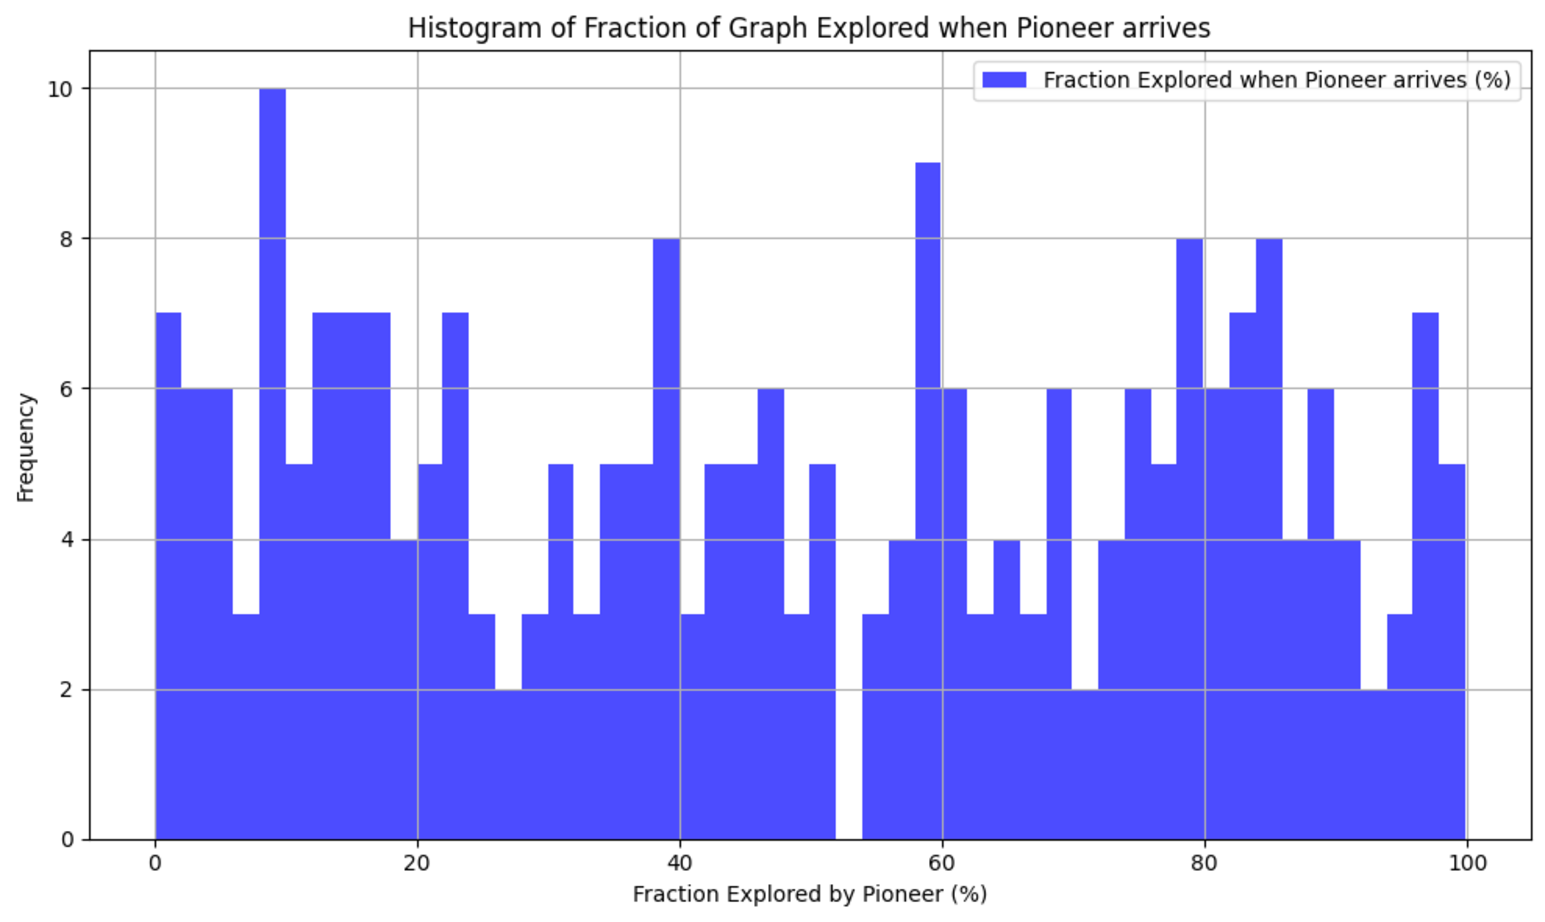
\includegraphics[width=0.7\textwidth]{Cap3/no_comm_fraction_histogram_tree.pdf} 
    \caption{Histogram of explored fractions for random trees with 1500 nodes and 20 agents using Tarry's Algorithm.} 
    \label{fig_no_comm_fraction_histogram_tree}
\end{figure}

As expected, Figure \ref{fig_no_comm_fraction_histogram_tree} shows a fairly uniform distribution in the explored fractions, reflecting the characteristics of the random trees.

\subsection{Barabási-Albert Results} 
\label{subsection_no_comm_barabasi_albert_results}

The results for the Barabási-Albert graphs with 100, 250, 500, and 1000 nodes are shown in Figures \ref{fig_no_comm_steps_all_sizes_barabasi} and \ref{fig_no_comm_fraction_all_sizes_barabasi}. These sizes were selected to capture the overall trends in exploration efficiency while accounting for computational constraints on larger Barabási-Albert graphs. Notably, for the 1000-node graph, the maximum number of agents was limited to 30 instead of the standard 40 due to performance considerations. Figure \ref{fig_no_comm_steps_all_sizes_barabasi} illustrates the average steps taken by the pioneer, while Figure \ref{fig_no_comm_fraction_all_sizes_barabasi} displays the explored fraction achieved.

\begin{figure}[H]
    \centering
    \qquad
    \qquad
    \subfloat[\centering Legend]
    {{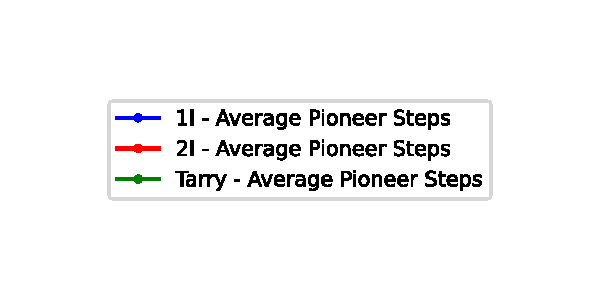
\includegraphics[width=0.5\linewidth]{Cap3/no_comm_steps_legend.pdf} }}
    \newline
    \subfloat[\centering 100-node Barabási-Albert]
    {{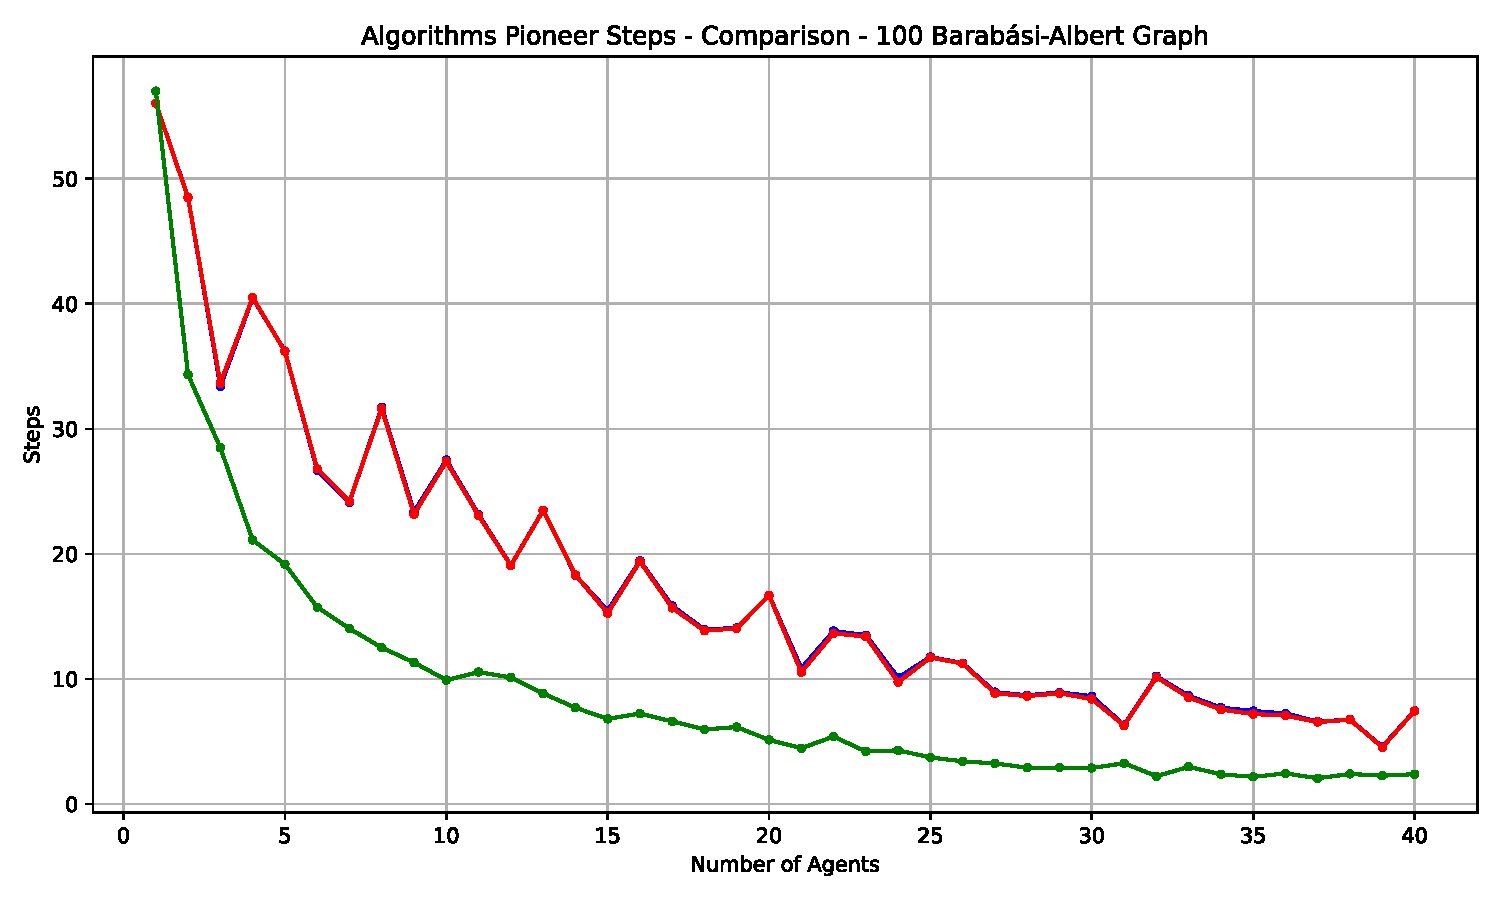
\includegraphics[width=0.45\linewidth]{Cap3/no_comm_steps__100_barabasi.pdf} }}
    \qquad
    \subfloat[\centering 250-node Barabási-Albert]
    {{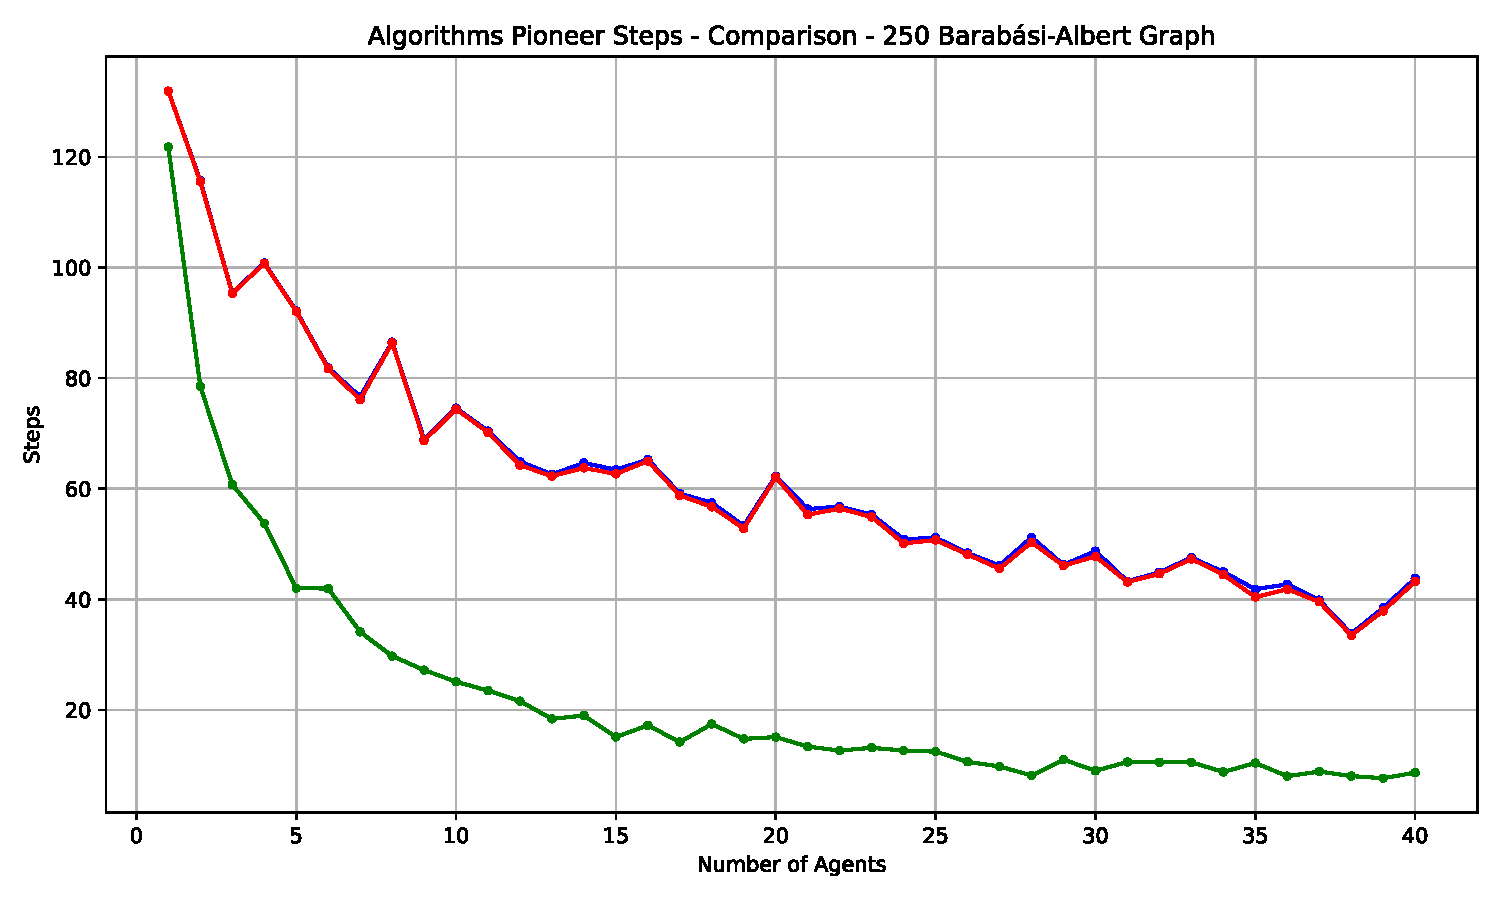
\includegraphics[width=0.45\linewidth]{Cap3/no_comm_steps__250_barabasi.pdf} }}
    \newline
    \subfloat[\centering 500-node Barabási-Albert]
    {{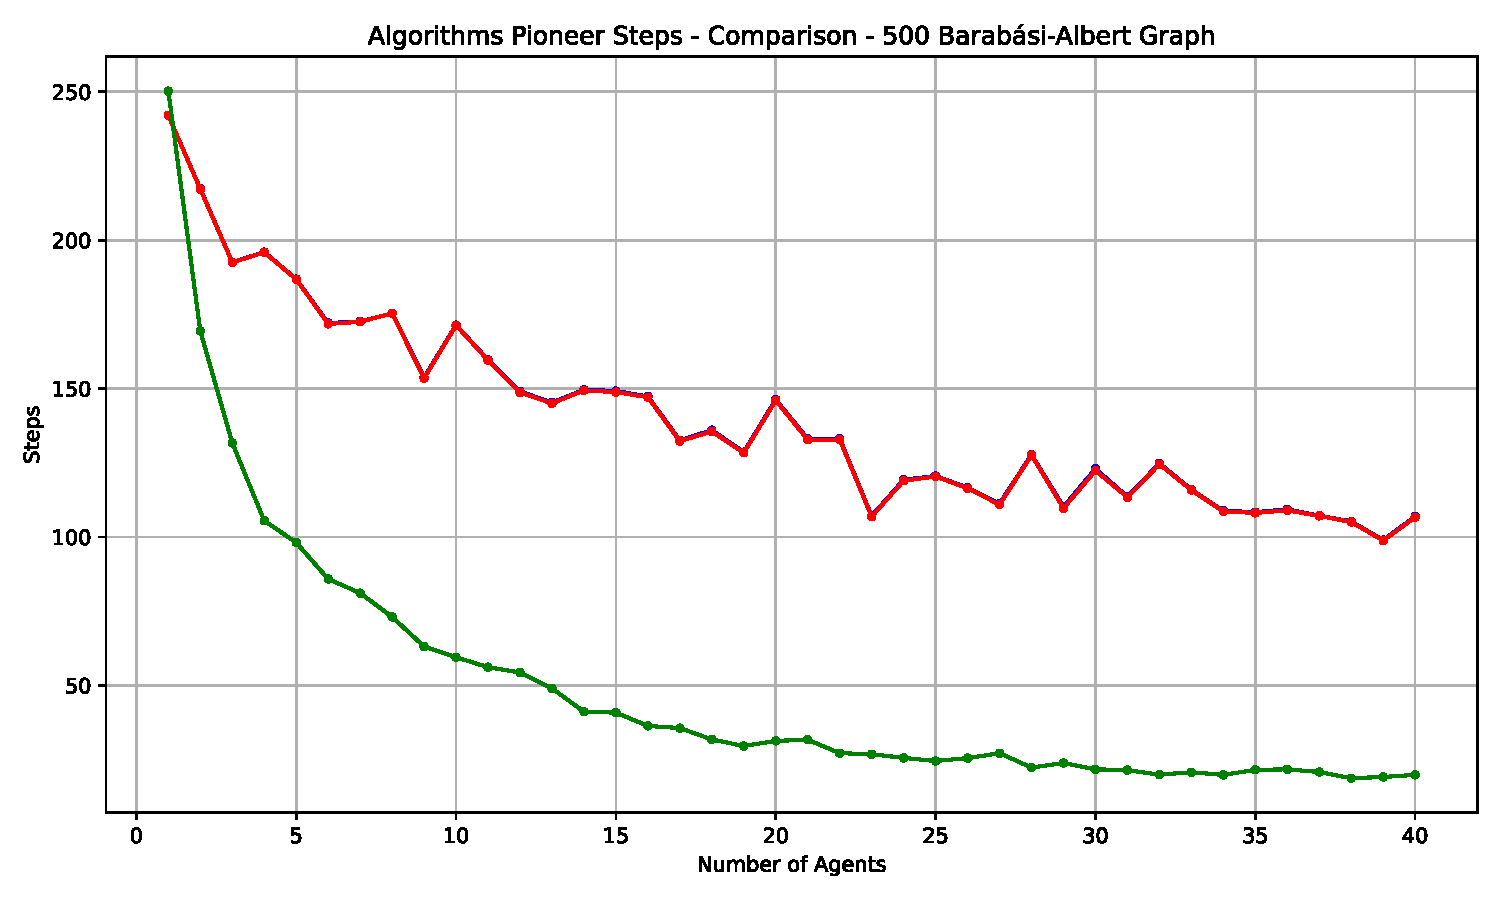
\includegraphics[width=0.45\linewidth]{Cap3/no_comm_steps__500_barabasi.pdf} }}
    \qquad
    \subfloat[\centering 1000-node Barabási-Albert]
    {{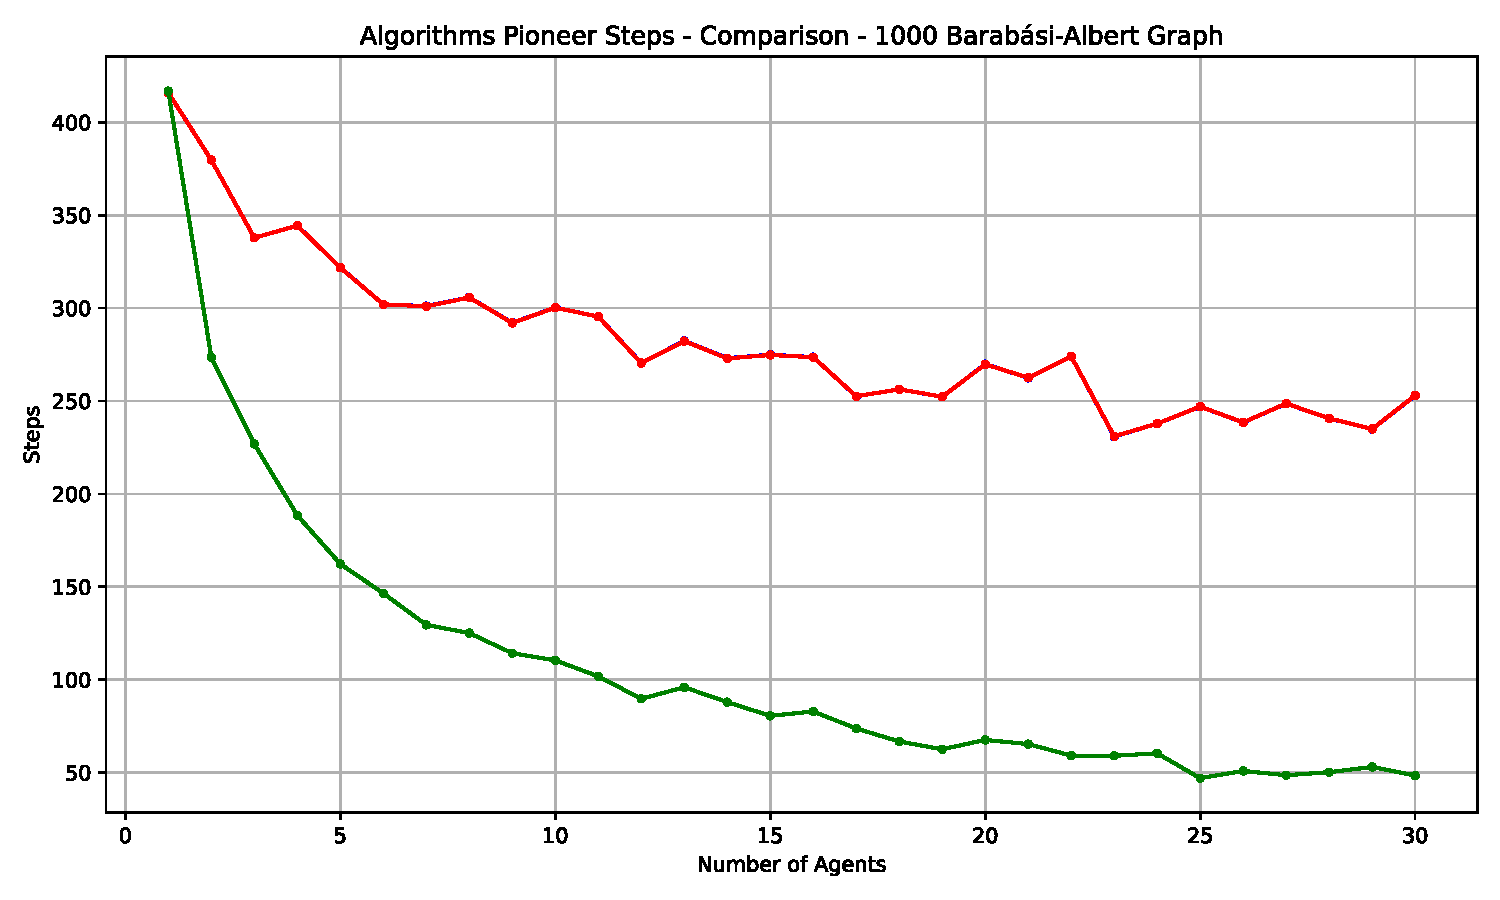
\includegraphics[width=0.45\linewidth]{Cap3/no_comm_steps__1000_barabasi.pdf} }}
    \caption{Comparison of the average steps taken by the pioneer across different no-communication algorithms and Tarry's algorithm for various sizes of Barabási-Albert graphs. The subfigures illustrate how algorithm performance varies with graph sizes.}
    \label{fig_no_comm_steps_all_sizes_barabasi}
\end{figure}

\begin{figure}[H]
    \centering
    \qquad
    \qquad
    \subfloat[\centering Legend]
    {{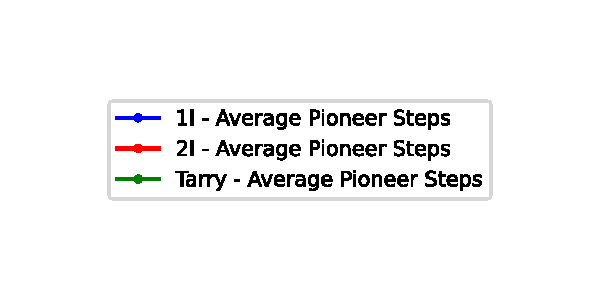
\includegraphics[width=0.5\linewidth]{Cap3/no_comm_steps_legend.pdf} }}
    \newline
    \subfloat[\centering 100-node Barabási-Albert]
    {{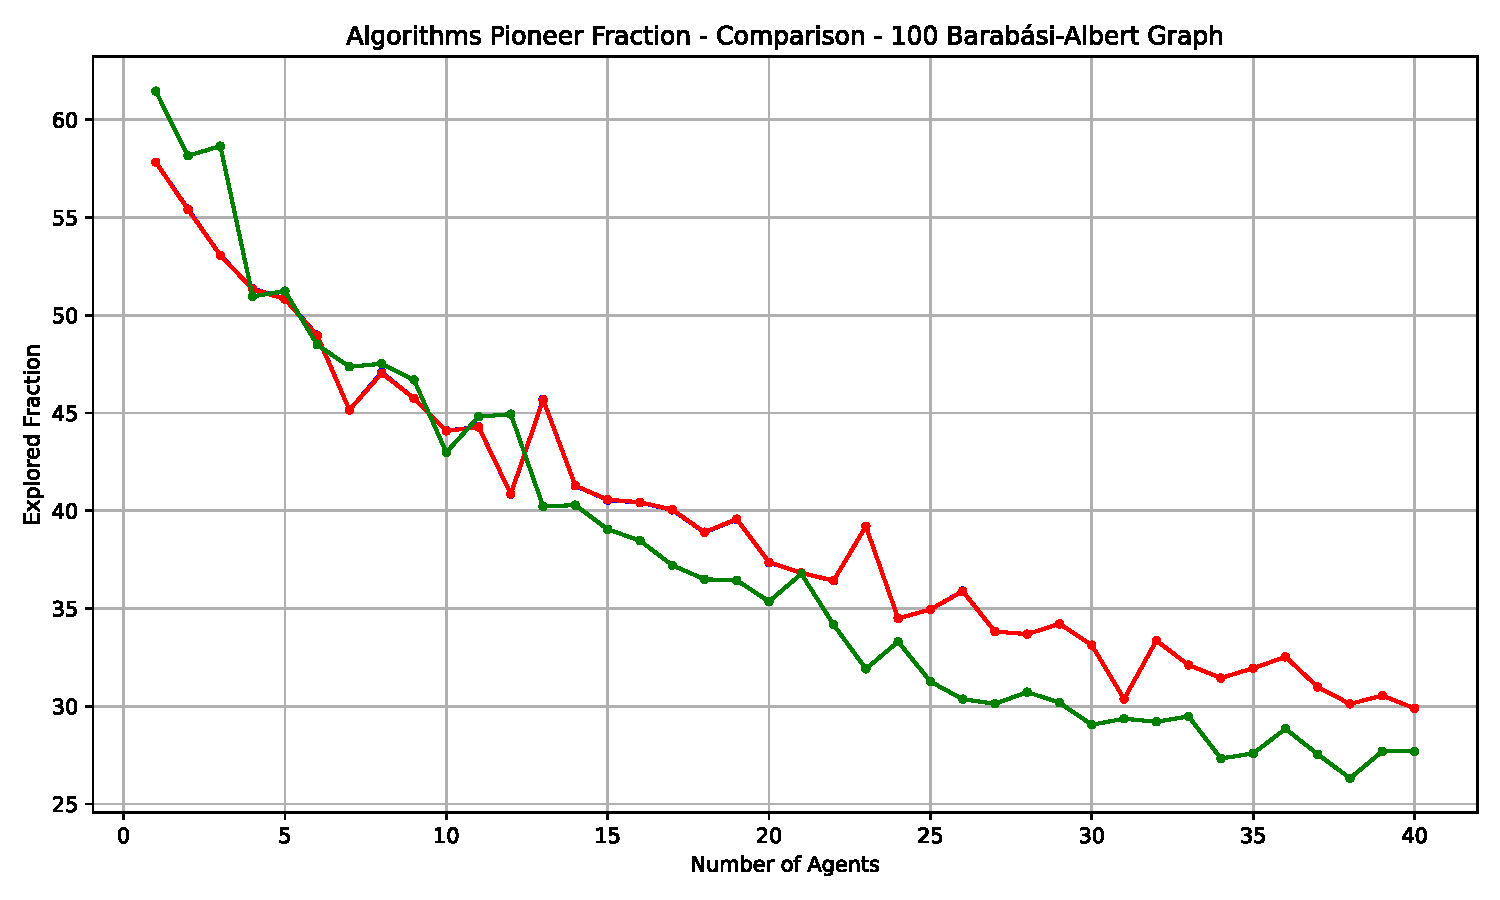
\includegraphics[width=0.45\linewidth]{Cap3/no_comm_fraction__100_barabasi.pdf} }}
    \qquad
    \subfloat[\centering 250-node Barabási-Albert]
    {{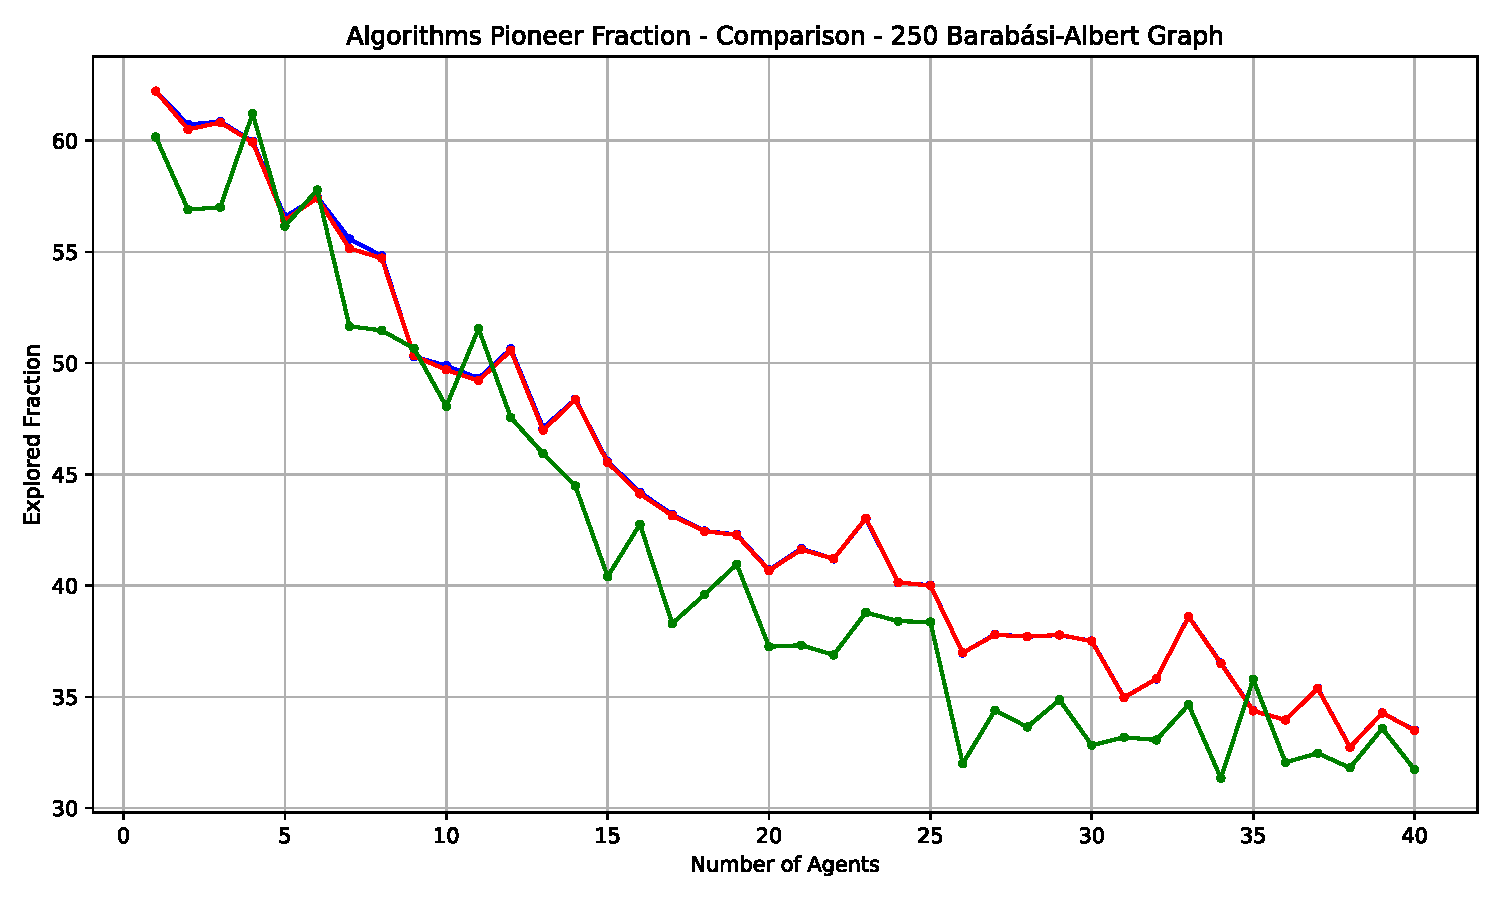
\includegraphics[width=0.45\linewidth]{Cap3/no_comm_fraction__250_barabasi.pdf} }}
    \newline
    \subfloat[\centering 500-node Barabási-Albert]
    {{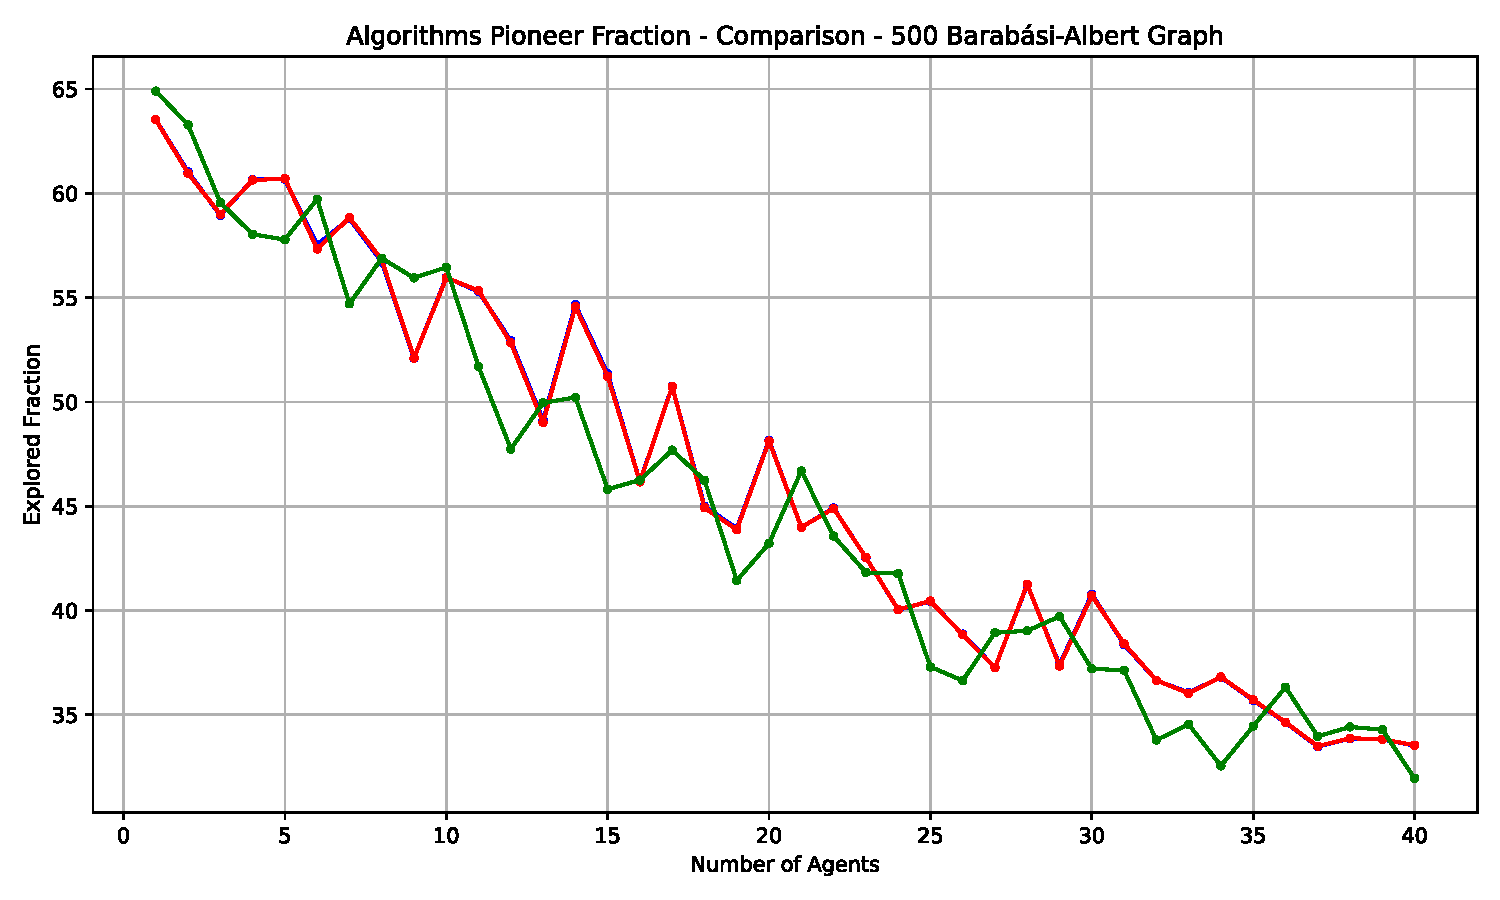
\includegraphics[width=0.45\linewidth]{Cap3/no_comm_fraction__500_barabasi.pdf} }}
    \qquad
    \subfloat[\centering 1000-node Barabási-Albert]
    {{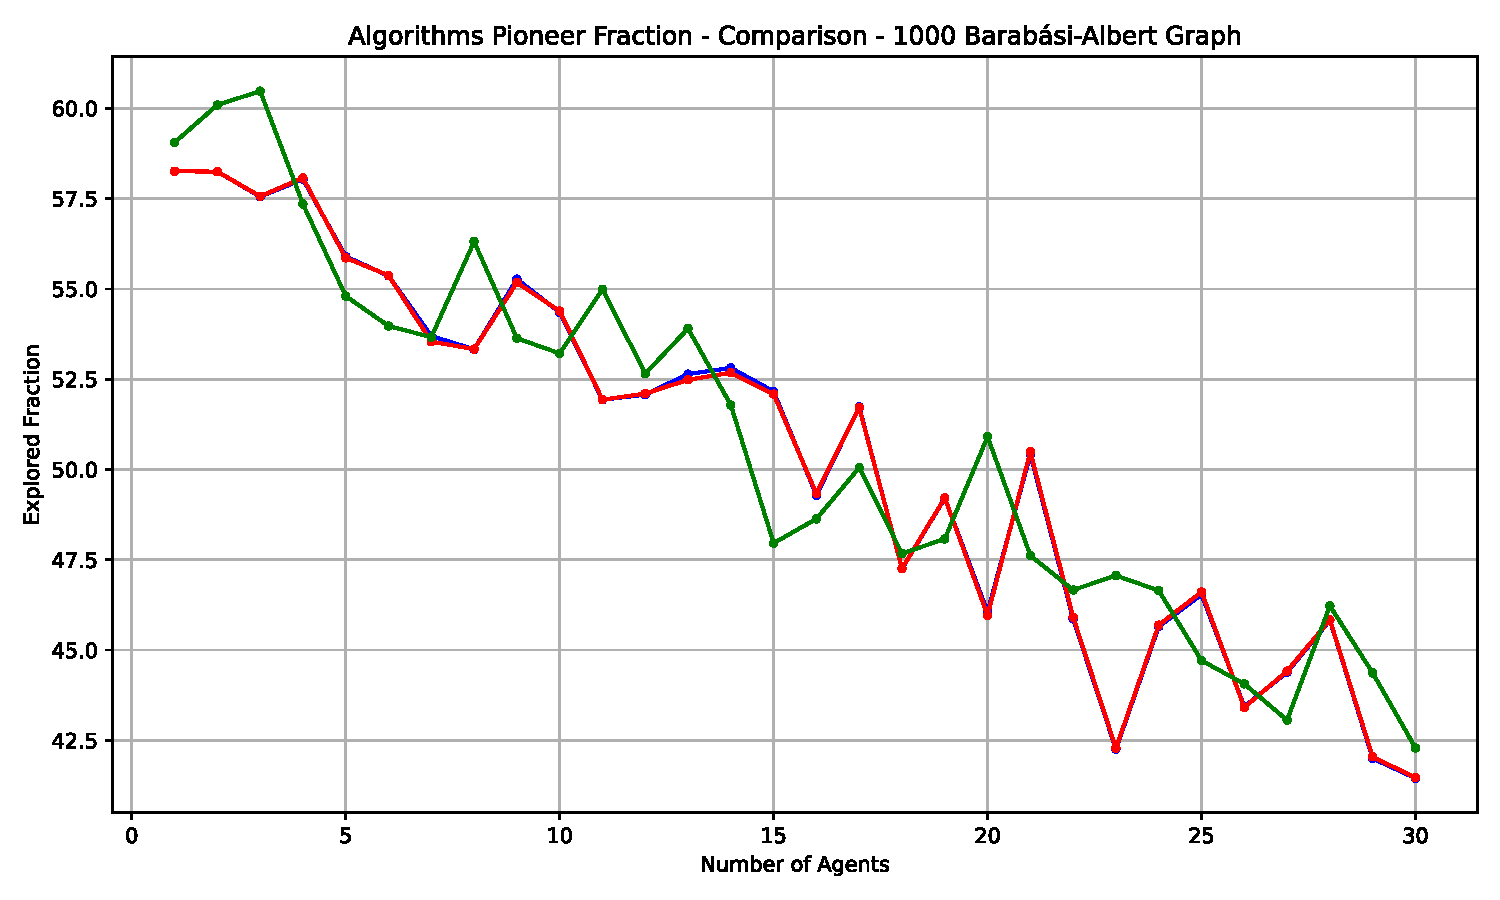
\includegraphics[width=0.45\linewidth]{Cap3/no_comm_fraction__1000_barabasi.pdf} }}
    \caption{Comparison of the explored fraction achieved by the pioneer across different no-communication algorithms and Tarry's algorithm for various sizes of Barabási-Albert graphs. The subfigures illustrate how coverage efficiency varies with graph sizes.}
    \label{fig_no_comm_fraction_all_sizes_barabasi}
\end{figure}

As expected, performance improves with more agents, and Tarry's algorithm remains the most effective approach. However, for this dataset, the Backward Interval Filling algorithm shows no improvement over the basic exploration algorithm. We suspect this is because the Barabási-Albert graphs are highly connected and contain many cycles, leading each agent to form a distinct exploration tree. The same nodes often have significantly different intervals based on the paths taken by each agent. Consequently, each agent completes its initial interval and often reaches the goal before starting a second one.

Unlike the trend observed in Section \ref{subsection_no_comm_maze_results}, the explored fraction decreases with additional agents. This likely occurs because the multiple cycles lead to frequent intersections between agents' exploration trees, adding redundant information. As agents reach the goal quickly, there is less time to explore other parts of the graph.

\section{Tarry's Variants Performance}
\label{section_result_tarry}

\subsection{Metrics for Analysis}
\label{subsection_tarry_metrics}

This section examines the results for Tarry's algorithm and its variants, specifically Tarry Tie-Breaker, Tarry Interval Priority, and Delayed Tarry.

In addition to the previously mentioned metrics in Section \ref{subsection_no_comm_metrics}, this section presents a relative difference in performance compared to the base Tarry algorithm. This approach is particularly useful for interpreting results when the performances of the algorithms are very close on some datasets, as relative values help to better visualize the differences when absolute values are too similar.

\subsection{Perfect Maze Results} 
\label{subsection_tarry_maze_results}

The results for all maze sizes (10x10, 20x20, 30x30, and 40x40) are shown in Figures \ref{fig_tarry_steps_all_sizes_maze}, \ref{fig_tarry_fraction_all_sizes_maze}, and \ref{fig_tarry_steps_relative_all_sizes_maze}, demonstrating the performance of Tarry's algorithm and its variations across different maze dimensions. Figure \ref{fig_tarry_steps_all_sizes_maze} illustrates the number of steps taken by the algorithms, while Figure \ref{fig_tarry_fraction_all_sizes_maze} displays the fraction of the maze explored before reaching the goal, providing insights into exploration efficiency and coverage across maze sizes. Additionally, Figure \ref{fig_tarry_steps_relative_all_sizes_maze} presents the relative difference in pioneer steps compared to the original Tarry's algorithm, helping to better compare the variations, which may show similar behaviors.

\begin{figure}[H]
    \centering
    \qquad
    \qquad
    \subfloat[\centering Legend]
    {{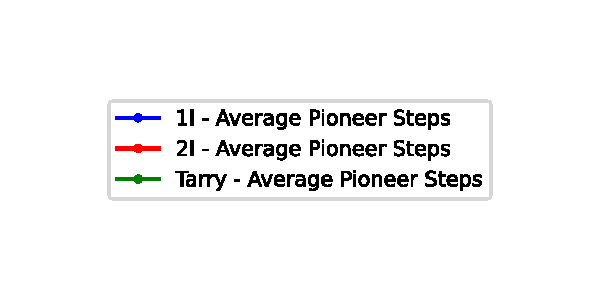
\includegraphics[width=0.5\textwidth]{Cap3/no_comm_steps_legend.pdf} }}
    \newline
    \subfloat[\centering 10x10 Maze]
    {{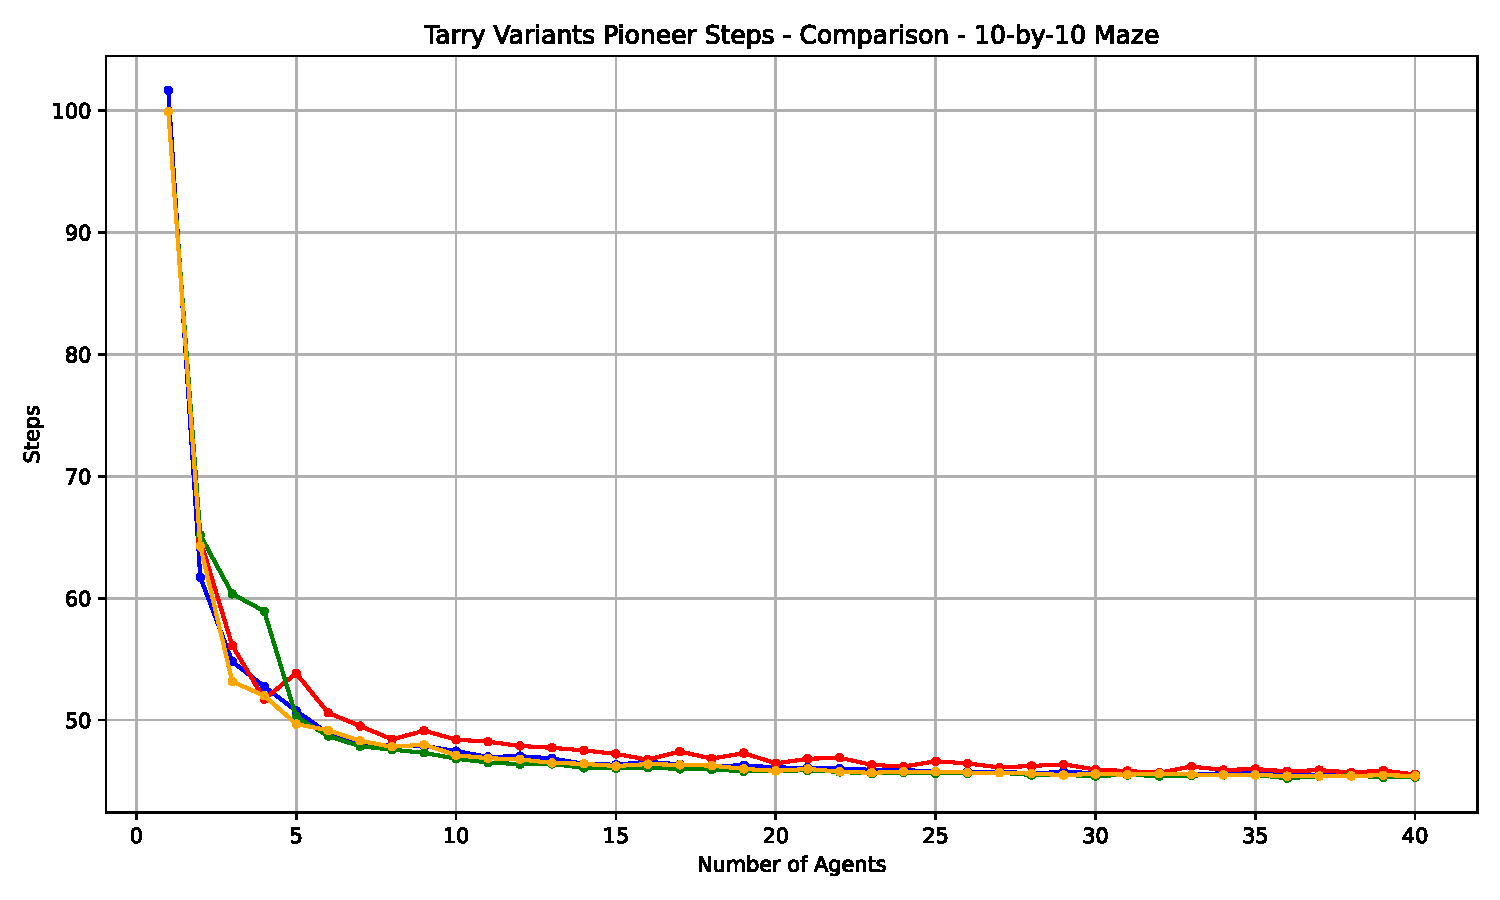
\includegraphics[width=0.45\linewidth]{Cap3/tarry_var_steps__10_by_10_maze.pdf} }}
    \qquad
    \subfloat[\centering 20x20 Maze]
    {{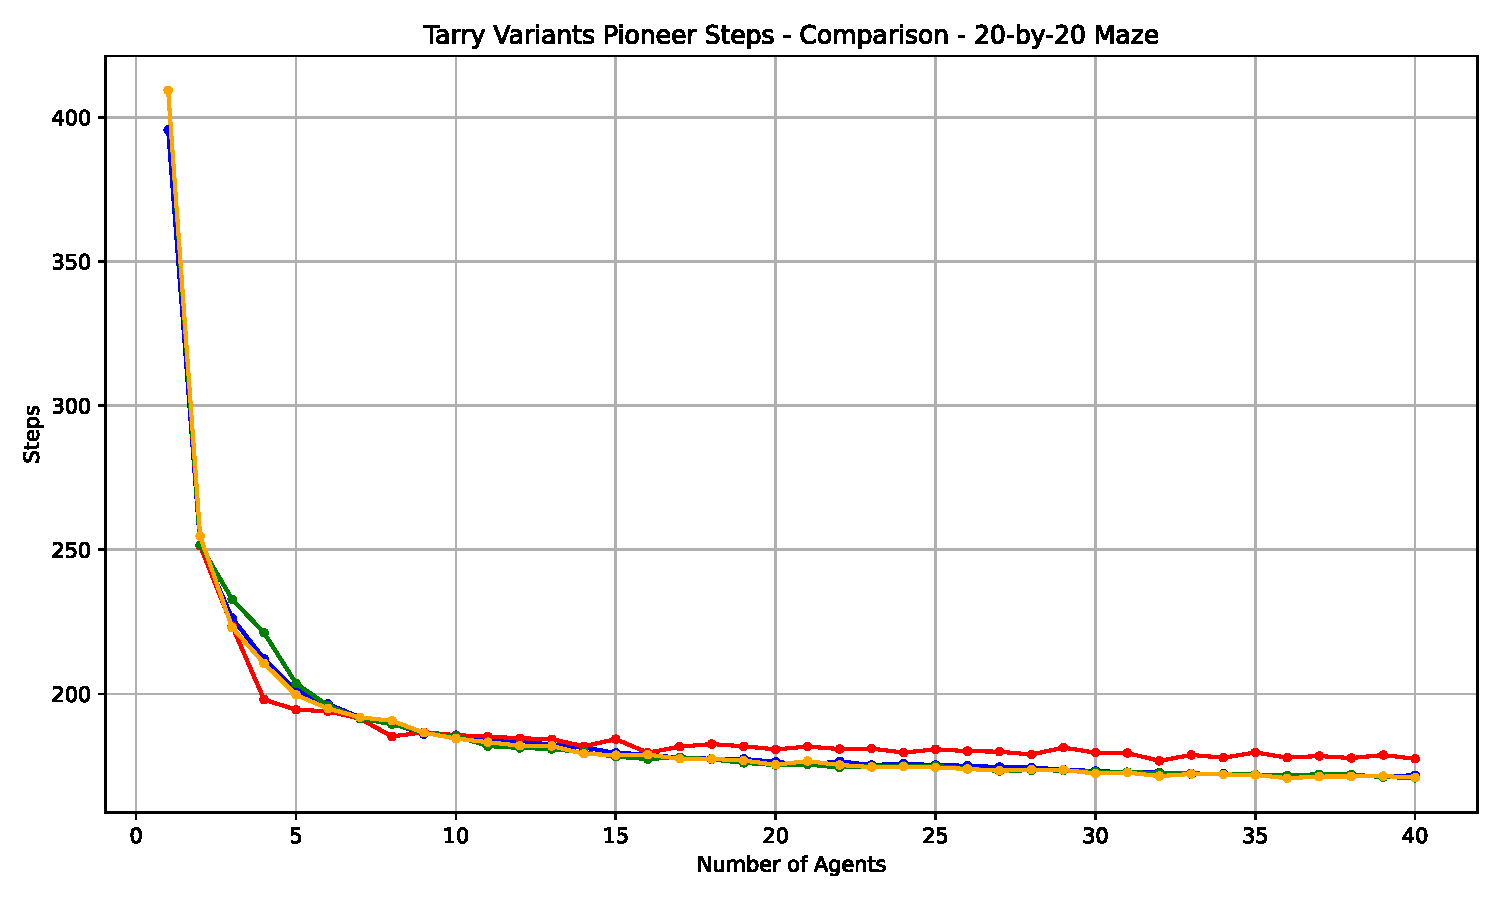
\includegraphics[width=0.45\linewidth]{Cap3/tarry_var_steps__20_by_20_maze.pdf} }}
    \newline
    \subfloat[\centering 30x30 Maze]
    {{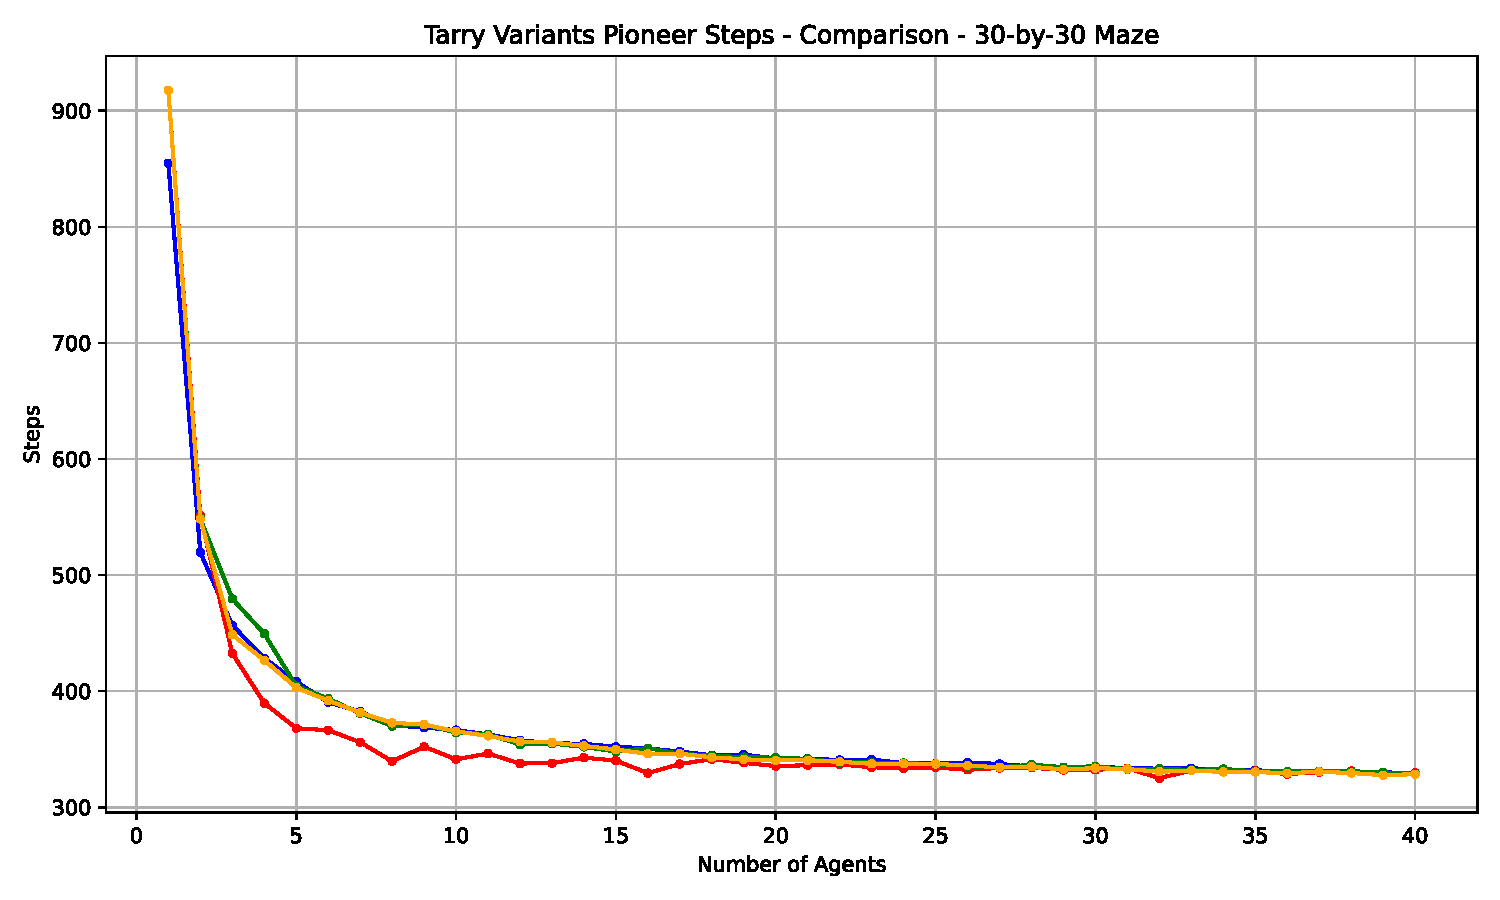
\includegraphics[width=0.45\linewidth]{Cap3/tarry_var_steps__30_by_30_maze.pdf} }}
    \qquad
    \subfloat[\centering 40x40 Maze]
    {{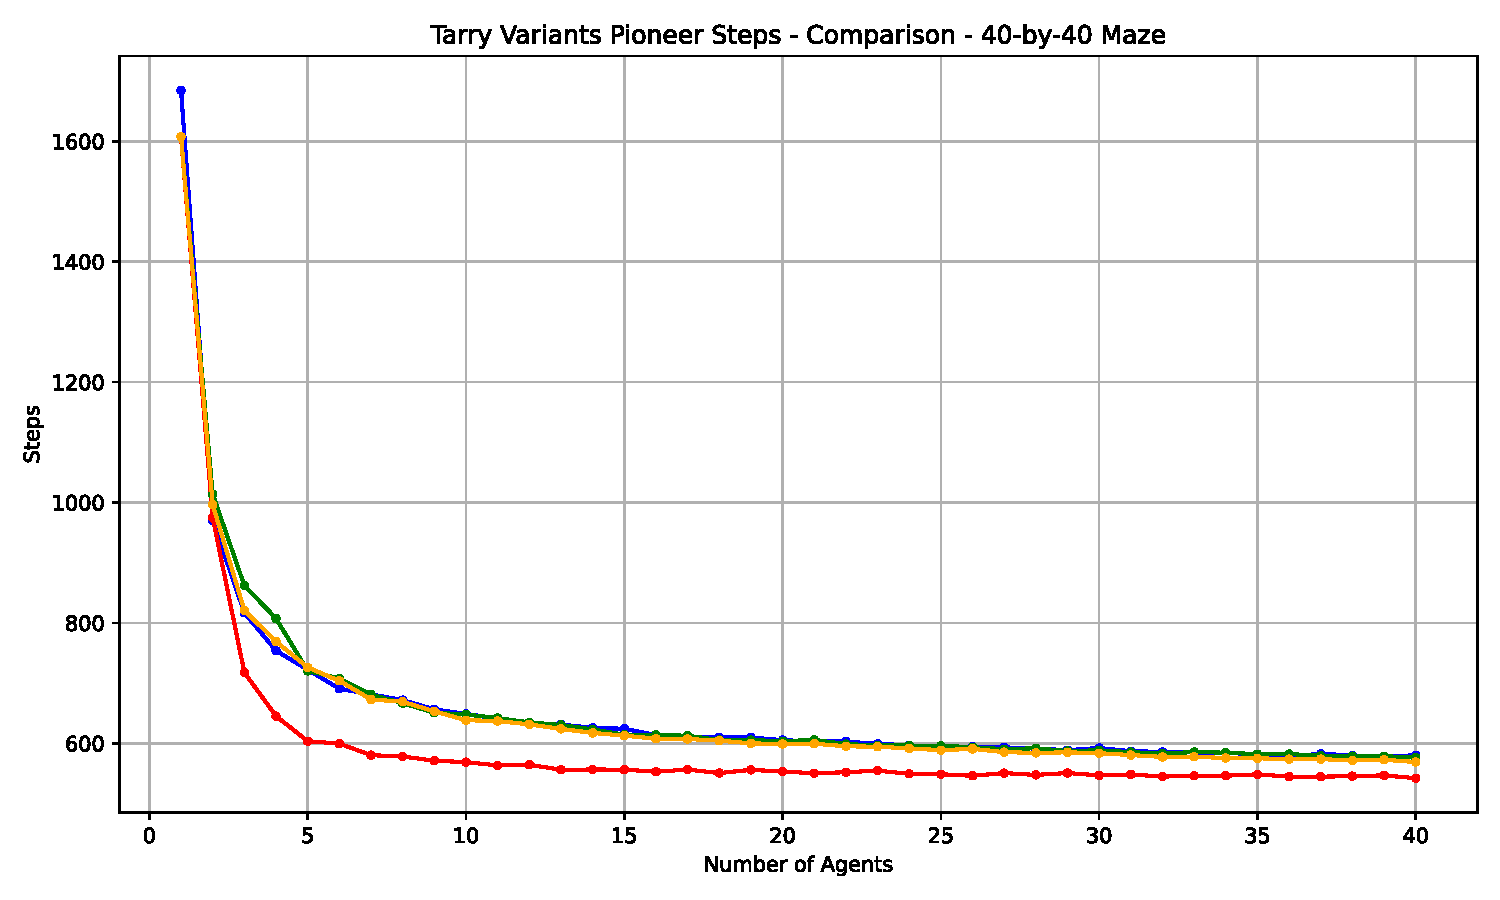
\includegraphics[width=0.45\linewidth]{Cap3/tarry_var_steps__40_by_40_maze.pdf} }}
    \caption{Comparison of the pioneer's average steps across Tarry's algorithm and its variations for different sizes of perfect mazes. The subfigures illustrate how algorithm performance changes with maze size.}
    \label{fig_tarry_steps_all_sizes_maze}
\end{figure}

\begin{figure}[H]
    \centering
    \qquad
    \qquad
    \subfloat[\centering Legend]
    {{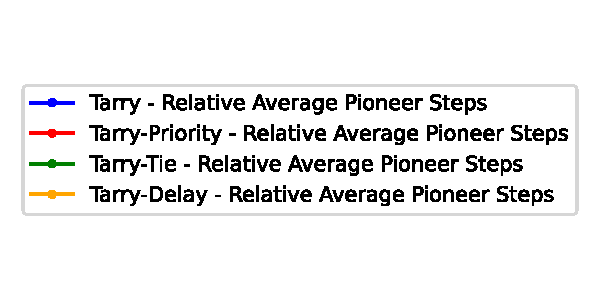
\includegraphics[width=0.5\textwidth]{Cap3/tarry_var_steps_legend_relative.pdf} }}
    \newline
    \subfloat[\centering 10x10 Maze]
    {{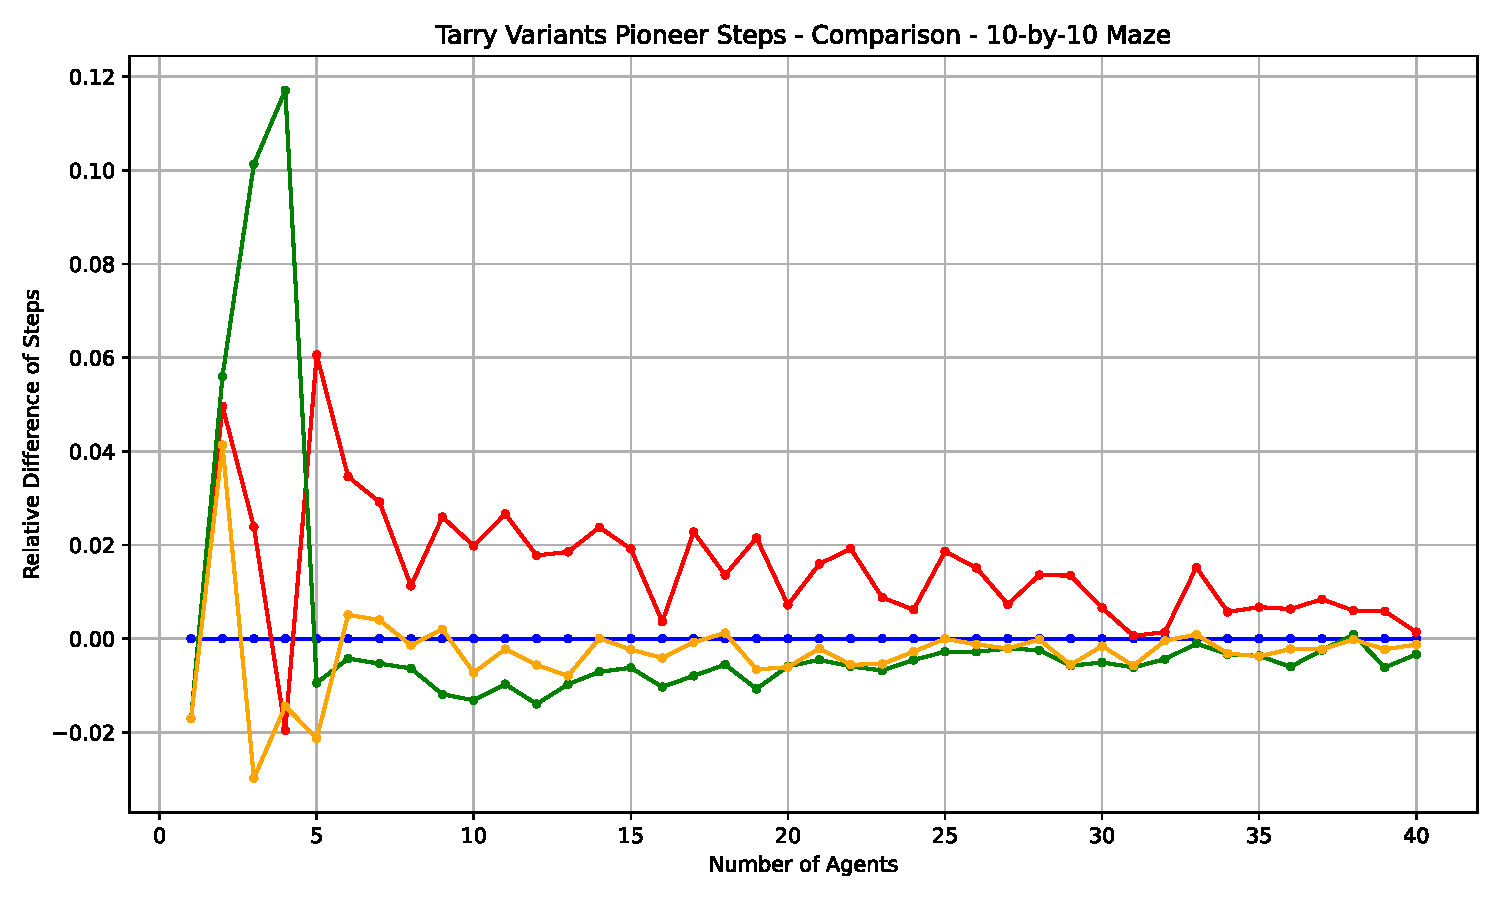
\includegraphics[width=0.45\linewidth]{Cap3/tarry_var_steps__10_by_10_maze_relative.pdf} }}
    \qquad
    \subfloat[\centering 20x20 Maze]
    {{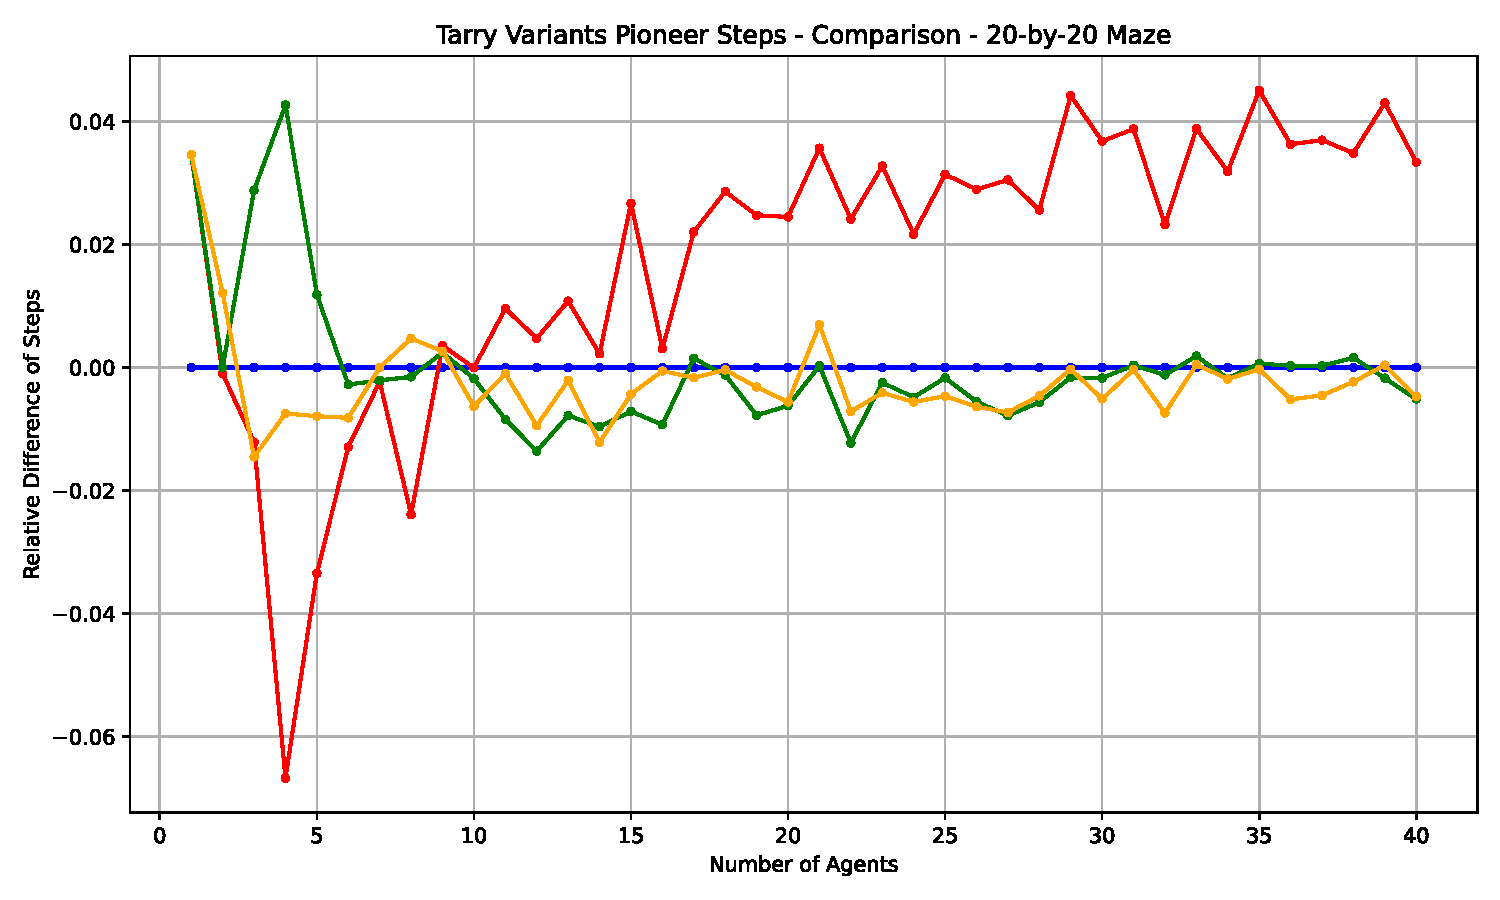
\includegraphics[width=0.45\linewidth]{Cap3/tarry_var_steps__20_by_20_maze_relative.pdf} }}
    \newline
    \subfloat[\centering 30x30 Maze]
    {{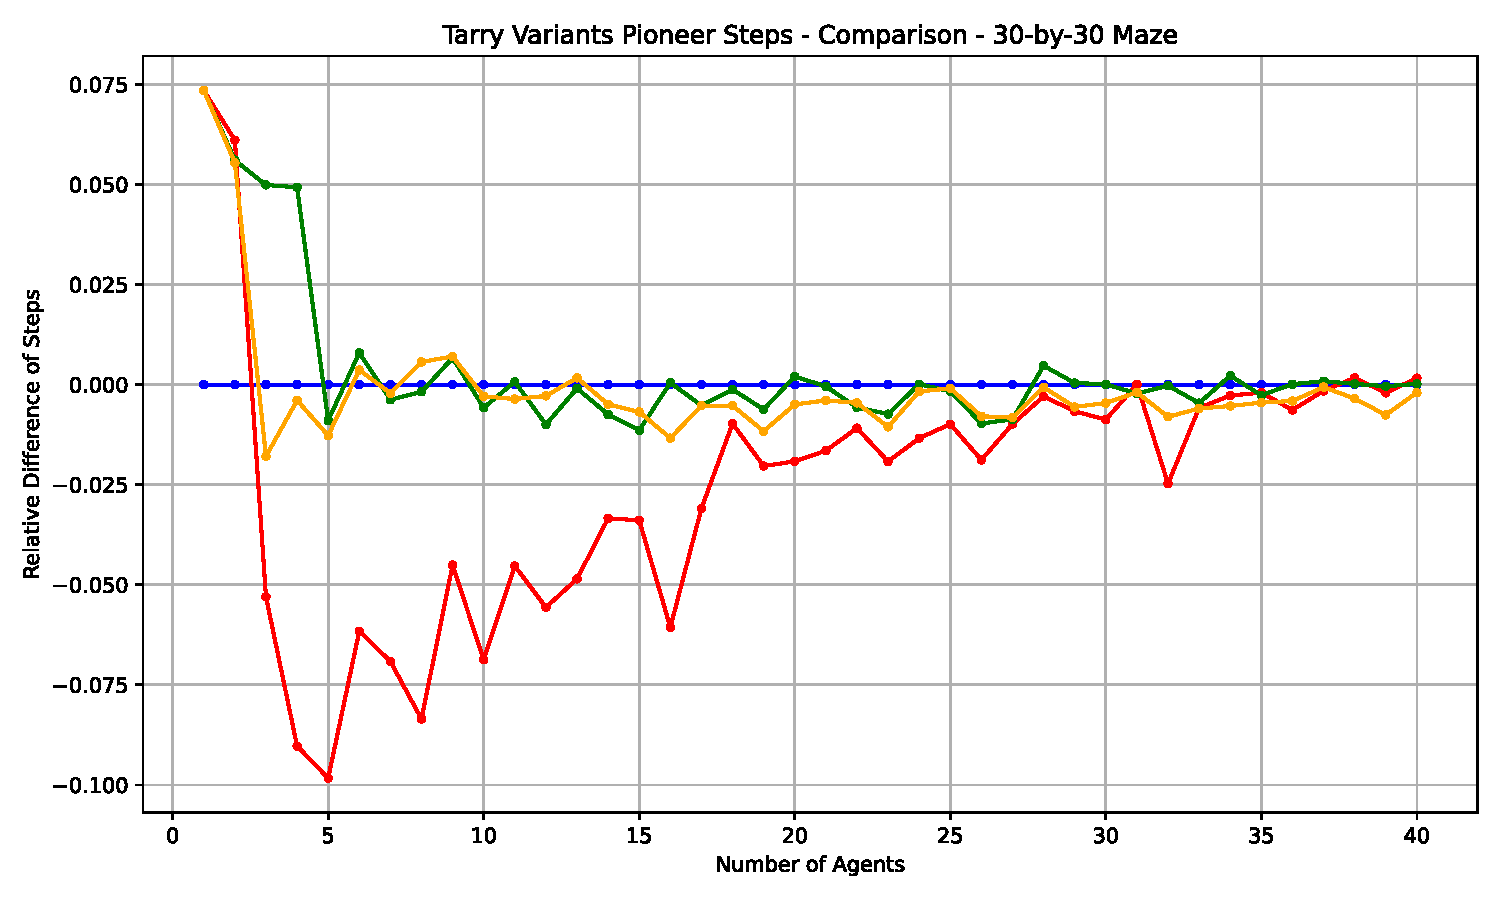
\includegraphics[width=0.45\linewidth]{Cap3/tarry_var_steps__30_by_30_maze_relative.pdf} }}
    \qquad
    \subfloat[\centering 40x40 Maze]
    {{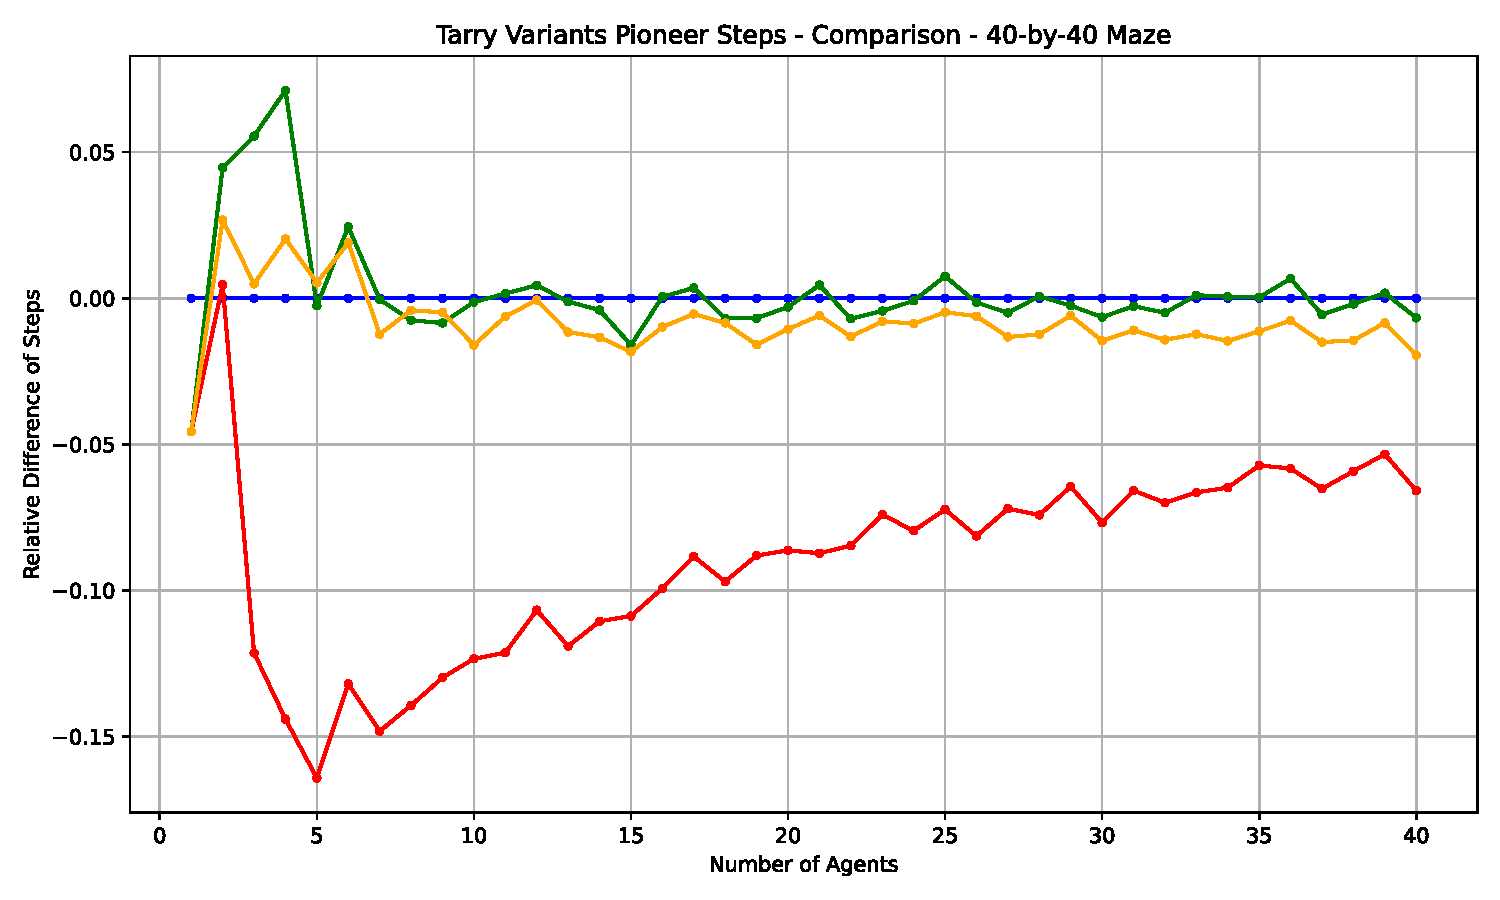
\includegraphics[width=0.45\linewidth]{Cap3/tarry_var_steps__40_by_40_maze_relative.pdf} }}
    \caption{Relative difference in pioneer steps between Tarry's algorithm variants and the original Tarry's algorithm, across different sizes of perfect mazes. The subfigures illustrate how the relative performance changes with maze size.}
    \label{fig_tarry_steps_relative_all_sizes_maze}
\end{figure}

\begin{figure}[H]
    \centering
    \qquad
    \qquad
    \subfloat[\centering Legend]
    {{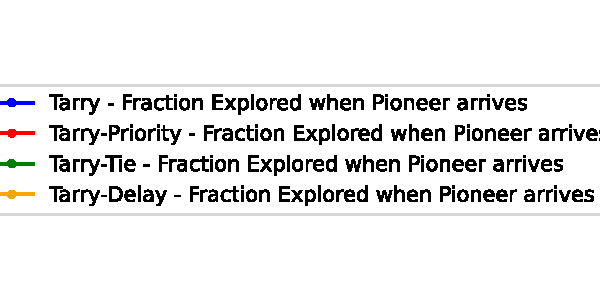
\includegraphics[width=0.5\textwidth]{Cap3/tarry_var_fraction_legend.pdf} }}
    \newline
    \subfloat[\centering 10x10 Maze]
    {{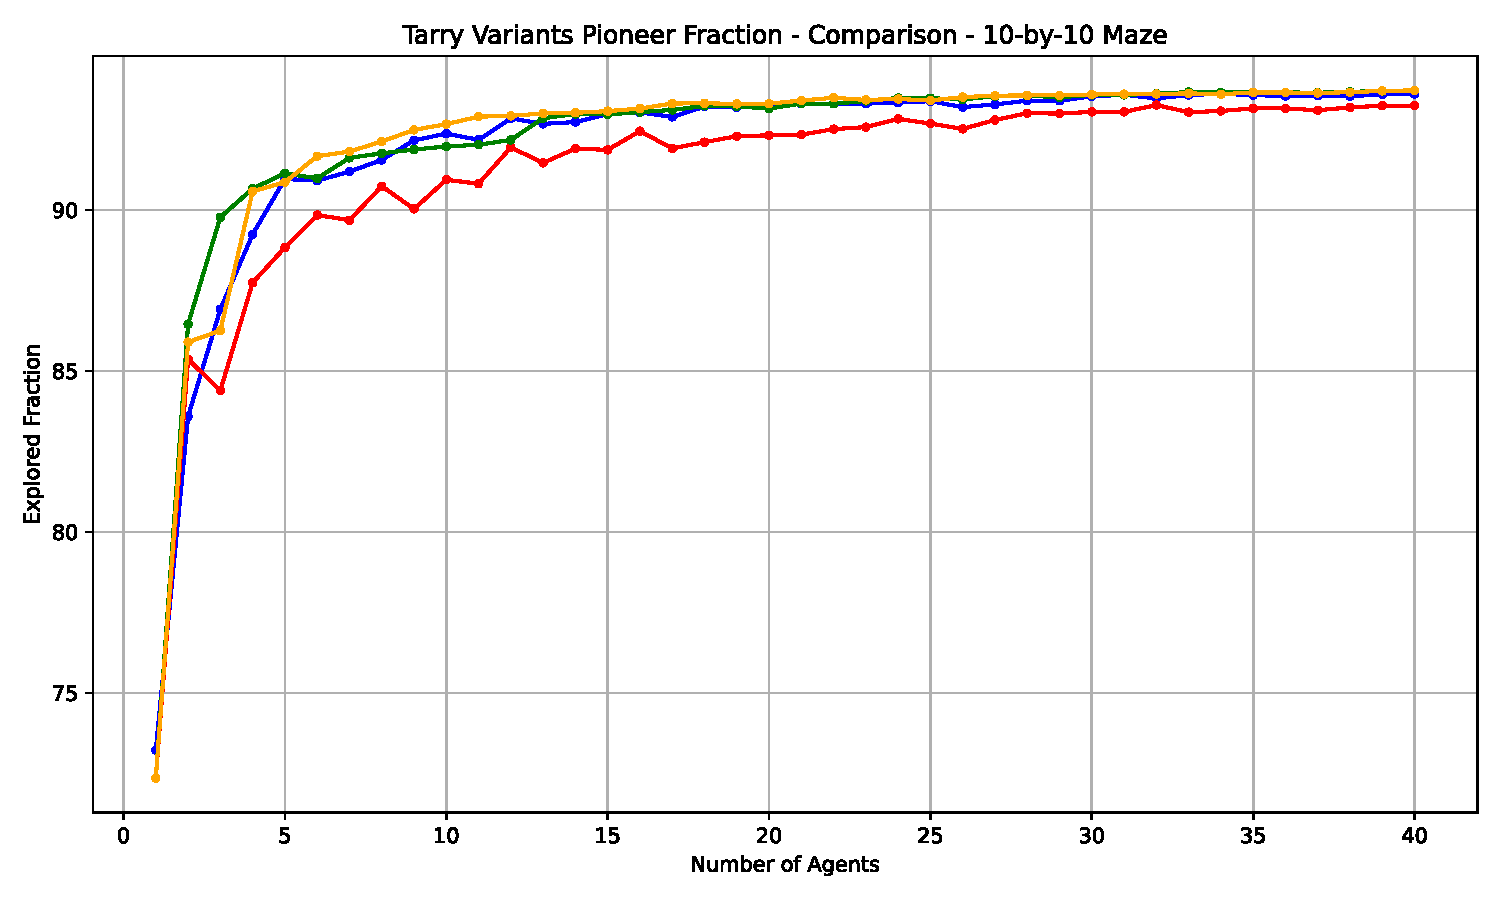
\includegraphics[width=0.45\linewidth]{Cap3/tarry_var_fraction__10_by_10_maze.pdf} }}
    \qquad
    \subfloat[\centering 20x20 Maze]
    {{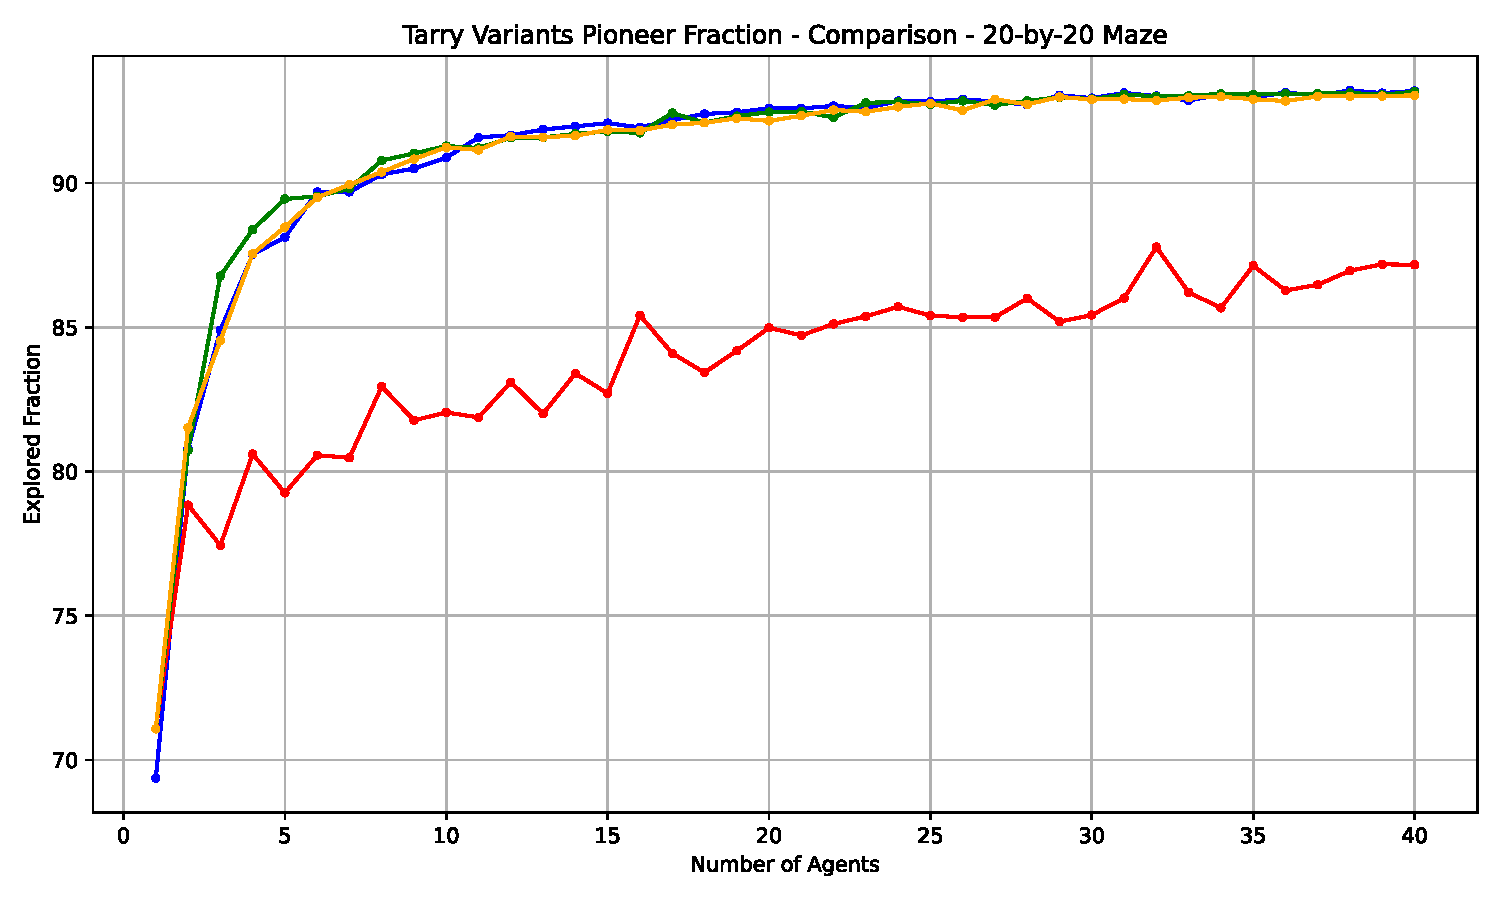
\includegraphics[width=0.45\linewidth]{Cap3/tarry_var_fraction__20_by_20_maze.pdf} }}
    \newline
    \subfloat[\centering 30x30 Maze]
    {{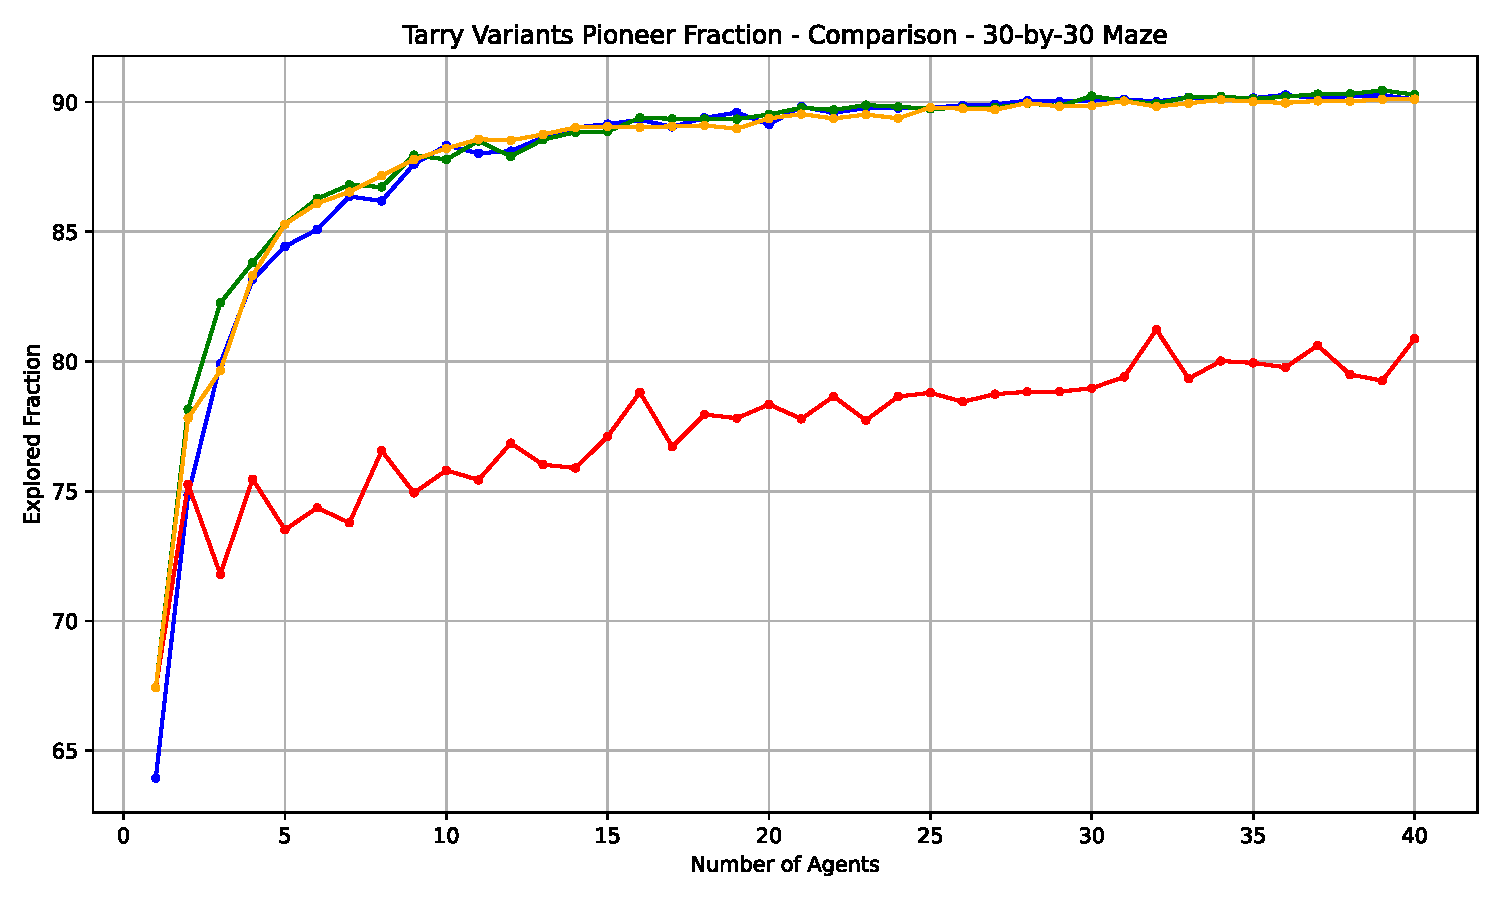
\includegraphics[width=0.45\linewidth]{Cap3/tarry_var_fraction__30_by_30_maze.pdf} }}
    \qquad
    \subfloat[\centering 40x40 Maze]
    {{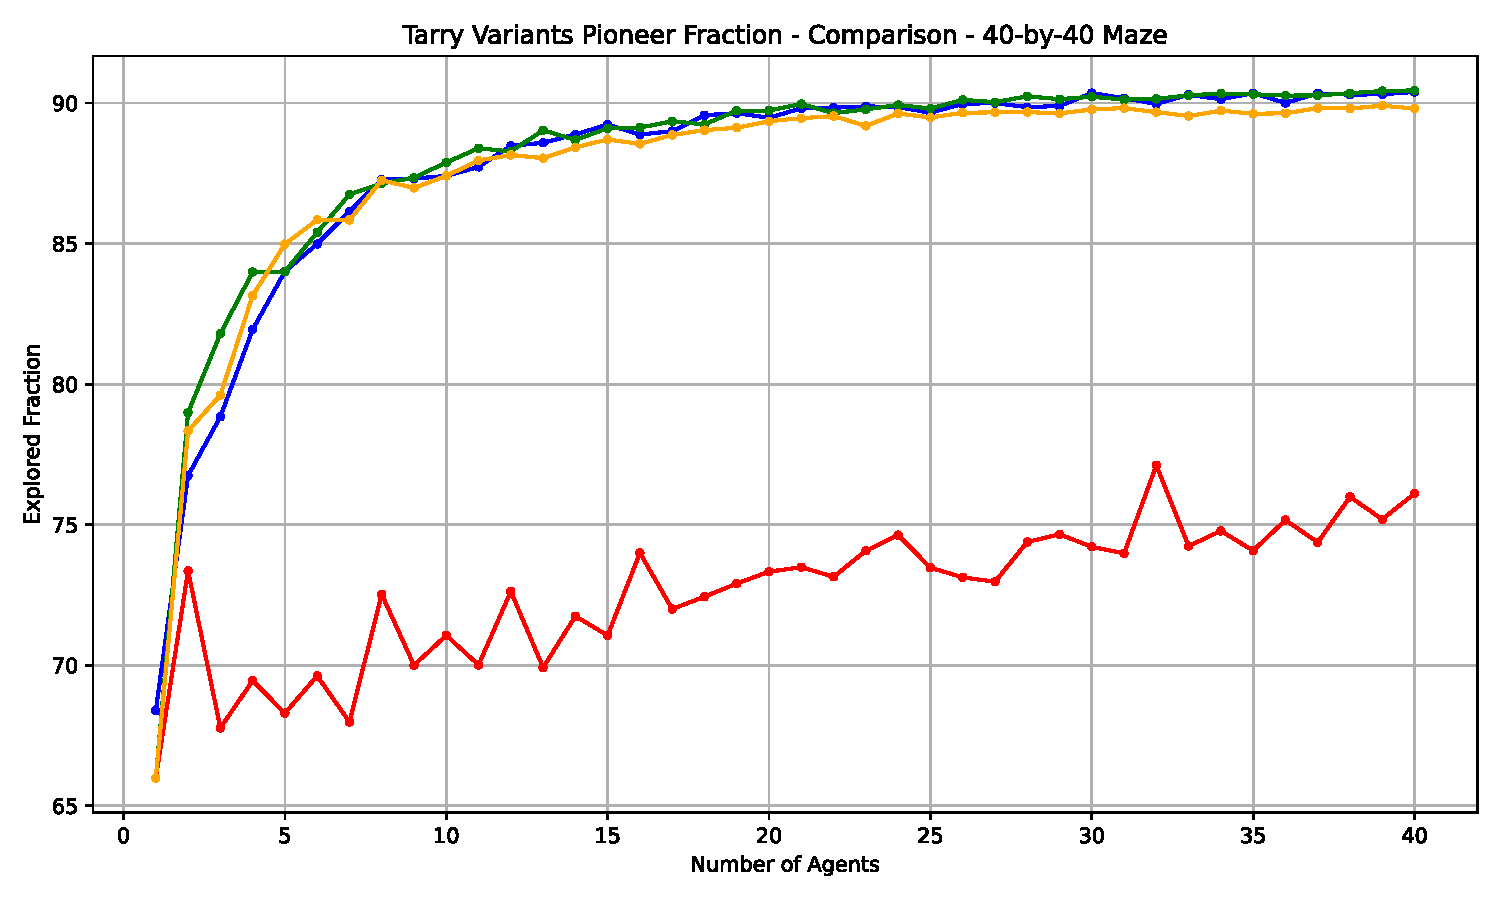
\includegraphics[width=0.45\linewidth]{Cap3/tarry_var_fraction__40_by_40_maze.pdf} }}
    \caption{Comparison of the explored fraction across Tarry's algorithm and its variations for different sizes of perfect mazes. The subfigures illustrate how the explored fraction changes with maze size.}
    \label{fig_tarry_fraction_all_sizes_maze}
\end{figure}
 
When analyzing Figures \ref{fig_tarry_steps_all_sizes_maze} and \ref{fig_tarry_steps_relative_all_sizes_maze}, it becomes evident that there is no uniform trend across all maze sizes. The Tarry Tie-Breaker and Delayed Tarry variations consistently outperform the standard Tarry algorithm, except in cases with a small number of agents. In those cases, early variations in exploration paths can significantly affect the outcome due to the extensive search required by each agent. However, a more intriguing behavior is observed with the Tarry Interval Priority variation. Although it performs similarly but slightly worse for smaller maze sizes, its performance improves for the largest maze analyzed. We conjecture this behavior can be attributed to the benefits of dispersion and the additional information obtained through interval filling, which only becomes significant during more extensive exploration. In mazes with considerable depth and narrow width, we believe interval filling initially causes conflicts, as agents may search for the start of their intervals in branches that have already been visited by others. However, in larger mazes, we assume these initial setbacks are offset by the advantages gained through the extra information during deeper exploration, which cannot be easily matched by Tarry's random choices.


An interesting observation can also be made regarding the explored fraction, as shown in Figure \ref{fig_tarry_fraction_all_sizes_maze}. The results indicate that the Tarry Interval Priority algorithm consistently explores a smaller portion of the graph compared to the other variations. Since mazes have few leaf nodes and communication prevents agents from overlapping in explored branches, the use of intervals likely directs agents more efficiently toward unexplored areas, potentially allowing them to head directly to leaf nodes before finding the actual solution.


\subsection{Random Tree Results} 
\label{subsection_tarry_random_tree_results}


The results for the random trees, using the same sizes as in Section \ref{subsection_no_comm_random_tree_results}, are presented in Figures \ref{fig_tarry_steps_all_sizes_tree}, \ref{fig_tarry_fraction_all_sizes_tree}, and \ref{fig_tarry_steps_relative_all_sizes_tree}.

\begin{figure}[H]
    \centering
    \qquad
    \qquad
    \subfloat[\centering Legend] 
    {{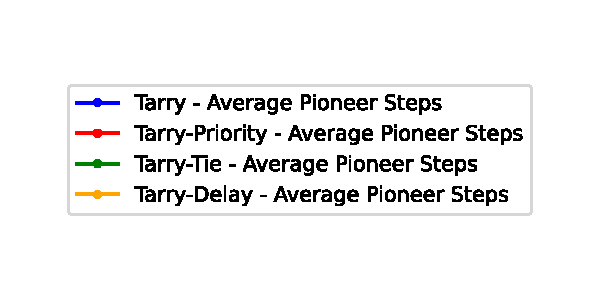
\includegraphics[width=0.5\textwidth]{Cap3/tarry_var_steps_legend.pdf} }}
    \newline
    \subfloat[\centering 100-node Tree]
    {{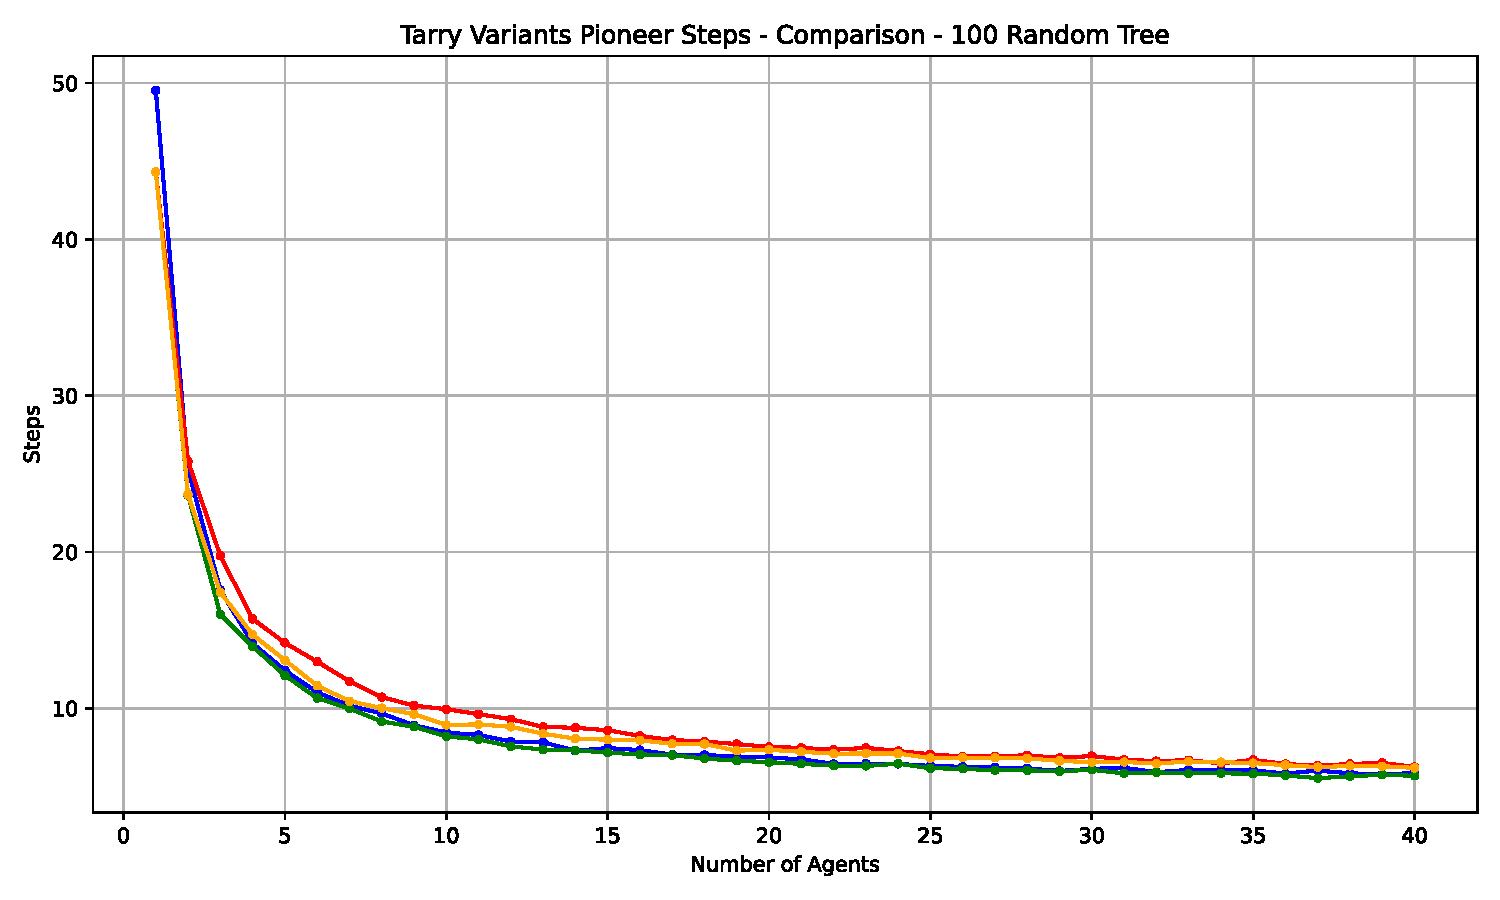
\includegraphics[width=0.45\linewidth]{Cap3/tarry_var_steps__100_tree.pdf} }}
    \qquad
    \subfloat[\centering 500-node Tree]
    {{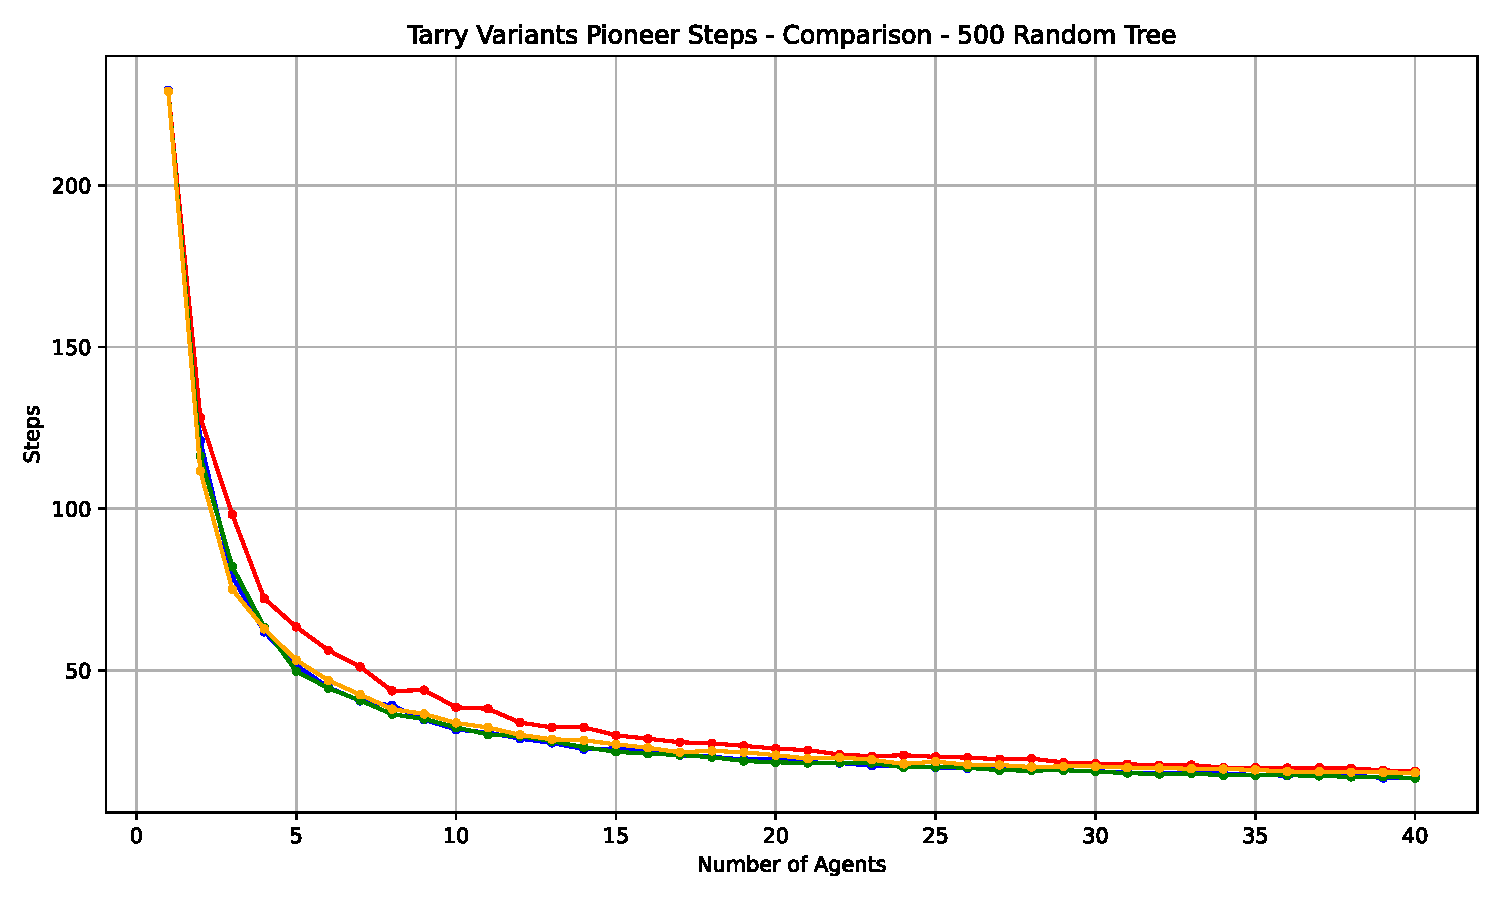
\includegraphics[width=0.45\linewidth]{Cap3/tarry_var_steps__500_tree.pdf} }}
    \newline
    \subfloat[\centering 1500-node Tree]
    {{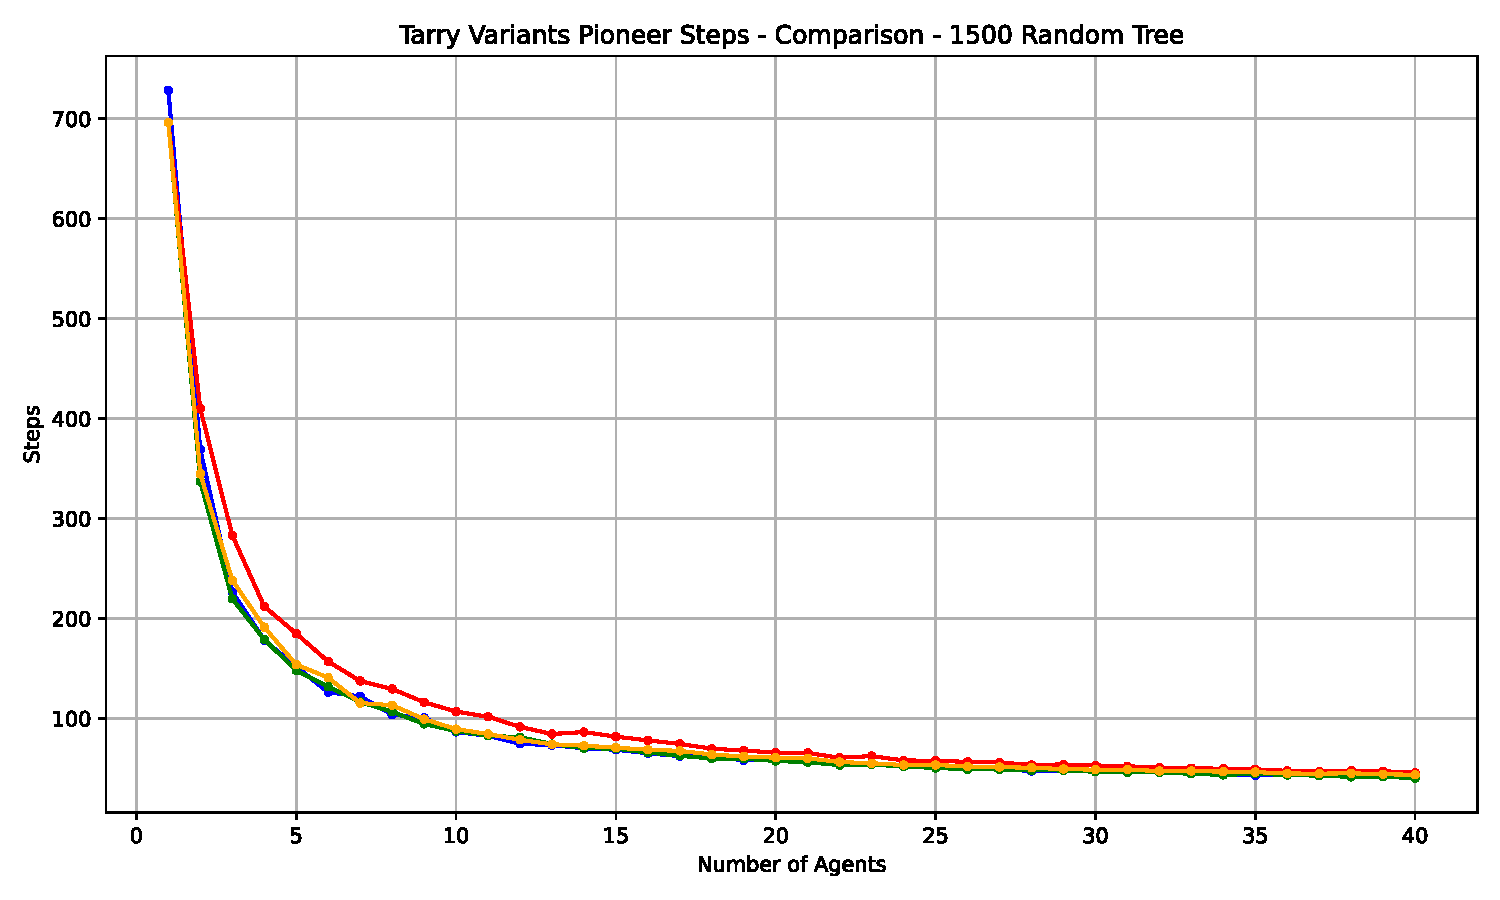
\includegraphics[width=0.45\linewidth]{Cap3/tarry_var_steps__1500_tree.pdf} }} 
    \caption{Comparison of the pioneer's average steps across Tarry's algorithm and its variations for different sizes of random trees. The subfigures illustrate how algorithm performance changes with tree size.} 
    \label{fig_tarry_steps_all_sizes_tree} 
\end{figure}

\begin{figure}[H]
    \centering
    \qquad
    \qquad
    \subfloat[\centering Legend]
    {{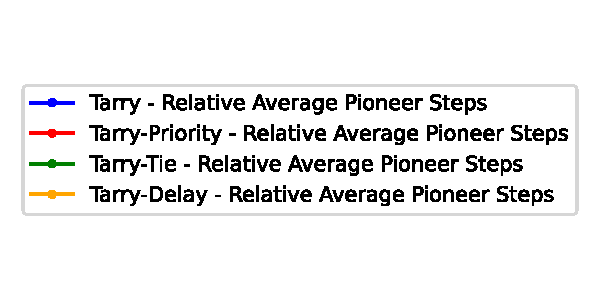
\includegraphics[width=0.5\textwidth]{Cap3/tarry_var_steps_legend_relative.pdf} }}
    \newline
    \subfloat[\centering 100-node Tree]
    {{\includegraphics[width=0.45\linewidth]{Cap3/tarry_var_steps__100_tree_relative.pdf} }}
    \qquad 
    \subfloat[\centering 500-node Tree]
    {{\includegraphics[width=0.45\linewidth]{Cap3/tarry_var_steps__500_tree_relative.pdf} }}
    \newline
    \subfloat[\centering 1500-node Tree]
    {{\includegraphics[width=0.45\linewidth]{Cap3/tarry_var_steps__1500_tree_relative.pdf} }} 
    \caption{Relative difference in pioneer steps between Tarry's algorithm variants and the original Tarry's algorithm across different sizes of random trees. The subfigures illustrate how the relative performance changes with tree size.} 
    \label{fig_tarry_steps_relative_all_sizes_tree}
\end{figure}

\begin{figure}[H]
    \centering
    \qquad
    \qquad
    \subfloat[\centering Legend]
    {{\includegraphics[width=0.5\textwidth]{Cap3/tarry_var_fraction_legend.pdf} }} 
    \newline 
    \subfloat[\centering 100-node Tree]
    {{\includegraphics[width=0.45\linewidth]{Cap3/tarry_var_fraction__100_tree.pdf} }}
    \qquad
    \subfloat[\centering 500-node Tree]
    {{\includegraphics[width=0.45\linewidth]{Cap3/tarry_var_fraction__500_tree.pdf} }}
    \newline 
    \subfloat[\centering 1500-node Tree]
    {{\includegraphics[width=0.45\linewidth]{Cap3/tarry_var_fraction__1500_tree.pdf} }}
    \caption{Comparison of the explored fraction across Tarry's algorithm and its variations for different sizes of random trees. The subfigures illustrate how the explored fraction changes with tree size.} 
    \label{fig_tarry_fraction_all_sizes_tree} 
\end{figure}

According to Figures \ref{fig_tarry_steps_all_sizes_tree} and \ref{fig_tarry_steps_relative_all_sizes_tree}, the results show a distinct pattern compared to those observed in Section \ref{subsection_tarry_maze_results}. The Tarry Interval Priority variation consistently underperforms across all tree sizes, with the disparity becoming even more pronounced when the number of agents is small. This outcome is likely due to the wide structure of the trees, where each agent in this variation needs to explore many leaf nodes within its assigned interval, resulting in inefficiencies. In contrast, only the Tarry Tie-Breaker shows small but consistent improvement for smaller number of nodes, although this advantage tends to disappear for larger trees.


When examining Figure \ref{fig_tarry_fraction_all_sizes_tree}, a similar behavior to what was previously discussed in Figure \ref{fig_no_comm_fraction_all_sizes_tree} can be observed. The explored fraction displays a pattern that is largely independent of the strategy used, due to the high variability in the fraction of nodes explored across different tree instances.

\subsection{Barabási-Albert Results} 
\label{subsection_tarry_barabasi_albert_results}

The results for the Barabási-Albert graphs, using the same sizes as in Section \ref{subsection_no_comm_barabasi_albert_results}, are presented in Figures \ref{fig_tarry_steps_all_sizes_barabasi}, \ref{fig_tarry_fraction_all_sizes_barabasi}, and \ref{fig_tarry_steps_relative_all_sizes_barabasi}.


\begin{figure}[H]
    \centering
    \qquad
    \qquad
    \subfloat[\centering Legend] 
    {{\includegraphics[width=0.5\textwidth]{Cap3/tarry_var_steps_legend.pdf} }}
    \newline
    \subfloat[\centering 100-node Barabási-Albert]
    {{\includegraphics[width=0.45\linewidth]{Cap3/tarry_var_steps__100_barabasi.pdf} }}
    \qquad
    \subfloat[\centering 250-node Barabási-Albert]
    {{\includegraphics[width=0.45\linewidth]{Cap3/tarry_var_steps__250_barabasi.pdf} }}
    \newline
    \subfloat[\centering 500-node Barabási-Albert]
    {{\includegraphics[width=0.45\linewidth]{Cap3/tarry_var_steps__500_barabasi.pdf} }}
    \qquad
    \subfloat[\centering 1000-node Barabási-Albert]
    {{\includegraphics[width=0.45\linewidth]{Cap3/tarry_var_steps__1000_barabasi.pdf} }} 
    \caption{Comparison of the pioneer's average steps across Tarry's algorithm and its variations for different sizes of Barabási-Albert graphs. The subfigures illustrate how algorithm performance changes with graph size.} 
    \label{fig_tarry_steps_all_sizes_barabasi} 
\end{figure}

\begin{figure}[H]
    \centering
    \qquad
    \qquad
    \subfloat[\centering Legend]
    {{\includegraphics[width=0.5\textwidth]{Cap3/tarry_var_steps_legend_relative.pdf} }}
    \newline
    \subfloat[\centering 100-node Barabási-Albert]
    {{\includegraphics[width=0.45\linewidth]{Cap3/tarry_var_steps__100_barabasi_relative.pdf} }}
    \qquad 
    \subfloat[\centering 250-node Barabási-Albert]
    {{\includegraphics[width=0.45\linewidth]{Cap3/tarry_var_steps__250_barabasi_relative.pdf} }}
    \newline
    \subfloat[\centering 500-node Barabási-Albert]
    {{\includegraphics[width=0.45\linewidth]{Cap3/tarry_var_steps__500_barabasi_relative.pdf} }}
    \qquad
    \subfloat[\centering 1000-node Barabási-Albert]
    {{\includegraphics[width=0.45\linewidth]{Cap3/tarry_var_steps__1000_barabasi_relative.pdf} }} 
    \caption{Relative difference in pioneer steps between Tarry's algorithm variants and the original Tarry's algorithm across different sizes of Barabási-Albert graphs. The subfigures illustrate how the relative performance changes with graph size.} 
    \label{fig_tarry_steps_relative_all_sizes_barabasi}
\end{figure}

\begin{figure}[H]
    \centering
    \qquad
    \qquad
    \subfloat[\centering Legend]
    {{\includegraphics[width=0.5\textwidth]{Cap3/tarry_var_fraction_legend.pdf} }} 
    \newline 
    \subfloat[\centering 100-node Barabási-Albert]
    {{\includegraphics[width=0.45\linewidth]{Cap3/tarry_var_fraction__100_barabasi.pdf} }}
    \qquad
    \subfloat[\centering 250-node Barabási-Albert]
    {{\includegraphics[width=0.45\linewidth]{Cap3/tarry_var_fraction__250_barabasi.pdf} }}
    \newline 
    \subfloat[\centering 500-node Barabási-Albert]
    {{\includegraphics[width=0.45\linewidth]{Cap3/tarry_var_fraction__500_barabasi.pdf} }}
    \qquad
    \subfloat[\centering 1000-node Barabási-Albert]
    {{\includegraphics[width=0.45\linewidth]{Cap3/tarry_var_fraction__1000_barabasi.pdf} }}
    \caption{Comparison of the explored fraction across Tarry's algorithm and its variations for different sizes of Barabási-Albert graphs. The subfigures illustrate how the explored fraction changes with graph size.} 
    \label{fig_tarry_fraction_all_sizes_barabasi} 
\end{figure}

Examining Figures \ref{fig_tarry_steps_all_sizes_barabasi} and \ref{fig_tarry_steps_relative_all_sizes_barabasi}, the poorer performance of the Tarry Interval Priority variation stands out. The results closely resemble those from the no-communication algorithms in \ref{subsection_no_comm_barabasi_albert_results}, likely due to the high connectivity in Barabási-Albert graphs. This structure accelerates exploration, often completing before an agent exhausts its interval, thus yielding similar outcomes.

Additionally, while the Tie-Breaker and Delayed Tarry variations perform worse than base Tarry on smaller datasets, they tend to improve, becoming consistently comparable or superior as graph size increases.

As expected, the explored fraction of the graph before the pioneer reaches the goal shows the same downward trend observed in \ref{subsection_no_comm_barabasi_albert_results}, with a smaller explored fraction as more agents are added. For larger Barabási-Albert graphs, the choice of algorithm has little impact on the explored fraction; however, for the smaller 100-node graph, Tarry's and the Tarry Tie-Breaker variation tend to explore less.
    
    

\chapter{Conclusions and Future Works}
This work presented an algorithm for graph exploration in a multi-agent system without communication, 
expanding on the solution proposed by \citen{Arthur2023}.
The flexibility provided by our framework,
which no longer relies on the open-source perfect maze generator by \citen{Naeem2021},
allows for expansion to various exploration policies and algorithmic variations.
Additionally, the modular design of our system enables integration of new exploration
strategies, paving the way for future advancements.

We conducted tests on 100 randomly generated 40x40 perfect mazes
and compared the results across three algorithms: 
our own, a backward interval variation, 
and an extended version of Tarry's algorithm. 
The results were validated against previous work \cite{Arthur2023},
confirming the correctness and reliability of our approach.

Looking forward, we aim to validate our algorithm
against established graph generation algorithms,
assessing its efficiency on a larger scale.
Exploring the implementation of more advanced algorithms
and optimizing the agents' decision-making processes will be essential
for enhancing the applicability of our approach.

By advancing multi-agent graph exploration without communication,
this research paves the way for innovations in autonomous systems,
with potential applications across various domains to be explored in future research.

% TODO:(RAFAEL): Change this Conclusion


% REFERENCIAS BIBLIOGRAFICAS
\renewcommand\bibname{\itareferencesnamebabel} %renomear título do capítulo referências
\bibliography{Referencias/referencias}

% Apendices
%\appendix
%\chapter{Tópicos de Dilema Linear} %opcional
%\section{Detailed Step-by-Step Execution}
\label{section_appendix_step_by_step}

This section provides a detailed step-by-step exploration of the graph shown in Figure \ref{fig_imperfect_maze_exploration}. The process is illustrated for all three agents, with each step specifying the intervals calculated for each child node. Nodes that would create cycles are marked in red, and the corresponding edges are represented as dotted lines. To maintain clarity and conciseness, some straightforward steps, such as those involving simple backtracking or non-decision points, are omitted. This ensures a focused understanding of how the agents navigate and construct their respective exploration trees.

The following figures present the step-by-step exploration process for each agent, highlighting their decisions and progress throughout the graph.

\begin{figure}[H]
    \centering
    \includegraphics[width=0.8\textwidth]{ApeA/maze_agent_1_step_0.png}
    \caption{Agent 1 - Starting Node for graph from Figure \ref{fig_imperfect_maze_exploration}.}
    \label{fig_agent_1_step_0}
\end{figure}

\begin{figure}[H]
    \centering
    \includegraphics[width=0.8\textwidth]{ApeA/maze_agent_2_step_0.png}
    \caption{Agent 2 - Starting Node for graph from Figure \ref{fig_imperfect_maze_exploration}.}
    \label{fig_agent_2_step_0}
\end{figure}

\begin{figure}[H]
    \centering
    \includegraphics[width=0.8\textwidth]{ApeA/maze_agent_3_step_0.png}
    \caption{Agent 3 - Starting Node for graph from Figure \ref{fig_imperfect_maze_exploration}.}
    \label{fig_agent_3_step_0}
\end{figure}

\begin{figure}[H]
    \centering
    \includegraphics[width=0.8\textwidth]{ApeA/maze_agent_1_step_1.png}
    \caption{Agent 1 - First Step exploring the graph.}
    \label{fig_agent_1_step_1}
\end{figure}

\begin{figure}[H]
    \centering
    \includegraphics[width=0.8\textwidth]{ApeA/maze_agent_2_step_1.png}
    \caption{Agent 2 - First Step exploring the graph.}
    \label{fig_agent_2_step_1}
\end{figure}

\begin{figure}[H]
    \centering
    \includegraphics[width=0.8\textwidth]{ApeA/maze_agent_3_step_1.png}
    \caption{Agent 3 - First Step exploring the graph.}
    \label{fig_agent_3_step_1}
\end{figure}

\begin{figure}[H]
    \centering
    \includegraphics[width=0.8\textwidth]{ApeA/maze_agent_1_step_2.png}
    \caption{Agent 1 - Second Step exploring the graph.}
    \label{fig_agent_1_step_2}
\end{figure}

\begin{figure}[H]
    \centering
    \includegraphics[width=0.8\textwidth]{ApeA/maze_agent_2_step_2.png}
    \caption{Agent 2 - Second Step exploring the graph.}
    \label{fig_agent_2_step_2}
\end{figure}

\begin{figure}[H]
    \centering
    \includegraphics[width=0.8\textwidth]{ApeA/maze_agent_3_step_2.png}
    \caption{Agent 3 - Second Step exploring the graph.}
    \label{fig_agent_3_step_2}
\end{figure}

\begin{figure}[H]
    \centering
    \includegraphics[width=0.8\textwidth]{ApeA/maze_agent_1_step_3.png}
    \caption{Agent 1 - Multiple Steps of exploration.}
    \label{fig_agent_1_step_3}
\end{figure}

\begin{figure}[H]
    \centering
    \includegraphics[width=0.8\textwidth]{ApeA/maze_agent_2_step_3.png}
    \caption{Agent 2 - Multiple Steps of exploration.}
    \label{fig_agent_2_step_3}
\end{figure}

\begin{figure}[H]
    \centering
    \includegraphics[width=0.8\textwidth]{ApeA/maze_agent_3_step_3.png}
    \caption{Agent 3 - Multiple Steps of exploration.}
    \label{fig_agent_3_step_3}
\end{figure}

\begin{figure}[H]
    \centering
    \includegraphics[width=1\textwidth]{ApeA/maze_agent_1_step_4.png}
    \caption{Agent 1 - Final exploration steps.}
    \label{fig_agent_1_step_4}
\end{figure}

\begin{figure}[H]
    \centering
    \includegraphics[width=1\textwidth]{ApeA/maze_agent_2_step_4.png}
    \caption{Agent 2 - Final exploration steps.}
    \label{fig_agent_2_step_4}
\end{figure}

\begin{figure}[H]
    \centering
    \includegraphics[width=1\textwidth]{ApeA/maze_agent_3_step_4.png}
    \caption{Agent 3 - Final exploration steps.}
    \label{fig_agent_3_step_4}
\end{figure}



% Anexos
%\annex
%\chapter{Exemplo de um Primeiro Anexo} %opcional
%\input{AneA/anexoA}

% Glossario
%\itaglossary
%\printglossary

% Folha de Registro do Documento
% Valores dos campos do formulario
\FRDitadata{X de Novembro de 2024}
\FRDitadocnro{DCTA/ITA/?/2024} %(o número de registro você solicita a biblioteca)
\FRDitaorgaointerno{Instituto Tecnológico de Aeronáutica -- ITA}
%Exemplo no caso de pós-graduação: Instituto Tecnol{\'o}gico de Aeron{\'a}utica -- ITA
\FRDitapalavrasautor{Graph, Search, Multi-Agent, Mixed-Radix}
\FRDitapalavrasresult{?}
%Exemplo no caso de graduação (TG):
\FRDitapalavraapresentacao{ITA, São José dos Campos. Curso de Graduação em Engenharia de Computação. Orientador: Prof. Dr. Luiz Gustavo Bizarro Mirisola; coorientador: Prof. Dr. Vitor Venceslau Curtis. Publicado em 2024.}
%Exemplo no caso de pós-graduação (msc, dsc):
%\FRDitapalavraapresentacao{ITA, São José dos Campos. Curso de Mestrado. Programa de Pós-Graduação em Engenharia Aeronáutica e Mecânica. Área de Sistemas Aeroespaciais e Mecatrônica. Orientador: Prof.~Dr. Adalberto Santos Dupont. Coorientadora: Prof$^\textnormal{a}$.~Dr$^\textnormal{a}$. Doralice Serra. Defesa em 05/03/2015. Publicada em 16/06/2023.}
\FRDitaresumo{Graph theory, a pivotal field in mathematics and computer science, offers robust frameworks for modeling relationships and traversing graph structures. This research delves into graph exploration, crucial for applications like network routing, robotics, and procedural generation. As real-world applications often involve complex environments with time constraints, such as search-and-rescue operations with drones, this study focuses on multi-agent systems for graph exploration, where multiple autonomous agents collaborate to optimize task distribution.

This work presents a modular framework structured into extensible classes, facilitating the addition of new algorithms and datasets. By moving beyond the constraints of perfect maze exploration \cite{Naeem2021}, we employed NetworkX \cite{Hagberg2008}—a general graph library—which allows for analyzing more diverse graph structures. This flexibility enabled comparisons across various datasets to reveal patterns in algorithm performance under different graph characteristics.

This study's objective is to propose an efficient multi-agent algorithm for graph exploration without communication, a crucial need in scenarios where communication is impractical or impossible. Building on the method for perfect maze exploration detailed by \citen{Arthur2023}, this study extends the approach to general graphs, including those with cycles, and evaluates the algorithm's performance across three datasets of varying complexity. By establishing a benchmark for exploration efficiency, this research enables an assessment of the costs and benefits of incorporating communication in multi-agent strategies, providing a comparative baseline for future exploration algorithm development.

Additionally, this research incorporated heuristics and alternative strategies to enhance Tarry's algorithm, which traditionally relies on random neighbor selection. The resulting adaptations demonstrated performance improvements on specific datasets, illustrating how targeted selection processes can optimize exploration efficiency based on dataset properties. These insights pave the way for future research into more effective graph exploration strategies in autonomous systems.}
%  Primeiro Parametro: Nacional ou Internacional -- N/I
%  Segundo parametro: Ostensivo, Reservado, Confidencial ou Secreto -- O/R/C/S
\FRDitaOpcoes{N}{O}
% Cria o formulario
\itaFRD

\end{document}
